\chapter{HASIL DAN PEMBAHASAN}

\section{Skenario Pengujian}
Penelitian ini menguji performa algoritma \textit{Artificial Bee Colony} (ABC) yang dikombinasikan dengan \textit{Elite Opposition-Based Learning} (EOBL) dalam berbagai skenario uji coba yang dirancang secara sistematis. Uji coba dilakukan menggunakan tiga jenis \textit{dataset} utama, yaitu \textit{Simple Random}, \textit{Stratified Random}, dan SDSC (\textit{San Diego Supercomputer Center}) \textit{Blue Horizon Log}. Setiap \textit{dataset} memiliki karakteristik dan ukuran yang berbeda, sehingga memberikan gambaran lengkap terhadap kemampuan algoritma dalam menghadapi berbagai kondisi penjadwalan tugas di lingkungan \textit{cloud computing}. Selain itu penelitian ini menguji performa pada \textit{real environment} agar mengetahui kondisi di lingkungan nyata.

\begin{table} [H]
    \centering
    \caption{Skenario algoritma, \textit{dataset} yang digunakan, dan iterasi pengujian}
    \begin{tblr}{
        hlines,
        vlines,
        colspec = {Q[c,m] Q[c,m] Q[c,m] Q[c,m] Q[r,m]},
        row{1} = {bg=blue!30, font=\bfseries},
    }
    No & Skenario  & Algoritma        & \textit{Dataset}          & Iterasi Pengujian \\
    1  & Skenario 1 & \SetCell[r=4]{m} ABC              & \textit{Simple Random}    & \SetCell[r=2]{m} 100 \\
    2  & Skenario 2 &                   & \textit{Stratified Random} &                    \\
    \cline{1-2, 4-4}
    3  & Skenario 3 &                   & SDSC             & \SetCell[r=2]{m} 10                 \\
    4  & Skenario 4 &                   & \textit{Real Environment}  &                    \\
    \cline{1-2, 4-4}
    5  & Skenario 5 & \SetCell[r=4]{m} ABC - EOBL      & \textit{Simple Random}    & \SetCell[r=2]{m} 100 \\
    6  & Skenario 6 &                   & \textit{Stratified Random} &                    \\
    \cline{1-2, 4-4}
    7  & Skenario 7 &                   & SDSC             & \SetCell[r=2]{m} 10                 \\
    8  & Skenario 8 &                   & \textit{Real Environment}  &                    \\
    \cline{1-2, 4-4}
    9  & Skenario 9 & \SetCell[r=4]{m} PSO              & \textit{Simple Random}    & \SetCell[r=2]{m} 100 \\
    10 & Skenario 10 &                  & \textit{Stratified Random} &                    \\
    \cline{1-2, 4-4}
    11 & Skenario 11 &                  & SDSC             & \SetCell[r=2]{m} 10                 \\
    12 & Skenario 12 &                  & \textit{Real Environment}  &                    \\
    \cline{1-2, 4-4}
    13 & Skenario 13 & \SetCell[r=4]{m} GA               & \textit{Simple Random}    & \SetCell[r=2]{m} 100 \\
    14 & Skenario 14 &                  & \textit{Stratified Random} &                    \\
    \cline{1-2, 4-4}
    15 & Skenario 15 &                  & SDSC             & \SetCell[r=2]{m} 10                 \\
    16 & Skenario 16 &                  & \textit{Real Environment}  &                    \\
    \end{tblr}
\end{table}

Pengujian pada \textit{dataset simple random} dan \textit{stratified random} dilakukan sebanyak 10 kali dengan 10 iterasi untuk setiap \textit{subset dataset}, yang masing-masing memiliki variasi ukuran mulai dari 1.000 hingga 10.000 tugas. Untuk \textit{dataset} SDSC, pengujian dilakukan dengan 10 iterasi mengingat karakteristik data historis yang lebih kompleks. Uji pada \textit{real environment} dilakukan sebanyak 10 iterasi untuk setiap algoritma. Dengan demikian, keseluruhan eksperimen mencakup total 220 kali pengujian untuk setiap algoritma, dan jika diuji dengan tiga algoritma berbeda, maka total pengujian mencapai 880 kali. Setiap algoritma juga diatur dengan parameter yang relevan untuk meningkatkan performa.

Hasil pengujian akan diukur menggunakan beberapa parameter kinerja yang telah ditetapkan, seperti \textit{makespan}, \textit{average start time}, \textit{average finish time}, \textit{resource utilization}, \textit{energy consumption}, dan \textit{imbalance degree}. Parameter-parameter ini disusun dalam tabel khusus untuk memudahkan analisis dan perbandingan kinerja algoritma secara menyeluruh

Dalam \textit{real environment}, terdapat pengecualian terhadap beberapa parameter yang digunakan karena tidak dapat diuji, seperti konsumsi energi. Hal ini disebabkan oleh keterbatasan data yang tersedia dari skema tersebut, sehingga kita tidak dapat mengetahui hasil dari beberapa parameter tersebut.

\subsubsection{Uji Coba Parameter dan Koefisien}
Sebelum melaksanakan pengujian utama, dilakukan uji coba awal untuk menentukan nilai-nilai parameter penting yang berpengaruh signifikan terhadap kinerja algoritma penjadwalan tugas di lingkungan \textit{cloud}. Parameter yang diuji meliputi ukuran populasi (\textit{population size}), jumlah iterasi maksimal (\textit{max iterations}), batas stagnasi solusi (\textit{limit}), serta koefisien pada metode \textit{Elite Opposition-Based Learning} (EOBL). Uji coba ini bertujuan untuk menemukan konfigurasi parameter yang memberikan keseimbangan optimal antara eksplorasi dan eksploitasi ruang solusi, sehingga dapat menghasilkan \textit{makespan} yang rendah, \textit{throughput} yang tinggi, dan pemanfaatan sumber daya yang optimal. Pengujian parameter ini menggunakan SDSC dikarenakan mengimplementasikan kasus yang nyata.

\subsubsection{A. \textit{Population Size}}

\begin{table} [H]
\centering
\caption{Rata-rata hasil percobaan untuk variasi ukuran populasi}
\begin{tabular}{|>{\raggedright\arraybackslash}m{0.15\linewidth}|
                >{\raggedleft\arraybackslash}m{0.17\linewidth}|
                >{\raggedleft\arraybackslash}m{0.17\linewidth}|
                >{\raggedleft\arraybackslash}m{0.17\linewidth}|
                >{\raggedleft\arraybackslash}m{0.17\linewidth}|}
\rowcolor{blue!30}
\hline
\multicolumn{1}{|>{\centering\arraybackslash}m{0.15\linewidth}|}{\textbf{Parameter}} & 
\multicolumn{1}{>{\centering\arraybackslash}m{0.17\linewidth}|}{\textbf{\textit{Population Size} = 30}} & 
\multicolumn{1}{>{\centering\arraybackslash}m{0.17\linewidth}|}{\textbf{\textit{Population Size} = 40}} & 
\multicolumn{1}{>{\centering\arraybackslash}m{0.17\linewidth}|}{\textbf{\textit{Population Size} = 50}} & 
\multicolumn{1}{>{\centering\arraybackslash}m{0.17\linewidth}|}{\textbf{\textit{Population Size} = 80}} \\
\hline
\textit{Average Waiting Time} (ms)      & 14,53      & 14,23      & 14,98      & 15,91      \\ \hline
\textit{Average Start Time} (ms)        & 27.231,43  & 28.461,11  & 28.724,93  & 30.312,11  \\ \hline
\textit{Average Execution Time} (ms)    & 354,14     & 350,71     & 350,42     & 345,30     \\ \hline
\textit{Average Finish Time} (ms)       & 27.585,57  & 28.811,82  & 29.075,35  & 30.657,42  \\ \hline
\textit{Throughput} (\textit{task}/s)                     & 0,0695     & 0,0706     & 0,0675     & 0,0631     \\ \hline
\textit{Makespan} (ms)                  & 107.475,00 & 105.291,60 & 110.865,30 & 117.641,40 \\ \hline
\textit{Imbalance Degree} (\%)          & 56,32      & 54,24      & 53,06      & 54,82      \\ \hline
\textit{Scheduling Length} (ms)   & 203.855.183,70 & 210.570.758,70 & 212.527.320,90 & 224.271.288,60 \\ \hline
\textit{Resource Utilization} (\%)      & 45,58      & 45,84      & 43,83      & 40,36      \\ \hline
\textit{Total Energy Consumption} (kWh) & 473,18     & 485,14     & 498,62     & 531,16     \\ \hline
\end{tabular}
\end{table}

Hasil pengujian menunjukkan bahwa ukuran populasi yang lebih kecil, sekitar 30 individu, mampu memberikan hasil \textit{makespan} yang rendah serta efisiensi pemanfaatan sumber daya yang lebih baik. Namun demikian, pada ukuran populasi kecil ini nilai \textit{imbalance degree} cenderung lebih tinggi dan kurang baik dibandingkan populasi yang lebih besar. Sebaliknya, penggunaan ukuran populasi yang terlalu besar justru cenderung memperlambat waktu konvergensi tanpa memberikan peningkatan signifikan terhadap kualitas solusi secara umum.

\newpage

\subsubsection{B. \textit{Limit}}

\begin{table} [H]
\centering
\caption{Rata-rata hasil percobaan untuk variasi \textit{limit}}
\begin{tabular}{|>{\raggedright\arraybackslash}m{0.15\linewidth}|
                >{\raggedleft\arraybackslash}m{0.17\linewidth}|
                >{\raggedleft\arraybackslash}m{0.17\linewidth}|
                >{\raggedleft\arraybackslash}m{0.17\linewidth}|
                >{\raggedleft\arraybackslash}m{0.17\linewidth}|}
\rowcolor{blue!30}
\hline
\multicolumn{1}{|>{\centering\arraybackslash}m{0.15\linewidth}|}{\textbf{Parameter}} & 
\multicolumn{1}{>{\centering\arraybackslash}m{0.17\linewidth}|}{\textbf{\textit{Limit} = 0,3}} & 
\multicolumn{1}{>{\centering\arraybackslash}m{0.17\linewidth}|}{\textbf{\textit{Limit} = 0,4}} & 
\multicolumn{1}{>{\centering\arraybackslash}m{0.17\linewidth}|}{\textbf{\textit{Limit} = 0,5}} & 
\multicolumn{1}{>{\centering\arraybackslash}m{0.17\linewidth}|}{\textbf{\textit{Limit} = 0,6}} \\
\hline
\textit{Average Waiting Time} (ms)      & 15,15      & 14,58      & 14,68      & 14,08      \\ \hline
\textit{Average Start Time} (ms)        & 27.261,75  & 27.872,08  & 27.275,30  & 27.569,17  \\ \hline
\textit{Average Execution Time} (ms)    & 353,11     & 352,45     & 352,69     & 352,89     \\ \hline
\textit{Average Finish Time} (ms)       & 27.614,86  & 28.224,52  & 27.627,99  & 27.922,06  \\ \hline
\textit{Throughput} (\textit{task}/s)                   & 0,0664     & 0,0697     & 0,0688     & 0,0706     \\ \hline
\textit{Makespan} (ms)                 & 112.081,20 & 108.159,90 & 108.618,90 & 105.296,10 \\ \hline
\textit{Imbalance Degree} (\%)         & 57,68      & 56,01      & 55,71      & 57,85      \\ \hline
\textit{Scheduling Length} (ms)  & 201.708.255,30 & 206.217.732,30 & 201.804.989,10 & 203.974.881,90 \\ \hline
\textit{Resource Utilization} (\%)     & 43,45      & 45,53      & 44,94      & 46,13      \\ \hline
\textit{Total Energy Consumption} (kWh) & 475,52    & 484,45     & 483,35     & 476,86     \\ \hline
\end{tabular}
\end{table}

Berdasarkan hasil eksperimen, nilai parameter \textit{limit} sebesar 0.6 menunjukkan hasil yang paling optimal ketika dikombinasikan dengan iterasi antara 10 hingga 15 dan ukuran populasi yang relatif kecil (30 individu). Kombinasi ini secara efektif menghasilkan \textit{makespan} yang lebih rendah, meningkatkan \textit{throughput}, serta memberikan utilisasi sumber daya yang lebih baik. 

\newpage

\subsubsection{C. \textit{Iteration}}

\begin{table} [H]
\centering
\caption{Rata-rata hasil percobaan untuk variasi iterasi maksimal}
\begin{tabular}{|>{\raggedright\arraybackslash}m{0.15\linewidth}|
                >{\raggedleft\arraybackslash}m{0.17\linewidth}|
                >{\raggedleft\arraybackslash}m{0.17\linewidth}|
                >{\raggedleft\arraybackslash}m{0.17\linewidth}|
                >{\raggedleft\arraybackslash}m{0.17\linewidth}|}
\rowcolor{blue!30}
\hline
\multicolumn{1}{|>{\centering\arraybackslash}m{0.15\linewidth}|}{\textbf{Parameter}} & 
\multicolumn{1}{>{\centering\arraybackslash}m{0.17\linewidth}|}{\textbf{\textit{Iteration} = 5}} & 
\multicolumn{1}{>{\centering\arraybackslash}m{0.17\linewidth}|}{\textbf{\textit{Iteration} = 10}} & 
\multicolumn{1}{>{\centering\arraybackslash}m{0.17\linewidth}|}{\textbf{\textit{Iteration} = 15}} & 
\multicolumn{1}{>{\centering\arraybackslash}m{0.17\linewidth}|}{\textbf{\textit{Iteration} = 25}} \\
\hline
\textit{Average Waiting Time} (ms)      & 14,35      & 14,26      & 14,16      & 14,85      \\ \hline
\textit{Average Start Time} (ms)        & 27.513,83  & 27.601,29  & 27.745,69  & 27.801,38  \\ \hline
\textit{Average Execution Time} (ms)    & 353,37     & 353,05     & 353,55     & 353,68     \\ \hline
\textit{Average Finish Time} (ms)       & 27.867,19  & 27.954,35  & 28.099,23  & 28.155,05  \\ \hline
\textit{Throughput} (\textit{task}/s)            & 0,0710     & 0,0709     & 0,0715     & 0,0677     \\ \hline
\textit{Makespan} (ms)                 & 106.252,80 & 106.611,00 & 104.802,00 & 110.190,30 \\ \hline
\textit{Imbalance Degree} (\%)         & 55,70      & 54,03      & 55,58      & 58,11      \\ \hline
\textit{Scheduling Length} (ms)  & 203.566.580,70 & 204.213.717,60 & 205.279.716,30 & 205.696.923,00 \\ \hline
\textit{Resource Utilization} (\%)     & 46,44      & 46,38      & 46,81      & 44,37      \\ \hline
\textit{Total Energy Consumption} (kWh) & 473,87    & 466,58     & 479,70     & 482,26     \\ \hline
\end{tabular}
\end{table}

Jumlah iterasi yang tidak terlalu rendah dan tinggi, seperti antara 10 hingga 15, mampu menghasilkan solusi mendekati optimal dengan \textit{makespan} yang singkat, \textit{throughput} tinggi, dan efisiensi pemanfaatan sumber daya yang baik. Namun, jika jumlah iterasi terlalu sedikit, misalnya 5, eksplorasi ruang solusi menjadi terbatas sehingga algoritma berisiko gagal menemukan solusi berkualitas. Sebaliknya, iterasi yang terlalu banyak juga dapat memperlambat proses konvergensi dan menyebabkan penurunan performa karena eksplorasi berlebihan, yang tidak efektif dalam meningkatkan kualitas solusi. Penyesuaian jumlah iterasi yang tepat sangat penting agar algoritma dapat menyeimbangkan eksplorasi dan eksploitasi.

\newpage

\subsubsection{D. Koefisien EOBL}

\begin{table} [H]
\centering
\caption{Rata-rata hasil percobaan untuk variasi koefisien dalam EOBL}
\begin{tabular}{|>{\raggedright\arraybackslash}m{0.15\linewidth}|
                >{\raggedleft\arraybackslash}m{0.17\linewidth}|
                >{\raggedleft\arraybackslash}m{0.17\linewidth}|
                >{\raggedleft\arraybackslash}m{0.17\linewidth}|
                >{\raggedleft\arraybackslash}m{0.17\linewidth}|}
\rowcolor{blue!30}
\hline
\multicolumn{1}{|>{\centering\arraybackslash}m{0.15\linewidth}|}{\textbf{Parameter}} & 
\multicolumn{1}{>{\centering\arraybackslash}m{0.17\linewidth}|}{\textbf{EOBL = 0,3}} & 
\multicolumn{1}{>{\centering\arraybackslash}m{0.17\linewidth}|}{\textbf{EOBL = 0,5}} & 
\multicolumn{1}{>{\centering\arraybackslash}m{0.17\linewidth}|}{\textbf{EOBL = 0,75}} & 
\multicolumn{1}{>{\centering\arraybackslash}m{0.17\linewidth}|}{\textbf{EOBL = 0,9}} \\
\hline
\textit{Average Waiting Time} (ms)      & 19,45      & 17,44      & 17,84      & 14,74      \\ \hline
\textit{Average Start Time} (ms)        & 37.427,40  & 33.520,95  & 35.113,94  & 28.208,72  \\ \hline
\textit{Average Execution Time} (ms)    & 343,80     & 349,01     & 344,75     & 350,80     \\ \hline
\textit{Average Finish Time} (ms)       & 37.771,20  & 33.869,97  & 35.458,69  & 28.559,52  \\ \hline
\textit{Throughput} (\textit{task}/s)   & 0,0520     & 0,0576     & 0,0563     & 0,0681     \\ \hline
\textit{Makespan} (ms)                 & 144.300,30 & 129.013,80 & 132.089,10 & 109.086,00 \\ \hline
\textit{Imbalance Degree} (\%)         & 57,54      & 56,28      & 57,05      & 55,93      \\ \hline
\textit{Scheduling Length} (ms)  & 276.915.480,00 & 248.012.035,80 & 259.795.243,50 & 208.708.114,20 \\ \hline
\textit{Resource Utilization} (\%)     & 33,12      & 37,21      & 35,93      & 44,26      \\ \hline
\textit{Total Energy Consumption} (kWh) & 662,52    & 580,86     & 611,82     & 497,68     \\ \hline
\end{tabular}
\end{table}

Koefisien EOBL yang semakin besar dalam algoritma ABC menunjukkan peningkatan performa yang signifikan, terutama dalam mengurangi \textit{imbalance degree}, meningkatkan \textit{throughput}, dan memaksimalkan pemanfaatan sumber daya. Pada ABC, masalah minimisasi diubah menjadi masalah maksimisasi \textit{fitness} menggunakan transformasi \textit{inverse} (1/x), sehingga nilai \textit{fitness} yang lebih besar mencerminkan solusi yang lebih baik. Pendekatan ini memudahkan seleksi dalam fase \textit{onlooker bee} karena lebah lebih tertarik pada sumber makanan dengan \textit{fitness} tinggi, sekaligus menjaga nilai \textit{fitness} tetap positif.

\section{Hasil Uji Coba}
Pengujian dalam penelitian ini dilakukan pada beberapa skenario dengan tujuan untuk mengevaluasi performa algoritma dalam berbagai kondisi \textit{dataset}. Hasil dari skenario - skenario ini akan dibandingkan untuk memberikan gambaran komprehensif mengenai efektivitas masing-masing algoritma.

\subsection{Hasil Uji Skenario 1 - ABC \textit{Simple Random}}
Pada sub bab ini, disajikan hasil pengujian skenario 1 yang menggunakan \textit{dataset Simple Random} dengan jumlah tugas bervariasi antara 1.000 hingga 10.000 \textit{cloudlets}. Tabel \ref{tabel:ABC Simple 1} dan tabel \ref{tabel:ABC Simple 2} menampilkan rata-rata hasil pengujian \textit{Artificial Bee Colony} (ABC) pada \textit{dataset} tersebut.

\begin{table} [H]
\centering
\caption{Hasil rata-rata ABC \textit{dataset simple random} parameter (1-5)}
\label{tabel:ABC Simple 1}
\begin{tabular}{|>{\raggedleft\arraybackslash}m{0.12\linewidth}|
                >{\raggedleft\arraybackslash}m{0.12\linewidth}|
                >{\raggedleft\arraybackslash}m{0.16\linewidth}|
                >{\raggedleft\arraybackslash}m{0.12\linewidth}|
                >{\raggedleft\arraybackslash}m{0.15\linewidth}|
                >{\raggedleft\arraybackslash}m{0.15\linewidth}|}
\rowcolor{blue!30}
\hline
\multicolumn{1}{|>{\centering\arraybackslash}m{0.12\linewidth}|}{\textbf{\textit{Cloudlets}}} & 
\multicolumn{1}{>{\centering\arraybackslash}m{0.12\linewidth}|}{\textbf{\textit{Average Waiting Time} (ms)}} & 
\multicolumn{1}{>{\centering\arraybackslash}m{0.16\linewidth}|}{\textbf{\textit{Average Start Time} (ms)}} & 
\multicolumn{1}{>{\centering\arraybackslash}m{0.12\linewidth}|}{\textbf{\textit{Average Execution Time} (ms)}} & 
\multicolumn{1}{>{\centering\arraybackslash}m{0.15\linewidth}|}{\textbf{\textit{Average Finish Time} (ms)}} & 
\multicolumn{1}{>{\centering\arraybackslash}m{0.15\linewidth}|}{\textbf{\textit{Throughput} (\textit{task}/s)}} \\
\hline
1.000 & 2,34  & 738,13  & 59,90  & 744,15  & 0,4164 \\
\hline
2.000 & 2,26  & 1.074,04 & 59,70  & 1.155,26 & 0,4380 \\
\hline
3.000 & 2,15  & 2.246,88 & 60,00  & 2.306,88 & 0,4603 \\
\hline
4.000 & 2,18  & 2.981,69 & 59,62  & 3.041,31 & 0,4564 \\
\hline
5.000 & 2,10  & 3.700,48 & 59,64  & 3.760,12 & 0,4753 \\
\hline
6.000 & 2,08  & 4.454,43 & 59,71  & 4.514,15 & 0,4792 \\
\hline
7.000 & 2,08  & 5.200,75 & 59,78  & 5.260,52 & 0,4803 \\
\hline
8.000 & 2,04  & 5.978,64 & 59,81  & 6.038,45 & 0,4893 \\
\hline
9.000 & 2,03  & 6.714,10 & 59,82  & 6.773,92 & 0,4920 \\
\hline
10.000 & 2,02  & 7.425,45 & 59,78  & 7.485,23 & 0,4952 \\
\hline
\end{tabular}
\end{table}

\begin{table} [H]
\centering
\caption{Hasil rata-rata ABC \textit{dataset simple random} parameter (6-10)}
\label{tabel:ABC Simple 2}
\begin{tabular}{|>{\raggedleft\arraybackslash}m{0.12\linewidth}|
                >{\raggedleft\arraybackslash}m{0.13\linewidth}|
                >{\raggedleft\arraybackslash}m{0.12\linewidth}|
                >{\raggedleft\arraybackslash}m{0.16\linewidth}|
                >{\raggedleft\arraybackslash}m{0.13\linewidth}|
                >{\raggedleft\arraybackslash}m{0.16\linewidth}|}
\rowcolor{blue!30}
\hline
\multicolumn{1}{|>{\centering\arraybackslash}m{0.12\linewidth}|}{\textbf{\textit{Cloudlets}}} & 
\multicolumn{1}{>{\centering\arraybackslash}m{0.13\linewidth}|}{\textbf{\textit{Makespan} (ms)}} & 
\multicolumn{1}{>{\centering\arraybackslash}m{0.12\linewidth}|}{\textbf{\textit{Imbalance Degree} (\%)}} & 
\multicolumn{1}{>{\centering\arraybackslash}m{0.16\linewidth}|}{\textbf{\textit{Scheduling Length} (ms)}} & 
\multicolumn{1}{>{\centering\arraybackslash}m{0.13\linewidth}|}{\textbf{\textit{Resource Utilization} (\%)}} & 
\multicolumn{1}{>{\centering\arraybackslash}m{0.16\linewidth}|}{\textbf{\textit{Total Energy Consumption} (kWh)}} \\
\hline
1.000  & 2.406,30  & 1,80  & 743.400,60  & 46,19  & 12,52 \\
\hline
2.000  & 4.581,60  & 1,81  & 2.989.205,70  & 48,42  & 20,45 \\
\hline
3.000  & 6.526,50  & 1,80  & 6.745.376,40  & 51,14  & 27,87 \\
\hline
4.000  & 8.786,40  & 1,81  & 11.933.167,20  & 50,39  & 38,33 \\
\hline
5.000  & 10.536,90 & 1,81  & 18.509.958,60  & 52,50  & 42,13 \\
\hline
6.000  & 12.525,90 & 1,81  & 26.735.547,30  & 52,99  & 53,22 \\
\hline
7.000  & 14.590,50 & 1,81  & 36.415.642,20  & 53,17  & 59,62 \\
\hline
8.000  & 16.352,70 & 1,81  & 47.840.731,80  & 54,20  & 68,75 \\
\hline
9.000  & 18.298,50 & 1,81  & 60.439.857,00  & 54,50  & 73,15 \\
\hline
10.000 & 20.202,00 & 1,81  & 74.268.742,20  & 54,82  & 90,62 \\
\hline
\end{tabular}
\end{table}

\subsection{Hasil Uji Skenario 2 - ABC \textit{Stratified Random}}
Pada sub bab ini, disajikan hasil pengujian skenario 2 yang menggunakan \textit{dataset stratified random} dengan jumlah tugas bervariasi antara 1.000 hingga 10.000 \textit{cloudlets}. Tabel \ref{tabel:ABC Stratified 1} dan tabel \ref{tabel:ABC Stratified 2} menampilkan rata-rata hasil pengujian \textit{Artificial Bee Colony} (ABC) pada \textit{dataset} tersebut.

\newpage

\begin{table} [H]
\centering
\caption{Hasil rata-rata ABC \textit{dataset stratified random} parameter (1-5)}
\label{tabel:ABC Stratified 1}
\begin{tabular}{|>{\raggedleft\arraybackslash}m{0.12\linewidth}|
                >{\raggedleft\arraybackslash}m{0.12\linewidth}|
                >{\raggedleft\arraybackslash}m{0.16\linewidth}|
                >{\raggedleft\arraybackslash}m{0.12\linewidth}|
                >{\raggedleft\arraybackslash}m{0.15\linewidth}|
                >{\raggedleft\arraybackslash}m{0.15\linewidth}|}
\rowcolor{blue!30}
\hline
\multicolumn{1}{|>{\centering\arraybackslash}m{0.12\linewidth}|}{\textbf{\textit{Cloudlets}}} & 
\multicolumn{1}{>{\centering\arraybackslash}m{0.12\linewidth}|}{\textbf{\textit{Average Waiting Time} (ms)}} & 
\multicolumn{1}{>{\centering\arraybackslash}m{0.16\linewidth}|}{\textbf{\textit{Average Start Time} (ms)}} & 
\multicolumn{1}{>{\centering\arraybackslash}m{0.12\linewidth}|}{\textbf{\textit{Average Execution Time} (ms)}} & 
\multicolumn{1}{>{\centering\arraybackslash}m{0.15\linewidth}|}{\textbf{\textit{Average Finish Time} (ms)}} & 
\multicolumn{1}{>{\centering\arraybackslash}m{0.15\linewidth}|}{\textbf{\textit{Throughput} (\textit{task}/s)}} \\
\hline
1.000 & 33,91 & 4.640,92 & 488,83 & 5.129,75 & 0,0282 \\
\hline
2.000 & 26,73 & 10.177,47 & 463,88 & 10.641,35 & 0,0380 \\
\hline
3.000 & 21,56 & 14.791,98 & 474,44 & 15.266,41 & 0,0466 \\
\hline
4.000 & 20,79 & 20.742,34 & 463,30 & 21.205,64 & 0,0486 \\
\hline
5.000 & 19,65 & 25.006,78 & 470,35 & 25.477,13 & 0,0518 \\
\hline
6.000 & 20,16 & 31.639,72 & 462,62 & 32.102,34 & 0,0500 \\
\hline
7.000 & 17,46 & 35.668,25 & 467,69 & 36.135,94 & 0,0575 \\
\hline
8.000 & 18,34 & 41.471,38 & 464,10 & 41.935,48 & 0,0552 \\
\hline
9.000 & 17,67 & 46.771,80 & 465,85 & 47.237,64 & 0,0570 \\
\hline
10.000 & 17,01 & 51.402,64 & 462,91 & 51.865,55 & 0,0588 \\
\hline
\end{tabular}
\end{table}

\begin{table} [H]
\centering
\caption{Hasil rata-rata ABC \textit{dataset stratified random} parameter (6-10)}
\label{tabel:ABC Stratified 2}
\begin{tabular}{|>{\raggedleft\arraybackslash}m{0.12\linewidth}|
                >{\raggedleft\arraybackslash}m{0.13\linewidth}|
                >{\raggedleft\arraybackslash}m{0.12\linewidth}|
                >{\raggedleft\arraybackslash}m{0.17\linewidth}|
                >{\raggedleft\arraybackslash}m{0.13\linewidth}|
                >{\raggedleft\arraybackslash}m{0.16\linewidth}|}
\rowcolor{blue!30}
\hline
\multicolumn{1}{|>{\centering\arraybackslash}m{0.12\linewidth}|}{\textbf{\textit{Cloudlets}}} & 
\multicolumn{1}{>{\centering\arraybackslash}m{0.13\linewidth}|}{\textbf{\textit{Makespan} (ms)}} & 
\multicolumn{1}{>{\centering\arraybackslash}m{0.12\linewidth}|}{\textbf{\textit{Imbalance Degree} (\%)}} & 
\multicolumn{1}{>{\centering\arraybackslash}m{0.17\linewidth}|}{\textbf{\textit{Scheduling Length} (ms)}} & 
\multicolumn{1}{>{\centering\arraybackslash}m{0.13\linewidth}|}{\textbf{\textit{Resource Utilization} (\%)}} & 
\multicolumn{1}{>{\centering\arraybackslash}m{0.16\linewidth}|}{\textbf{\textit{Total Energy Consumption} (kWh)}} \\
\hline
1.000 & 36.032,10 & 41,25 & 4.676.353,80 & 25,51 & 130,93 \\
\hline
2.000 & 53.633,40 & 44,90 & 20.407.372,80 & 32,64 & 195,26 \\
\hline
3.000 & 65.592,60 & 45,47 & 44.439.721,80 & 40,93 & 279,38 \\
\hline
4.000 & 83.744,70 & 46,14 & 83.050.715,40 & 41,69 & 362,91 \\
\hline
5.000 & 99.148,20 & 46,41 & 125.130.030,00 & 45,15 & 420,67 \\
\hline
6.000 & 121.036,20 & 47,01 & 189.955.734,00 & 42,85 & 527,21 \\
\hline
7.000 & 122.711,10 & 46,86 & 249.796.277,70 & 49,82 & 563,93 \\
\hline
8.000 & 146.785,20 & 47,23 & 331.913.006,70 & 47,43 & 675,69 \\
\hline
9.000 & 159.065,70 & 46,74 & 421.099.836,00 & 49,16 & 739,10 \\
\hline
10.000 & 170.490,30 & 47,43 & 514.190.867,10 & 50,40 & 809,38 \\
\hline
\end{tabular}
\end{table}

\subsection{Hasil Uji Skenario 3 - ABC SDSC}
Pada sub bab ini, disajikan hasil pengujian skenario 3 yang menggunakan \textit{dataset} SDSC dengan jumlah tugas 7.395 \textit{cloudlets}. Tabel \ref{tabel:ABC SDSC 1} dan tabel \ref{tabel:ABC SDSC 2} menampilkan rata-rata hasil pengujian \textit{Artificial Bee Colony} (ABC) pada \textit{dataset} tersebut.

\begin{table} [H]
\centering
\caption{Hasil rata-rata ABC \textit{dataset} SDSC parameter (1-5)}
\label{tabel:ABC SDSC 1}
\begin{tabular}{|>{\raggedleft\arraybackslash}m{0.12\linewidth}|
                >{\raggedleft\arraybackslash}m{0.12\linewidth}|
                >{\raggedleft\arraybackslash}m{0.16\linewidth}|
                >{\raggedleft\arraybackslash}m{0.12\linewidth}|
                >{\raggedleft\arraybackslash}m{0.15\linewidth}|
                >{\raggedleft\arraybackslash}m{0.15\linewidth}|}
\rowcolor{blue!30}
\hline
\multicolumn{1}{|>{\centering\arraybackslash}m{0.12\linewidth}|}{\textbf{\textit{Cloudlets}}} & 
\multicolumn{1}{>{\centering\arraybackslash}m{0.12\linewidth}|}{\textbf{\textit{Average Waiting Time} (ms)}} & 
\multicolumn{1}{>{\centering\arraybackslash}m{0.16\linewidth}|}{\textbf{\textit{Average Start Time} (ms)}} & 
\multicolumn{1}{>{\centering\arraybackslash}m{0.12\linewidth}|}{\textbf{\textit{Average Execution Time} (ms)}} & 
\multicolumn{1}{>{\centering\arraybackslash}m{0.15\linewidth}|}{\textbf{\textit{Average Finish Time} (ms)}} & 
\multicolumn{1}{>{\centering\arraybackslash}m{0.15\linewidth}|}{\textbf{\textit{Throughput} (\textit{task}/s)}} \\
\hline
7.395 & 14,81 & 27.926,11 & 351,73 & 28.277,85 & 0,0674 \\
\hline
\end{tabular}
\end{table}

\newpage

\begin{table} [H]
\centering
\caption{Hasil rata-rata ABC \textit{dataset} SDSC parameter (6-10)}
\label{tabel:ABC SDSC 2}
\begin{tabular}{|>{\raggedleft\arraybackslash}m{0.12\linewidth}|
                >{\raggedleft\arraybackslash}m{0.13\linewidth}|
                >{\raggedleft\arraybackslash}m{0.12\linewidth}|
                >{\raggedleft\arraybackslash}m{0.16\linewidth}|
                >{\raggedleft\arraybackslash}m{0.13\linewidth}|
                >{\raggedleft\arraybackslash}m{0.16\linewidth}|}
\rowcolor{blue!30}
\hline
\multicolumn{1}{|>{\centering\arraybackslash}m{0.12\linewidth}|}{\textbf{\textit{Cloudlets}}} & 
\multicolumn{1}{>{\centering\arraybackslash}m{0.13\linewidth}|}{\textbf{\textit{Makespan} (ms)}} & 
\multicolumn{1}{>{\centering\arraybackslash}m{0.12\linewidth}|}{\textbf{\textit{Imbalance Degree} (\%)}} & 
\multicolumn{1}{>{\centering\arraybackslash}m{0.16\linewidth}|}{\textbf{\textit{Scheduling Length} (ms)}} & 
\multicolumn{1}{>{\centering\arraybackslash}m{0.13\linewidth}|}{\textbf{\textit{Resource Utilization} (\%)}} & 
\multicolumn{1}{>{\centering\arraybackslash}m{0.16\linewidth}|}{\textbf{\textit{Total Energy Consumption} (kWh)}} \\
\hline
7.395 & 110.166,90 & 56,01 & 206.619.378,00 & 43,94 & 497,37 \\
\hline
\end{tabular}
\end{table}

\subsection{Hasil Uji Skenario 4 - ABC \textit{Real Environment}}
Pada sub bab ini, disajikan hasil pengujian skenario 4 yang diujikan pada \textit{task real environment} dengan jumlah tugas 1.000. Tabel \ref{tabel:ABC RI 1} dan tabel \ref{tabel:ABC RI 2} menampilkan rata-rata hasil pengujian \textit{Artificial Bee Colony} (ABC).

\begin{table} [H]
\centering
\caption{Hasil rata-rata ABC pada \textit{real environment} parameter (1-5)}
\label{tabel:ABC RI 1}
\begin{tabular}{|>{\raggedleft\arraybackslash}m{0.12\linewidth}|
                >{\raggedleft\arraybackslash}m{0.12\linewidth}|
                >{\raggedleft\arraybackslash}m{0.16\linewidth}|
                >{\raggedleft\arraybackslash}m{0.12\linewidth}|
                >{\raggedleft\arraybackslash}m{0.15\linewidth}|
                >{\raggedleft\arraybackslash}m{0.15\linewidth}|}
\rowcolor{blue!30}
\hline
\multicolumn{1}{|>{\centering\arraybackslash}m{0.12\linewidth}|}{\textbf{\textit{Task}}} & 
\multicolumn{1}{>{\centering\arraybackslash}m{0.12\linewidth}|}{\textbf{\textit{Average Waiting Time} (ms)}} & 
\multicolumn{1}{>{\centering\arraybackslash}m{0.16\linewidth}|}{\textbf{\textit{Average Start Time} (ms)}} & 
\multicolumn{1}{>{\centering\arraybackslash}m{0.12\linewidth}|}{\textbf{\textit{Average Execution Time} (ms)}} & 
\multicolumn{1}{>{\centering\arraybackslash}m{0.15\linewidth}|}{\textbf{\textit{Average Finish Time} (ms)}} & 
\multicolumn{1}{>{\centering\arraybackslash}m{0.15\linewidth}|}{\textbf{\textit{Throughput} (\textit{task}/s)}} \\
\hline
1.000 & 89.604,01 & 89.620,01 & 163,91 & 89.783,92 & 5,55  \\
\hline
\end{tabular}
\end{table}

\begin{table} [H]
\centering
\caption{Hasil rata-rata ABC pada \textit{real environment} parameter (6-10)}
\label{tabel:ABC RI 2}
\begin{tabular}{|>{\raggedleft\arraybackslash}m{0.12\linewidth}|
                >{\raggedleft\arraybackslash}m{0.13\linewidth}|
                >{\raggedleft\arraybackslash}m{0.12\linewidth}|
                >{\raggedleft\arraybackslash}m{0.2\linewidth}|
                >{\raggedleft\arraybackslash}m{0.13\linewidth}|}
\rowcolor{blue!30}
\hline
\multicolumn{1}{|>{\centering\arraybackslash}m{0.12\linewidth}|}{\textbf{\textit{Task}}} & 
\multicolumn{1}{>{\centering\arraybackslash}m{0.13\linewidth}|}{\textbf{\textit{Makespan} (s)}} & 
\multicolumn{1}{>{\centering\arraybackslash}m{0.12\linewidth}|}{\textbf{\textit{Imbalance Degree} (\%)}} & 
\multicolumn{1}{>{\centering\arraybackslash}m{0.2\linewidth}|}{\textbf{\textit{Scheduling Length} (ms)}} & 
\multicolumn{1}{>{\centering\arraybackslash}m{0.13\linewidth}|}{\textbf{\textit{Resource Utilization} (\%)}} \\ 
\hline
1.000 & 179,91 & 0,334 & 89.783.921,80 & 16,81  \\
\hline
\end{tabular}
\end{table}

\subsection{Hasil Uji Skenario 5 - ABC EOBL \textit{Simple Random}}
Pada sub bab ini, disajikan hasil pengujian skenario 5 yang menggunakan \textit{dataset simple
random} dengan jumlah tugas bervariasi antara 1.000 hingga 10.000 \textit{cloudlets}. Tabel \ref{tabel:ABC EOBL Simple 1} dan tabel \ref{tabel:ABC EOBL Simple 2} menampilkan rata-rata hasil pengujian \textit{Artificial Bee Colony} (ABC) dengan \textit{Elite Opposite-Based Learning} (EOBL) pada \textit{dataset} tersebut.

\begin{table} [H]
\centering
\caption{Hasil rata-rata ABC EOBL \textit{dataset simple random} parameter (1-5)}
\label{tabel:ABC EOBL Simple 1}
\begin{tabular}{|>{\raggedleft\arraybackslash}m{0.12\linewidth}|
                >{\raggedleft\arraybackslash}m{0.12\linewidth}|
                >{\raggedleft\arraybackslash}m{0.16\linewidth}|
                >{\raggedleft\arraybackslash}m{0.12\linewidth}|
                >{\raggedleft\arraybackslash}m{0.15\linewidth}|
                >{\raggedleft\arraybackslash}m{0.15\linewidth}|}
\rowcolor{blue!30}
\hline
\multicolumn{1}{|>{\centering\arraybackslash}m{0.12\linewidth}|}{\textbf{\textit{Cloudlets}}} & 
\multicolumn{1}{>{\centering\arraybackslash}m{0.12\linewidth}|}{\textbf{\textit{Average Waiting Time} (ms)}} & 
\multicolumn{1}{>{\centering\arraybackslash}m{0.16\linewidth}|}{\textbf{\textit{Average Start Time} (ms)}} & 
\multicolumn{1}{>{\centering\arraybackslash}m{0.12\linewidth}|}{\textbf{\textit{Average Execution Time} (ms)}} & 
\multicolumn{1}{>{\centering\arraybackslash}m{0.15\linewidth}|}{\textbf{\textit{Average Finish Time} (ms)}} & 
\multicolumn{1}{>{\centering\arraybackslash}m{0.15\linewidth}|}{\textbf{\textit{Throughput} (\textit{task}/s)}} \\
\hline
1.000  & 2,27   & 738,13   & 59,90   & 744,11   & 0,4281 \\
\hline
2.000  & 2,26   & 1.050,09  & 59,79   & 1.556,07  & 0,4249 \\
\hline
3.000  & 2,25   & 2.245,16  & 60,00   & 2.305,15  & 0,4419 \\
\hline
4.000  & 2,12   & 2.967,65  & 59,74   & 3.027,38  & 0,4699 \\
\hline
5.000  & 2,08   & 3.776,06  & 59,71   & 3.735,77  & 0,4792 \\
\hline
6.000  & 2,25   & 4.600,88  & 59,45   & 4.660,33  & 0,4435 \\
\hline
7.000  & 2,24   & 5.380,86  & 59,50   & 5.440,36  & 0,4453 \\
\hline
8.000  & 2,19   & 6.155,85  & 59,59   & 6.215,44  & 0,4548 \\
\hline
9.000  & 2,18   & 6.910,13  & 59,61   & 6.969,74  & 0,4575 \\
\hline
10.000 & 2,19   & 7.472,21  & 59,48   & 7.731,69  & 0,4547 \\
\hline
\end{tabular}
\end{table}

\newpage

\begin{table} [H]
\centering
\caption{Hasil rata-rata ABC EOBL \textit{dataset simple random} parameter (6-10)}
\label{tabel:ABC EOBL Simple 2}
\begin{tabular}{|>{\raggedleft\arraybackslash}m{0.12\linewidth}|
                >{\raggedleft\arraybackslash}m{0.13\linewidth}|
                >{\raggedleft\arraybackslash}m{0.12\linewidth}|
                >{\raggedleft\arraybackslash}m{0.16\linewidth}|
                >{\raggedleft\arraybackslash}m{0.13\linewidth}|
                >{\raggedleft\arraybackslash}m{0.16\linewidth}|}
\rowcolor{blue!30}
\hline
\multicolumn{1}{|>{\centering\arraybackslash}m{0.12\linewidth}|}{\textbf{\textit{Cloudlets}}} & 
\multicolumn{1}{>{\centering\arraybackslash}m{0.13\linewidth}|}{\textbf{\textit{Makespan} (ms)}} & 
\multicolumn{1}{>{\centering\arraybackslash}m{0.12\linewidth}|}{\textbf{\textit{Imbalance Degree} (\%)}} & 
\multicolumn{1}{>{\centering\arraybackslash}m{0.16\linewidth}|}{\textbf{\textit{Scheduling Length} (ms)}} & 
\multicolumn{1}{>{\centering\arraybackslash}m{0.13\linewidth}|}{\textbf{\textit{Resource Utilization} (\%)}} & 
\multicolumn{1}{>{\centering\arraybackslash}m{0.16\linewidth}|}{\textbf{\textit{Total Energy Consumption} (kWh)}} \\
\hline
1.000  & 2.338,80  & 1,80  & 743.400,60  & 47,69  & 11,48 \\
\hline
2.000  & 4.727,40  & 1,81  & 3.005.431,80  & 47,05  & 23,04 \\
\hline
3.000  & 6.805,50  & 1,80  & 6.740.484,00  & 49,10  & 33,64 \\
\hline
4.000  & 8.522,70  & 1,80  & 11.876.727,30  & 51,98  & 43,61 \\
\hline
5.000  & 10.443,30 & 1,80  & 18.387.784,50  & 52,99  & 53,47 \\
\hline
6.000  & 13.553,70 & 1,81  & 27.615.263,10  & 48,83  & 68,83 \\
\hline
7.000  & 15.730,80 & 1,81  & 37.677.615,00  & 49,06  & 80,70 \\
\hline
8.000  & 17.599,20 & 1,81  & 49.259.633,10  & 50,19  & 91,68 \\
\hline
9.000  & 19.691,70 & 1,81  & 62.205.504,00  & 50,50  & 102,68 \\
\hline
10.000 & 22.000,20 & 1,81  & 76.738.122,60  & 50,09  & 114,18 \\
\hline
\end{tabular}
\end{table}

\subsection{Hasil Uji Skenario 6 - ABC EOBL \textit{Stratified Random}}
Pada sub bab ini, disajikan hasil pengujian skenario 6 yang menggunakan \textit{dataset stratified random} dengan jumlah tugas bervariasi antara 1.000 hingga 10.000 \textit{cloudlets}. Tabel \ref{tabel:ABC EOBL Stratified 1} dan tabel \ref{tabel:ABC EOBL Stratified 2} menampilkan rata-rata hasil pengujian \textit{Artificial Bee Colony} (ABC) dengan \textit{Elite Opposite-Based Learning} (EOBL) pada \textit{dataset} tersebut.

\begin{table} [H]
\centering
\caption{Hasil rata-rata ABC EOBL \textit{dataset stratified random} parameter (1-5)}
\label{tabel:ABC EOBL Stratified 1}
\begin{tabular}{|>{\raggedleft\arraybackslash}m{0.12\linewidth}|
                >{\raggedleft\arraybackslash}m{0.12\linewidth}|
                >{\raggedleft\arraybackslash}m{0.16\linewidth}|
                >{\raggedleft\arraybackslash}m{0.12\linewidth}|
                >{\raggedleft\arraybackslash}m{0.15\linewidth}|
                >{\raggedleft\arraybackslash}m{0.15\linewidth}|}
\rowcolor{blue!30}
\hline
\multicolumn{1}{|>{\centering\arraybackslash}m{0.12\linewidth}|}{\textbf{\textit{Cloudlets}}} & 
\multicolumn{1}{>{\centering\arraybackslash}m{0.12\linewidth}|}{\textbf{\textit{Average Waiting Time} (ms)}} & 
\multicolumn{1}{>{\centering\arraybackslash}m{0.16\linewidth}|}{\textbf{\textit{Average Start Time} (ms)}} & 
\multicolumn{1}{>{\centering\arraybackslash}m{0.12\linewidth}|}{\textbf{\textit{Average Execution Time} (ms)}} & 
\multicolumn{1}{>{\centering\arraybackslash}m{0.15\linewidth}|}{\textbf{\textit{Average Finish Time} (ms)}} & 
\multicolumn{1}{>{\centering\arraybackslash}m{0.15\linewidth}|}{\textbf{\textit{Throughput} (\textit{task}/s)}} \\
\hline
1.000  & 33,64  & 4.792,01  & 477,50   & 5.269,51  & 0,0286 \\
\hline
2.000  & 26,02  & 10.785,78 & 457,80   & 11.243,58 & 0,0379 \\
\hline
3.000  & 22,70  & 14.845,95 & 476,69   & 15.322,64 & 0,0449 \\
\hline
4.000  & 22,95  & 21.314,79 & 461,25   & 21.776,03 & 0,0442 \\
\hline
5.000  & 18,57  & 26.142,43 & 469,19   & 26.611,62 & 0,0543 \\
\hline
6.000  & 19,27  & 31.604,86 & 461,73   & 32.066,59 & 0,0517 \\
\hline
7.000  & 18,88  & 36.673,71 & 466,43   & 37.140,14 & 0,0534 \\
\hline
8.000  & 18,56  & 43.314,06 & 462,90   & 43.776,96 & 0,0544 \\
\hline
9.000  & 17,40  & 46.972,56 & 467,46   & 47.440,02 & 0,0577 \\
\hline
10.000 & 19,30  & 54.759,20 & 458,73   & 55.217,92 & 0,0523 \\
\hline
\end{tabular}
\end{table}

\newpage

\begin{table} [H]
\centering
\caption{Hasil rata-rata ABC EOBL \textit{dataset stratified random} parameter (6-10)}
\label{tabel:ABC EOBL Stratified 2}
\begin{tabular}{|>{\raggedleft\arraybackslash}m{0.12\linewidth}|
                >{\raggedleft\arraybackslash}m{0.13\linewidth}|
                >{\raggedleft\arraybackslash}m{0.12\linewidth}|
                >{\raggedleft\arraybackslash}m{0.16\linewidth}|
                >{\raggedleft\arraybackslash}m{0.13\linewidth}|
                >{\raggedleft\arraybackslash}m{0.16\linewidth}|}
\rowcolor{blue!30}
\hline
\multicolumn{1}{|>{\centering\arraybackslash}m{0.12\linewidth}|}{\textbf{\textit{Cloudlets}}} & 
\multicolumn{1}{>{\centering\arraybackslash}m{0.13\linewidth}|}{\textbf{\textit{Makespan} (ms)}} & 
\multicolumn{1}{>{\centering\arraybackslash}m{0.12\linewidth}|}{\textbf{\textit{Imbalance Degree} (\%)}} & 
\multicolumn{1}{>{\centering\arraybackslash}m{0.17\linewidth}|}{\textbf{\textit{Scheduling Length} (ms)}} & 
\multicolumn{1}{>{\centering\arraybackslash}m{0.13\linewidth}|}{\textbf{\textit{Resource Utilization} (\%)}} & 
\multicolumn{1}{>{\centering\arraybackslash}m{0.16\linewidth}|}{\textbf{\textit{Total Energy Consumption} (kWh)}} \\
\hline
1.000  & 35.739,60  & 35,91  & 4.827.151,00  & 25,32  & 125,19 \\
\hline
2.000  & 53.512,80  & 42,23  & 21.623.870,00 & 32,12  & 204,49 \\
\hline
3.000  & 69.037,80  & 44,18  & 44.605.081,00 & 39,73  & 278,69 \\
\hline
4.000  & 92.466,60  & 43,13  & 85.349.216,00 & 37,76  & 383,29 \\
\hline
5.000  & 93.385,50  & 45,99  & 130.802.521,00 & 47,15  & 421,32 \\
\hline
6.000  & 116.627,10 & 46,90  & 189.742.190,00 & 44,19  & 532,18 \\
\hline
7.000  & 132.299,70 & 46,46  & 256.844.061,00 & 46,13  & 596,23 \\
\hline
8.000  & 148.544,70 & 47,03  & 346.656.234,00 & 46,69  & 687,52 \\
\hline
9.000  & 157.125,30 & 46,60  & 422.904.803,00 & 49,94  & 731,50 \\
\hline
10.000 & 193.273,80 & 47,01  & 547.779.267,00 & 44,47  & 906,22 \\
\hline
\end{tabular}
\end{table}

\subsection{Hasil Uji Skenario 7 - ABC EOBL SDSC}
Pada sub bab ini, disajikan hasil pengujian skenario 7 yang menggunakan \textit{dataset} SDSC dengan jumlah tugas 7.395 \textit{cloudlets}. Tabel \ref{tabel:ABC EOBL SDSC 1} dan tabel \ref{tabel:ABC EOBL SDSC 2} menampilkan rata-rata hasil pengujian \textit{Artificial Bee Colony} (ABC) dengan \textit{Elite Opposite-Based Learning} (EOBL) pada \textit{dataset} tersebut.

\begin{table} [H]
\centering
\caption{Hasil rata-rata ABC EOBL \textit{dataset} SDSC parameter (1-5)}
\label{tabel:ABC EOBL SDSC 1}
\begin{tabular}{|>{\raggedleft\arraybackslash}m{0.12\linewidth}|
                >{\raggedleft\arraybackslash}m{0.12\linewidth}|
                >{\raggedleft\arraybackslash}m{0.16\linewidth}|
                >{\raggedleft\arraybackslash}m{0.12\linewidth}|
                >{\raggedleft\arraybackslash}m{0.15\linewidth}|
                >{\raggedleft\arraybackslash}m{0.15\linewidth}|}
\rowcolor{blue!30}
\hline
\multicolumn{1}{|>{\centering\arraybackslash}m{0.12\linewidth}|}{\textbf{\textit{Cloudlets}}} & 
\multicolumn{1}{>{\centering\arraybackslash}m{0.12\linewidth}|}{\textbf{\textit{Average Waiting Time} (ms)}} & 
\multicolumn{1}{>{\centering\arraybackslash}m{0.16\linewidth}|}{\textbf{\textit{Average Start Time} (ms)}} & 
\multicolumn{1}{>{\centering\arraybackslash}m{0.12\linewidth}|}{\textbf{\textit{Average Execution Time} (ms)}} & 
\multicolumn{1}{>{\centering\arraybackslash}m{0.15\linewidth}|}{\textbf{\textit{Average Finish Time} (ms)}} & 
\multicolumn{1}{>{\centering\arraybackslash}m{0.15\linewidth}|}{\textbf{\textit{Throughput} (\textit{task}/s)}} \\
\hline
7.395 & 15,12 & 28.538,28 & 350,31 & 28.888,60 & 0,0666 \\
\hline
\end{tabular}
\end{table}

\begin{table} [H]
\centering
\caption{Hasil rata-rata ABC EOBL \textit{dataset} SDSC parameter (6-10)}
\label{tabel:ABC EOBL SDSC 2}
\begin{tabular}{|>{\raggedleft\arraybackslash}m{0.12\linewidth}|
                >{\raggedleft\arraybackslash}m{0.13\linewidth}|
                >{\raggedleft\arraybackslash}m{0.12\linewidth}|
                >{\raggedleft\arraybackslash}m{0.16\linewidth}|
                >{\raggedleft\arraybackslash}m{0.13\linewidth}|
                >{\raggedleft\arraybackslash}m{0.16\linewidth}|}
\rowcolor{blue!30}
\hline
\multicolumn{1}{|>{\centering\arraybackslash}m{0.12\linewidth}|}{\textbf{\textit{Cloudlets}}} & 
\multicolumn{1}{>{\centering\arraybackslash}m{0.13\linewidth}|}{\textbf{\textit{Makespan} (ms)}} & 
\multicolumn{1}{>{\centering\arraybackslash}m{0.12\linewidth}|}{\textbf{\textit{Imbalance Degree} (\%)}} & 
\multicolumn{1}{>{\centering\arraybackslash}m{0.16\linewidth}|}{\textbf{\textit{Scheduling Length} (ms)}} & 
\multicolumn{1}{>{\centering\arraybackslash}m{0.13\linewidth}|}{\textbf{\textit{Resource Utilization} (\%)}} & 
\multicolumn{1}{>{\centering\arraybackslash}m{0.16\linewidth}|}{\textbf{\textit{Total Energy Consumption} (kWh)}} \\
\hline
7.395 & 111.907,50 & 54,78 & 211.418.069,10 & 43,27 & 498,76 \\
\hline
\end{tabular}
\end{table}

\subsection{Hasil Uji Skenario 8 - ABC EOBL \textit{Real Environment}}
Pada sub bab ini, disajikan hasil pengujian skenario 8 yang diujikan pada \textit{task real environment} dengan jumlah tugas 1.000. Tabel \ref{tabel:ABC EOBL RI 1} dan tabel \ref{tabel:ABC EOBL RI 2} menampilkan rata-rata hasil pengujian \textit{Artificial Bee Colony} (ABC) dengan \textit{Elite Opposite-Based Learning} (EOBL).

\begin{table} [H]
\centering
\caption{Hasil rata-rata ABC EOBL pada \textit{real environment} parameter (1-5)}
\label{tabel:ABC EOBL RI 1}
\begin{tabular}{|>{\raggedleft\arraybackslash}m{0.12\linewidth}|
                >{\raggedleft\arraybackslash}m{0.12\linewidth}|
                >{\raggedleft\arraybackslash}m{0.16\linewidth}|
                >{\raggedleft\arraybackslash}m{0.12\linewidth}|
                >{\raggedleft\arraybackslash}m{0.15\linewidth}|
                >{\raggedleft\arraybackslash}m{0.15\linewidth}|}
\rowcolor{blue!30}
\hline
\multicolumn{1}{|>{\centering\arraybackslash}m{0.12\linewidth}|}{\textbf{\textit{Task}}} & 
\multicolumn{1}{>{\centering\arraybackslash}m{0.12\linewidth}|}{\textbf{\textit{Average Waiting Time} (ms)}} & 
\multicolumn{1}{>{\centering\arraybackslash}m{0.16\linewidth}|}{\textbf{\textit{Average Start Time} (ms)}} & 
\multicolumn{1}{>{\centering\arraybackslash}m{0.12\linewidth}|}{\textbf{\textit{Average Execution Time} (ms)}} & 
\multicolumn{1}{>{\centering\arraybackslash}m{0.15\linewidth}|}{\textbf{\textit{Average Finish Time} (ms)}} & 
\multicolumn{1}{>{\centering\arraybackslash}m{0.15\linewidth}|}{\textbf{\textit{Throughput} (\textit{task}/s)}} \\
\hline
1.000 & 92.532,06 & 92.554,11 & 167,97 & 92.722,08 & 5,31  \\
\hline
\end{tabular}
\end{table}

\newpage

\begin{table} [H]
\centering
\caption{Hasil rata-rata ABC EOBL pada \textit{real environment} parameter (6-10)}
\label{tabel:ABC EOBL RI 2}
\begin{tabular}{|>{\raggedleft\arraybackslash}m{0.12\linewidth}|
                >{\raggedleft\arraybackslash}m{0.13\linewidth}|
                >{\raggedleft\arraybackslash}m{0.12\linewidth}|
                >{\raggedleft\arraybackslash}m{0.2\linewidth}|
                >{\raggedleft\arraybackslash}m{0.13\linewidth}|}
\rowcolor{blue!30}
\hline
\multicolumn{1}{|>{\centering\arraybackslash}m{0.12\linewidth}|}{\textbf{\textit{Task}}} & 
\multicolumn{1}{>{\centering\arraybackslash}m{0.13\linewidth}|}{\textbf{\textit{Makespan} (s)}} & 
\multicolumn{1}{>{\centering\arraybackslash}m{0.12\linewidth}|}{\textbf{\textit{Imbalance Degree} (\%)}} & 
\multicolumn{1}{>{\centering\arraybackslash}m{0.2\linewidth}|}{\textbf{\textit{Scheduling Length} (ms)}} & 
\multicolumn{1}{>{\centering\arraybackslash}m{0.13\linewidth}|}{\textbf{\textit{Resource Utilization} (\%)}} \\
\hline
1.000 & 190,02 & 0,246 & 101.247.810,46 & 16,59  \\
\hline
\end{tabular}
\end{table}

\subsection{Hasil Uji Skenario 9 - PSO \textit{Simple Random}}
Pada sub bab ini, disajikan hasil pengujian skenario 9 yang menggunakan \textit{dataset simple
random} dengan jumlah tugas bervariasi antara 1.000 hingga 10.000 \textit{cloudlets}. Tabel \ref{tabel:PSO Simple 1} dan tabel \ref{tabel:PSO Simple 2} menampilkan rata-rata hasil pengujian \textit{Particle Swarm Optimization} (PSO) pada \textit{dataset} tersebut.

\begin{table} [H]
\centering
\caption{Hasil rata-rata PSO \textit{dataset simple random} parameter (1-5)}
\label{tabel:PSO Simple 1}
\begin{tabular}{|>{\raggedleft\arraybackslash}m{0.12\linewidth}|
                >{\raggedleft\arraybackslash}m{0.12\linewidth}|
                >{\raggedleft\arraybackslash}m{0.16\linewidth}|
                >{\raggedleft\arraybackslash}m{0.12\linewidth}|
                >{\raggedleft\arraybackslash}m{0.15\linewidth}|
                >{\raggedleft\arraybackslash}m{0.15\linewidth}|}
\rowcolor{blue!30}
\hline
\multicolumn{1}{|>{\centering\arraybackslash}m{0.12\linewidth}|}{\textbf{\textit{Cloudlets}}} & 
\multicolumn{1}{>{\centering\arraybackslash}m{0.12\linewidth}|}{\textbf{\textit{Average Waiting Time} (ms)}} & 
\multicolumn{1}{>{\centering\arraybackslash}m{0.16\linewidth}|}{\textbf{\textit{Average Start Time} (ms)}} & 
\multicolumn{1}{>{\centering\arraybackslash}m{0.12\linewidth}|}{\textbf{\textit{Average Execution Time} (ms)}} & 
\multicolumn{1}{>{\centering\arraybackslash}m{0.15\linewidth}|}{\textbf{\textit{Average Finish Time} (ms)}} & 
\multicolumn{1}{>{\centering\arraybackslash}m{0.15\linewidth}|}{\textbf{\textit{Throughput} (\textit{task}/s)}} \\
\hline
1.000  & 3,24     & 1.008,53   & 57,54     & 1.066,07   & 0,3060 \\
\hline
2.000  & 3,02     & 2.064,80   & 57,12     & 2.121,92   & 0,3280 \\
\hline
3.000  & 2,95     & 3.056,15   & 57,38     & 3.113,53   & 0,3370 \\
\hline
4.000  & 3,00     & 4.137,20   & 56,94     & 4.194,14   & 0,3330 \\
\hline
5.000  & 2,91     & 5.142,45   & 56,94     & 5.199,39   & 0,3430 \\
\hline
6.000  & 2,87     & 6.199,46   & 57,00     & 6.256,46   & 0,3470 \\
\hline
7.000  & 2,82     & 7.153,93   & 57,15     & 7.211,08   & 0,3540 \\
\hline
8.000  & 2,88     & 8.291,67   & 57,16     & 8.348,82   & 0,3460 \\
\hline
9.000  & 2,85     & 9.288,67   & 57,15     & 9.345,81   & 0,3500 \\
\hline
10.000 & 2,82     & 10.333,42  & 57,04     & 10.390,46  & 0,3550 \\
\hline
\end{tabular}
\end{table}

\begin{table} [H]
\centering
\caption{Hasil rata-rata PSO \textit{dataset simple random} parameter (6-10)}
\label{tabel:PSO Simple 2}
\begin{tabular}{|>{\raggedleft\arraybackslash}m{0.12\linewidth}|
                >{\raggedleft\arraybackslash}m{0.13\linewidth}|
                >{\raggedleft\arraybackslash}m{0.12\linewidth}|
                >{\raggedleft\arraybackslash}m{0.16\linewidth}|
                >{\raggedleft\arraybackslash}m{0.13\linewidth}|
                >{\raggedleft\arraybackslash}m{0.16\linewidth}|}
\rowcolor{blue!30}
\hline
\multicolumn{1}{|>{\centering\arraybackslash}m{0.12\linewidth}|}{\textbf{\textit{Cloudlets}}} & 
\multicolumn{1}{>{\centering\arraybackslash}m{0.13\linewidth}|}{\textbf{\textit{Makespan} (ms)}} & 
\multicolumn{1}{>{\centering\arraybackslash}m{0.12\linewidth}|}{\textbf{\textit{Imbalance Degree} (\%)}} & 
\multicolumn{1}{>{\centering\arraybackslash}m{0.16\linewidth}|}{\textbf{\textit{Scheduling Length} (ms)}} & 
\multicolumn{1}{>{\centering\arraybackslash}m{0.13\linewidth}|}{\textbf{\textit{Resource Utilization} (\%)}} & 
\multicolumn{1}{>{\centering\arraybackslash}m{0.16\linewidth}|}{\textbf{\textit{Total Energy Consumption} (kWh)}} \\
\hline
1.000  & 3.291,00   & 1,88 & 1.011.223,50   & 32,58 & 15,33  \\
\hline
2.000  & 6.104,40   & 1,89 & 4.134.511,50   & 34,73 & 30,07  \\
\hline
3.000  & 8.925,90   & 1,88 & 9.175.560,90   & 35,76 & 43,81  \\
\hline
4.000  & 12.066,00  & 1,90 & 16.558.460,70  & 35,14 & 59,17  \\
\hline
5.000  & 14.599,50  & 1,90 & 25.723.842,00  & 36,20 & 73,21  \\
\hline
6.000  & 17.308,50  & 1,90 & 37.210.486,20  & 36,61 & 88,15  \\
\hline
7.000  & 19.793,40  & 1,89 & 50.093.097,90  & 37,45 & 101,62 \\
\hline
8.000  & 23.137,80  & 1,89 & 66.351.669,00  & 36,63 & 118,04 \\
\hline
9.000  & 25.754,10  & 1,89 & 83.618.349,00  & 37,00 & 132,60 \\
\hline
10.000 & 28.227,30  & 1,89 & 103.356.471,30 & 37,45 & 145,75 \\
\hline
\end{tabular}
\end{table}

\newpage

\subsection{Hasil Uji Skenario 10 - PSO \textit{Stratified Random}}
Pada sub bab ini, disajikan hasil pengujian skenario 10 yang menggunakan \textit{dataset stratified random} dengan jumlah tugas bervariasi antara 1.000 hingga 10.000 \textit{cloudlets}. Tabel \ref{tabel:PSO Stratified 1} dan tabel \ref{tabel:PSO Stratified 2} menampilkan rata-rata hasil pengujian \textit{Particle Swarm Optimization} (PSO) pada \textit{dataset} tersebut.

\begin{table} [H]
\centering
\caption{Hasil rata-rata PSO \textit{dataset stratified random} parameter (1-5)}
\label{tabel:PSO Stratified 1}
\begin{tabular}{|>{\raggedleft\arraybackslash}m{0.12\linewidth}|
                >{\raggedleft\arraybackslash}m{0.12\linewidth}|
                >{\raggedleft\arraybackslash}m{0.16\linewidth}|
                >{\raggedleft\arraybackslash}m{0.12\linewidth}|
                >{\raggedleft\arraybackslash}m{0.15\linewidth}|
                >{\raggedleft\arraybackslash}m{0.15\linewidth}|}
\rowcolor{blue!30}
\hline
\multicolumn{1}{|>{\centering\arraybackslash}m{0.12\linewidth}|}{\textbf{\textit{Cloudlets}}} & 
\multicolumn{1}{>{\centering\arraybackslash}m{0.12\linewidth}|}{\textbf{\textit{Average Waiting Time} (ms)}} & 
\multicolumn{1}{>{\centering\arraybackslash}m{0.16\linewidth}|}{\textbf{\textit{Average Start Time} (ms)}} & 
\multicolumn{1}{>{\centering\arraybackslash}m{0.12\linewidth}|}{\textbf{\textit{Average Execution Time} (ms)}} & 
\multicolumn{1}{>{\centering\arraybackslash}m{0.15\linewidth}|}{\textbf{\textit{Average Finish Time} (ms)}} & 
\multicolumn{1}{>{\centering\arraybackslash}m{0.15\linewidth}|}{\textbf{\textit{Throughput} (\textit{task}/s)}} \\
\hline
1.000  & 29,14  & 5.503,25  & 469,97  & 5.973,21  & 0,0336 \\
\hline
2.000  & 34,98  & 14.849,58 & 436,64  & 15.286,22 & 0,0289 \\
\hline
3.000  & 23,99  & 19.424,48 & 457,27  & 19.881,74 & 0,0421 \\
\hline
4.000  & 28,01  & 28.380,60 & 439,00  & 28.819,61 & 0,0363 \\
\hline
5.000  & 23,87  & 33.360,28 & 452,44  & 33.812,72 & 0,0423 \\
\hline
6.000  & 24,99  & 43.449,62 & 438,33  & 43.887,95 & 0,0403 \\
\hline
7.000  & 21,85  & 46.601,23 & 447,79  & 47.049,03 & 0,0450 \\
\hline
8.000  & 24,91  & 58.719,59 & 440,07  & 59.159,66 & 0,0404 \\
\hline
9.000  & 23,04  & 62.034,10 & 446,43  & 62.480,53 & 0,0435 \\
\hline
10.000 & 24,58  & 72.289,93 & 438,17  & 72.728,10 & 0,0415 \\
\hline
\end{tabular}
\end{table}

\begin{table} [H]
\centering
\caption{Hasil rata-rata PSO \textit{dataset stratified random} parameter (6-10)}
\label{tabel:PSO Stratified 2}
\begin{tabular}{|>{\raggedleft\arraybackslash}m{0.12\linewidth}|
                >{\raggedleft\arraybackslash}m{0.13\linewidth}|
                >{\raggedleft\arraybackslash}m{0.12\linewidth}|
                >{\raggedleft\arraybackslash}m{0.16\linewidth}|
                >{\raggedleft\arraybackslash}m{0.13\linewidth}|
                >{\raggedleft\arraybackslash}m{0.16\linewidth}|}
\rowcolor{blue!30}
\hline
\multicolumn{1}{|>{\centering\arraybackslash}m{0.12\linewidth}|}{\textbf{\textit{Cloudlets}}} & 
\multicolumn{1}{>{\centering\arraybackslash}m{0.13\linewidth}|}{\textbf{\textit{Makespan} (ms)}} & 
\multicolumn{1}{>{\centering\arraybackslash}m{0.12\linewidth}|}{\textbf{\textit{Imbalance Degree} (\%)}} & 
\multicolumn{1}{>{\centering\arraybackslash}m{0.17\linewidth}|}{\textbf{\textit{Scheduling Length} (ms)}} & 
\multicolumn{1}{>{\centering\arraybackslash}m{0.13\linewidth}|}{\textbf{\textit{Resource Utilization} (\%)}} & 
\multicolumn{1}{>{\centering\arraybackslash}m{0.16\linewidth}|}{\textbf{\textit{Total Energy Consumption} (kWh)}} \\
\hline
1.000  & 30.254,10   & 42,12  & 5.532.900,90  & 29,23  & 125,80  \\
\hline
2.000  & 70.249,20   & 49,72  & 29.768.208,00 & 23,36  & 260,78  \\
\hline
3.000  & 73.147,20   & 47,53  & 58.344.773,10 & 35,71  & 315,51  \\
\hline
4.000  & 112.165,80  & 48,75  & 113.632.170,90 & 29,48  & 479,57  \\
\hline
5.000  & 119.452,20  & 48,47  & 166.917.843,60 & 35,42  & 535,27  \\
\hline
6.000  & 150.024,30  & 48,80  & 260.844.148,50 & 32,76  & 696,44  \\
\hline
7.000  & 156.120,90  & 48,94  & 326.360.551,20 & 37,36  & 711,64  \\
\hline
8.000  & 199.455,90  & 49,77  & 469.951.368,90 & 32,92  & 907,06  \\
\hline
9.000  & 207.759,30  & 48,87  & 558.509.244,90 & 35,97  & 952,50  \\
\hline
10.000 & 245.822,10  & 50,08  & 723.139.092,60 & 33,68  & 1.108,87 \\
\hline
\end{tabular}
\end{table}

\subsection{Hasil Uji Skenario 11 - PSO SDSC}
Pada sub bab ini, disajikan hasil pengujian skenario 11 yang menggunakan \textit{dataset} SDSC dengan jumlah tugas 7.395 \textit{cloudlets}. Tabel \ref{tabel:PSO SDSC 1} dan tabel \ref{tabel:PSO SDSC 2} menampilkan rata-rata hasil pengujian \textit{Particle Swarm Optimization} (PSO) pada \textit{dataset} tersebut.

\newpage

\begin{table} [H]
\centering
\caption{Hasil rata-rata PSO \textit{dataset} SDSC parameter (1-5)}
\label{tabel:PSO SDSC 1}
\begin{tabular}{|>{\raggedleft\arraybackslash}m{0.12\linewidth}|
                >{\raggedleft\arraybackslash}m{0.12\linewidth}|
                >{\raggedleft\arraybackslash}m{0.16\linewidth}|
                >{\raggedleft\arraybackslash}m{0.12\linewidth}|
                >{\raggedleft\arraybackslash}m{0.15\linewidth}|
                >{\raggedleft\arraybackslash}m{0.15\linewidth}|}
\rowcolor{blue!30}
\hline
\multicolumn{1}{|>{\centering\arraybackslash}m{0.12\linewidth}|}{\textbf{\textit{Cloudlets}}} & 
\multicolumn{1}{>{\centering\arraybackslash}m{0.12\linewidth}|}{\textbf{\textit{Average Waiting Time} (ms)}} & 
\multicolumn{1}{>{\centering\arraybackslash}m{0.16\linewidth}|}{\textbf{\textit{Average Start Time} (ms)}} & 
\multicolumn{1}{>{\centering\arraybackslash}m{0.12\linewidth}|}{\textbf{\textit{Average Execution Time} (ms)}} & 
\multicolumn{1}{>{\centering\arraybackslash}m{0.15\linewidth}|}{\textbf{\textit{Average Finish Time} (ms)}} & 
\multicolumn{1}{>{\centering\arraybackslash}m{0.15\linewidth}|}{\textbf{\textit{Throughput} (\textit{task}/s)}} \\
\hline
7.395 & 19,05 & 37.766,73 & 335,53 & 38.102,26 & 0,0526 \\
\hline
\end{tabular}
\end{table}

\begin{table} [H]
\centering
\caption{Hasil rata-rata PSO \textit{dataset} SDSC parameter (6-10)}
\label{tabel:PSO SDSC 2}
\begin{tabular}{|>{\raggedleft\arraybackslash}m{0.12\linewidth}|
                >{\raggedleft\arraybackslash}m{0.13\linewidth}|
                >{\raggedleft\arraybackslash}m{0.12\linewidth}|
                >{\raggedleft\arraybackslash}m{0.16\linewidth}|
                >{\raggedleft\arraybackslash}m{0.13\linewidth}|
                >{\raggedleft\arraybackslash}m{0.16\linewidth}|}
\rowcolor{blue!30}
\hline
\multicolumn{1}{|>{\centering\arraybackslash}m{0.12\linewidth}|}{\textbf{\textit{Cloudlets}}} & 
\multicolumn{1}{>{\centering\arraybackslash}m{0.13\linewidth}|}{\textbf{\textit{Makespan} (ms)}} & 
\multicolumn{1}{>{\centering\arraybackslash}m{0.12\linewidth}|}{\textbf{\textit{Imbalance Degree} (\%)}} & 
\multicolumn{1}{>{\centering\arraybackslash}m{0.16\linewidth}|}{\textbf{\textit{Scheduling Length} (ms)}} & 
\multicolumn{1}{>{\centering\arraybackslash}m{0.13\linewidth}|}{\textbf{\textit{Resource Utilization} (\%)}} & 
\multicolumn{1}{>{\centering\arraybackslash}m{0.16\linewidth}|}{\textbf{\textit{Total Energy Consumption} (kWh)}} \\
\hline
7.395 & 141.136,91 & 56,88 & 279.421.667,03 & 32,69 & 613,34 \\
\hline
\end{tabular}
\end{table}

\subsection{Hasil Uji Skenario 12 - PSO \textit{Real Environment}}
Pada sub bab ini, disajikan hasil pengujian skenario 12 yang diujikan pada \textit{task real environment} dengan jumlah tugas 1.000. Tabel \ref{tabel:PSO RI 1} dan tabel \ref{tabel:PSO RI 2} menampilkan rata-rata hasil pengujian \textit{Particle Swarm Optimization} (PSO).

\begin{table} [H]
\centering
\caption{Hasil rata-rata PSO pada \textit{real environment} parameter (1-5)}
\label{tabel:PSO RI 1}
\begin{tabular}{|>{\raggedleft\arraybackslash}m{0.12\linewidth}|
                >{\raggedleft\arraybackslash}m{0.12\linewidth}|
                >{\raggedleft\arraybackslash}m{0.16\linewidth}|
                >{\raggedleft\arraybackslash}m{0.12\linewidth}|
                >{\raggedleft\arraybackslash}m{0.15\linewidth}|
                >{\raggedleft\arraybackslash}m{0.15\linewidth}|}
\rowcolor{blue!30}
\hline
\multicolumn{1}{|>{\centering\arraybackslash}m{0.12\linewidth}|}{\textbf{\textit{Task}}} & 
\multicolumn{1}{>{\centering\arraybackslash}m{0.12\linewidth}|}{\textbf{\textit{Average Waiting Time} (ms)}} & 
\multicolumn{1}{>{\centering\arraybackslash}m{0.16\linewidth}|}{\textbf{\textit{Average Start Time} (ms)}} & 
\multicolumn{1}{>{\centering\arraybackslash}m{0.12\linewidth}|}{\textbf{\textit{Average Execution Time} (ms)}} & 
\multicolumn{1}{>{\centering\arraybackslash}m{0.15\linewidth}|}{\textbf{\textit{Average Finish Time} (ms)}} & 
\multicolumn{1}{>{\centering\arraybackslash}m{0.15\linewidth}|}{\textbf{\textit{Throughput} (\textit{task}/s)}} \\
\hline
1.000 & 196.931,12 & 196.952,51 & 323,78 & 197.276,29 & 2,90  \\
\hline
\end{tabular}
\end{table}

\begin{table} [H]
\centering
\caption{Hasil rata-rata PSO pada \textit{real environment} parameter (6-10)}
\label{tabel:PSO RI 2}
\begin{tabular}{|>{\raggedleft\arraybackslash}m{0.12\linewidth}|
                >{\raggedleft\arraybackslash}m{0.13\linewidth}|
                >{\raggedleft\arraybackslash}m{0.12\linewidth}|
                >{\raggedleft\arraybackslash}m{0.2\linewidth}|
                >{\raggedleft\arraybackslash}m{0.13\linewidth}|}
\rowcolor{blue!30}
\hline
\multicolumn{1}{|>{\centering\arraybackslash}m{0.12\linewidth}|}{\textbf{\textit{Task}}} & 
\multicolumn{1}{>{\centering\arraybackslash}m{0.13\linewidth}|}{\textbf{\textit{Makespan} (s)}} & 
\multicolumn{1}{>{\centering\arraybackslash}m{0.12\linewidth}|}{\textbf{\textit{Imbalance Degree} (\%)}} & 
\multicolumn{1}{>{\centering\arraybackslash}m{0.2\linewidth}|}{\textbf{\textit{Scheduling Length} (ms)}} & 
\multicolumn{1}{>{\centering\arraybackslash}m{0.13\linewidth}|}{\textbf{\textit{Resource Utilization} (\%)}} \\ 
\hline
1.000 & 345,17 & 1,76 & 197.276.296,00 & 15,94  \\
\hline
\end{tabular}
\end{table}

\subsection{Hasil Uji Skenario 13 - GA \textit{Simple Random}}
Pada sub bab ini, disajikan hasil pengujian skenario 13 yang menggunakan \textit{dataset simple random} dengan jumlah tugas bervariasi antara 1.000 hingga 10.000 \textit{cloudlets}. Tabel \ref{tabel:GA Simple 1} dan tabel \ref{tabel:GA Simple 2} menampilkan rata-rata hasil pengujian \textit{Genetic Algorithm} (GA) pada \textit{dataset} tersebut.

\newpage

\begin{table} [H]
\centering
\caption{Hasil rata-rata GA \textit{dataset simple random} parameter (1-5)}
\label{tabel:GA Simple 1}
\begin{tabular}{|>{\raggedleft\arraybackslash}m{0.12\linewidth}|
                >{\raggedleft\arraybackslash}m{0.12\linewidth}|
                >{\raggedleft\arraybackslash}m{0.16\linewidth}|
                >{\raggedleft\arraybackslash}m{0.12\linewidth}|
                >{\raggedleft\arraybackslash}m{0.15\linewidth}|
                >{\raggedleft\arraybackslash}m{0.15\linewidth}|}
\rowcolor{blue!30}
\hline
\multicolumn{1}{|>{\centering\arraybackslash}m{0.12\linewidth}|}{\textbf{\textit{Cloudlets}}} & 
\multicolumn{1}{>{\centering\arraybackslash}m{0.12\linewidth}|}{\textbf{\textit{Average Waiting Time} (ms)}} & 
\multicolumn{1}{>{\centering\arraybackslash}m{0.16\linewidth}|}{\textbf{\textit{Average Start Time} (ms)}} & 
\multicolumn{1}{>{\centering\arraybackslash}m{0.12\linewidth}|}{\textbf{\textit{Average Execution Time} (ms)}} & 
\multicolumn{1}{>{\centering\arraybackslash}m{0.15\linewidth}|}{\textbf{\textit{Average Finish Time} (ms)}} & 
\multicolumn{1}{>{\centering\arraybackslash}m{0.15\linewidth}|}{\textbf{\textit{Throughput} (\textit{task}/s)}} \\
\hline
1.000 & 3,16 & 1.097,42 & 56,62 & 1.154,04 & 0,3124 \\
\hline
2.000 & 3,03 & 2.277,04 & 56,19 & 2.333,22 & 0,3272 \\
\hline
3.000 & 2,91 & 3.380,23 & 56,49 & 3.436,73 & 0,3418 \\
\hline
4.000 & 2,91 & 4.537,59 & 56,08 & 4.593,67 & 0,3426 \\
\hline
5.000 & 2,87 & 5.597,77 & 56,12 & 5.653,89 & 0,3476 \\
\hline
6.000 & 2,86 & 6.786,18 & 56,13 & 6.842,31 & 0,3483 \\
\hline
7.000 & 2,80 & 7.863,54 & 56,25 & 7.919,79 & 0,3564 \\
\hline
8.000 & 2,78 & 9.049,82 & 56,29 & 9.106,11 & 0,3587 \\
\hline
9.000 & 2,76 & 10.157,47 & 56,28 & 10.213,75 & 0,3616 \\
\hline
10.000 & 2,77 & 11.318,84 & 56,17 & 11.375,02 & 0,3601 \\
\hline
\end{tabular}
\end{table}

\begin{table} [H]
\centering
\caption{Hasil rata-rata GA \textit{dataset simple random} parameter (6-10)}
\label{tabel:GA Simple 2}
\begin{tabular}{|>{\raggedleft\arraybackslash}m{0.12\linewidth}|
                >{\raggedleft\arraybackslash}m{0.13\linewidth}|
                >{\raggedleft\arraybackslash}m{0.12\linewidth}|
                >{\raggedleft\arraybackslash}m{0.16\linewidth}|
                >{\raggedleft\arraybackslash}m{0.13\linewidth}|
                >{\raggedleft\arraybackslash}m{0.16\linewidth}|}
\rowcolor{blue!30}
\hline
\multicolumn{1}{|>{\centering\arraybackslash}m{0.12\linewidth}|}{\textbf{\textit{Cloudlets}}} & 
\multicolumn{1}{>{\centering\arraybackslash}m{0.13\linewidth}|}{\textbf{\textit{Makespan} (ms)}} & 
\multicolumn{1}{>{\centering\arraybackslash}m{0.12\linewidth}|}{\textbf{\textit{Imbalance Degree} (\%)}} & 
\multicolumn{1}{>{\centering\arraybackslash}m{0.16\linewidth}|}{\textbf{\textit{Scheduling Length} (ms)}} & 
\multicolumn{1}{>{\centering\arraybackslash}m{0.13\linewidth}|}{\textbf{\textit{Resource Utilization} (\%)}} & 
\multicolumn{1}{>{\centering\arraybackslash}m{0.16\linewidth}|}{\textbf{\textit{Total Energy Consumption} (kWh)}} \\
\hline
1.000 & 3.212,70 & 1,89 & 1.100.030,10 & 32,76 & 15,73 \\
\hline
2.000 & 6.117,90 & 1,86 & 4.558.990,20 & 34,05 & 30,88 \\
\hline
3.000 & 8.791,80 & 1,91 & 10.147.693,20 & 35,76 & 45,20 \\
\hline
4.000 & 11.679,00 & 1,91 & 18.159.654,30 & 35,58 & 60,46 \\
\hline
5.000 & 14.392,50 & 1,92 & 28.000.251,60 & 36,13 & 73,89 \\
\hline
6.000 & 17.232,90 & 1,92 & 40.730.730,90 & 36,20 & 89,40 \\
\hline
7.000 & 19.663,80 & 1,92 & 55.060.249,20 & 37,13 & 102,90 \\
\hline
8.000 & 22.318,80 & 1,92 & 72.416.049,00 & 37,39 & 117,50 \\
\hline
9.000 & 24.897,30 & 1,92 & 91.436.716,50 & 37,69 & 131,59 \\
\hline
10.000 & 27.773,70 & 1,92 & 113.210.187,00 & 37,46 & 146,19 \\
\hline
\end{tabular}
\end{table}

\subsection{Hasil Uji Skenario 14 - GA \textit{Stratified Random}}
Pada sub bab ini, disajikan hasil pengujian skenario 14 yang menggunakan \textit{dataset stratified random} dengan jumlah tugas bervariasi antara 1.000 hingga 10.000 \textit{cloudlets}. Tabel \ref{tabel:GA Stratified 1} dan tabel \ref{tabel:GA Stratified 2} menampilkan rata-rata hasil pengujian \textit{Genetic Algorithm} (GA) pada \textit{dataset} tersebut.

\newpage

\begin{table} [H]
\centering
\caption{Hasil rata-rata GA \textit{dataset stratified random} parameter (1-5)}
\label{tabel:GA Stratified 1}
\begin{tabular}{|>{\raggedleft\arraybackslash}m{0.12\linewidth}|
                >{\raggedleft\arraybackslash}m{0.12\linewidth}|
                >{\raggedleft\arraybackslash}m{0.16\linewidth}|
                >{\raggedleft\arraybackslash}m{0.12\linewidth}|
                >{\raggedleft\arraybackslash}m{0.15\linewidth}|
                >{\raggedleft\arraybackslash}m{0.15\linewidth}|}
\rowcolor{blue!30}
\hline
\multicolumn{1}{|>{\centering\arraybackslash}m{0.12\linewidth}|}{\textbf{\textit{Cloudlets}}} & 
\multicolumn{1}{>{\centering\arraybackslash}m{0.12\linewidth}|}{\textbf{\textit{Average Waiting Time} (ms)}} & 
\multicolumn{1}{>{\centering\arraybackslash}m{0.16\linewidth}|}{\textbf{\textit{Average Start Time} (ms)}} & 
\multicolumn{1}{>{\centering\arraybackslash}m{0.12\linewidth}|}{\textbf{\textit{Average Execution Time} (ms)}} & 
\multicolumn{1}{>{\centering\arraybackslash}m{0.15\linewidth}|}{\textbf{\textit{Average Finish Time} (ms)}} & 
\multicolumn{1}{>{\centering\arraybackslash}m{0.15\linewidth}|}{\textbf{\textit{Throughput} (\textit{task}/s)}} \\
\hline
1.000 & 27,68 & 5.739,04 & 470,85 & 6.209,89 & 0,0296 \\
\hline
2.000 & 37,38 & 16.087,73 & 429,87 & 16.517,60 & 0,0271 \\
\hline
3.000 & 24,00 & 20.590,21 & 450,56 & 21.040,78 & 0,0418 \\
\hline
4.000 & 28,00 & 32.214,32 & 430,78 & 32.645,10 & 0,0361 \\
\hline
5.000 & 26,16 & 37.442,09 & 441,69 & 37.883,78 & 0,0381 \\
\hline
6.000 & 27,07 & 48.034,96 & 429,15 & 48.464,10 & 0,0369 \\
\hline
7.000 & 24,24 & 51.228,05 & 439,80 & 51.667,85 & 0,0418 \\
\hline
8.000 & 25,28 & 63.714,31 & 431,27 & 64.145,57 & 0,0395 \\
\hline
9.000 & 23,25 & 68.314,65 & 437,84 & 68.752,49 & 0,0431 \\
\hline
10.000 & 23,53 & 79.753,82 & 429,92 & 80.183,74 & 0,0426 \\
\hline
\end{tabular}
\end{table}

\begin{table} [H]
\centering
\caption{Hasil rata-rata GA \textit{dataset stratified random} parameter (6-10)}
\label{tabel:GA Stratified 2}

\begin{tabular}{|>{\raggedleft\arraybackslash}m{0.12\linewidth}|
                >{\raggedleft\arraybackslash}m{0.13\linewidth}|
                >{\raggedleft\arraybackslash}m{0.12\linewidth}|
                >{\raggedleft\arraybackslash}m{0.16\linewidth}|
                >{\raggedleft\arraybackslash}m{0.13\linewidth}|
                >{\raggedleft\arraybackslash}m{0.16\linewidth}|}
\rowcolor{blue!30}
\hline
\multicolumn{1}{|>{\centering\arraybackslash}m{0.12\linewidth}|}{\textbf{\textit{Cloudlets}}} & 
\multicolumn{1}{>{\centering\arraybackslash}m{0.13\linewidth}|}{\textbf{\textit{Makespan} (ms)}} & 
\multicolumn{1}{>{\centering\arraybackslash}m{0.12\linewidth}|}{\textbf{\textit{Imbalance Degree} (\%)}} & 
\multicolumn{1}{>{\centering\arraybackslash}m{0.17\linewidth}|}{\textbf{\textit{Scheduling Length} (ms)}} & 
\multicolumn{1}{>{\centering\arraybackslash}m{0.13\linewidth}|}{\textbf{\textit{Resource Utilization} (\%)}} & 
\multicolumn{1}{>{\centering\arraybackslash}m{0.16\linewidth}|}{\textbf{\textit{Total Energy Consumption} (kWh)}} \\
\hline
1.000 & 35.340,00 & 43,40 & 5.773.783,20 & 25,84 & 122,14 \\
\hline
2.000 & 74.868,00 & 48,72 & 32.249.119,20 & 21,60 & 269,33 \\
\hline
3.000 & 72.753,90 & 47,02 & 61.841.587,20 & 34,94 & 315,64 \\
\hline
4.000 & 112.069,50 & 49,94 & 128.966.949,60 & 28,77 & 479,46 \\
\hline
5.000 & 132.136,80 & 49,68 & 187.339.596,00 & 31,18 & 560,04 \\
\hline
6.000 & 163.217,40 & 50,67 & 288.369.367,80 & 29,36 & 722,26 \\
\hline
7.000 & 170.366,10 & 49,34 & 358.762.533,00 & 34,04 & 758,35 \\
\hline
8.000 & 202.838,10 & 50,78 & 509.912.484,00 & 31,55 & 949,97 \\
\hline
9.000 & 209.384,70 & 50,08 & 615.035.871,60 & 34,98 & 993,14 \\
\hline
10.000 & 235.486,50 & 51,01 & 797.767.736,10 & 33,91 & 1.143,16 \\
\hline
\end{tabular}
\end{table}

\subsection{Hasil Uji Skenario 15 - GA SDSC}
Pada sub bab ini, disajikan hasil pengujian skenario 15 yang menggunakan \textit{dataset} SDSC dengan jumlah tugas 7.395 \textit{cloudlets}. Tabel \ref{tabel:GA SDSC 1} dan tabel \ref{tabel:GA SDSC 2} menampilkan rata-rata hasil pengujian \textit{Genetic Algorithm} (GA) pada \textit{dataset} tersebut.

\begin{table} [H]
\centering
\caption{Hasil rata-rata GA \textit{dataset} SDSC parameter (1-5)}
\label{tabel:GA SDSC 1}
\begin{tabular}{|>{\raggedleft\arraybackslash}m{0.12\linewidth}|
                >{\raggedleft\arraybackslash}m{0.12\linewidth}|
                >{\raggedleft\arraybackslash}m{0.16\linewidth}|
                >{\raggedleft\arraybackslash}m{0.12\linewidth}|
                >{\raggedleft\arraybackslash}m{0.15\linewidth}|
                >{\raggedleft\arraybackslash}m{0.15\linewidth}|}
\rowcolor{blue!30}
\hline
\multicolumn{1}{|>{\centering\arraybackslash}m{0.12\linewidth}|}{\textbf{\textit{Cloudlets}}} & 
\multicolumn{1}{>{\centering\arraybackslash}m{0.12\linewidth}|}{\textbf{\textit{Average Waiting Time} (ms)}} & 
\multicolumn{1}{>{\centering\arraybackslash}m{0.16\linewidth}|}{\textbf{\textit{Average Start Time} (ms)}} & 
\multicolumn{1}{>{\centering\arraybackslash}m{0.12\linewidth}|}{\textbf{\textit{Average Execution Time} (ms)}} & 
\multicolumn{1}{>{\centering\arraybackslash}m{0.15\linewidth}|}{\textbf{\textit{Average Finish Time} (ms)}} & 
\multicolumn{1}{>{\centering\arraybackslash}m{0.15\linewidth}|}{\textbf{\textit{Throughput} (\textit{task}/s)}} \\
\hline
7.395 & 18,65 & 41.644,38 & 325,75 & 41.970,13 & 0,0534 \\
\hline
\end{tabular}
\end{table}

\newpage

\begin{table} [H]
\centering
\caption{Hasil rata-rata GA \textit{dataset} SDSC parameter (6-10)}
\label{tabel:GA SDSC 2}
\begin{tabular}{|>{\raggedleft\arraybackslash}m{0.12\linewidth}|
                >{\raggedleft\arraybackslash}m{0.13\linewidth}|
                >{\raggedleft\arraybackslash}m{0.12\linewidth}|
                >{\raggedleft\arraybackslash}m{0.16\linewidth}|
                >{\raggedleft\arraybackslash}m{0.13\linewidth}|
                >{\raggedleft\arraybackslash}m{0.16\linewidth}|}
\rowcolor{blue!30}
\hline
\multicolumn{1}{|>{\centering\arraybackslash}m{0.12\linewidth}|}{\textbf{\textit{Cloudlets}}} & 
\multicolumn{1}{>{\centering\arraybackslash}m{0.13\linewidth}|}{\textbf{\textit{Makespan} (ms)}} & 
\multicolumn{1}{>{\centering\arraybackslash}m{0.12\linewidth}|}{\textbf{\textit{Imbalance Degree} (\%)}} & 
\multicolumn{1}{>{\centering\arraybackslash}m{0.16\linewidth}|}{\textbf{\textit{Scheduling Length} (ms)}} & 
\multicolumn{1}{>{\centering\arraybackslash}m{0.13\linewidth}|}{\textbf{\textit{Resource Utilization} (\%)}} & 
\multicolumn{1}{>{\centering\arraybackslash}m{0.16\linewidth}|}{\textbf{\textit{Total Energy Consumption} (kWh)}} \\
\hline
7.395 & 139.014,60 & 54,04 & 308.094.796,50 & 32,19 & 656,95 \\
\hline
\end{tabular}
\end{table}

\subsection{Hasil Uji Skenario 16 - GA \textit{Real Environment}}
Pada sub bab ini, disajikan hasil pengujian skenario 16 yang diujikan pada \textit{task real environment} dengan jumlah tugas 1.000. Tabel \ref{tabel:GA RI 1} dan tabel \ref{tabel:GA RI 2} menampilkan rata-rata hasil pengujian \textit{Genetic Algorithm} (GA).

\begin{table} [H]
\centering
\caption{Hasil rata-rata GA pada \textit{real environment} parameter (1-5)}
\label{tabel:GA RI 1}
\begin{tabular}{|>{\raggedleft\arraybackslash}m{0.12\linewidth}|
                >{\raggedleft\arraybackslash}m{0.12\linewidth}|
                >{\raggedleft\arraybackslash}m{0.16\linewidth}|
                >{\raggedleft\arraybackslash}m{0.12\linewidth}|
                >{\raggedleft\arraybackslash}m{0.15\linewidth}|
                >{\raggedleft\arraybackslash}m{0.15\linewidth}|}
\rowcolor{blue!30}
\hline
\multicolumn{1}{|>{\centering\arraybackslash}m{0.12\linewidth}|}{\textbf{\textit{Task}}} & 
\multicolumn{1}{>{\centering\arraybackslash}m{0.12\linewidth}|}{\textbf{\textit{Average Waiting Time} (ms)}} & 
\multicolumn{1}{>{\centering\arraybackslash}m{0.16\linewidth}|}{\textbf{\textit{Average Start Time} (ms)}} & 
\multicolumn{1}{>{\centering\arraybackslash}m{0.12\linewidth}|}{\textbf{\textit{Average Execution Time} (ms)}} & 
\multicolumn{1}{>{\centering\arraybackslash}m{0.15\linewidth}|}{\textbf{\textit{Average Finish Time} (ms)}} & 
\multicolumn{1}{>{\centering\arraybackslash}m{0.15\linewidth}|}{\textbf{\textit{Throughput} (\textit{task}/s)}} \\
\hline
1.000 & 144.499,88 & 144.562,97 & 226,15 & 144.789,12 & 3,49  \\
\hline
\end{tabular}
\end{table}

\begin{table} [H]
\centering
\caption{Hasil rata-rata GA pada \textit{real environment} parameter (6-10)}
\label{tabel:GA RI 2}
\begin{tabular}{|>{\raggedleft\arraybackslash}m{0.12\linewidth}|
                >{\raggedleft\arraybackslash}m{0.13\linewidth}|
                >{\raggedleft\arraybackslash}m{0.12\linewidth}|
                >{\raggedleft\arraybackslash}m{0.2\linewidth}|
                >{\raggedleft\arraybackslash}m{0.13\linewidth}|}
\rowcolor{blue!30}
\hline
\multicolumn{1}{|>{\centering\arraybackslash}m{0.12\linewidth}|}{\textbf{\textit{Task}}} & 
\multicolumn{1}{>{\centering\arraybackslash}m{0.13\linewidth}|}{\textbf{\textit{Makespan} (s)}} & 
\multicolumn{1}{>{\centering\arraybackslash}m{0.12\linewidth}|}{\textbf{\textit{Imbalance Degree} (\%)}} & 
\multicolumn{1}{>{\centering\arraybackslash}m{0.2\linewidth}|}{\textbf{\textit{Scheduling Length} (ms)}} & 
\multicolumn{1}{>{\centering\arraybackslash}m{0.13\linewidth}|}{\textbf{\textit{Resource Utilization} (\%)}} \\ 
\hline
1.000 & 289,24 & 0,861 & 144.789.121,00 & 15,31  \\
\hline
\end{tabular}
\end{table}

\section{Pembahasan Hasil Penelitian}
Berdasarkan hasil pengujian algoritma \textit{Artificial Bee Colony} (ABC), ABC dengan \textit{Elite Opposition-Based Learning} (ABC-EOBL), dan algoritma pembanding lainnya, bagian ini akan membahas secara detail parameter yang dihasilkan pada masing-masing \textit{dataset} eksperimen.

\subsection{\textit{Makespan} (\textit{Lower Better})}
\textit{Makespan} adalah waktu total yang dibutuhkan sistem \textit{cloud environment} untuk menyelesaikan seluruh \textit{task} dari awal hingga akhir. Nilai \textit{makespan} yang rendah menunjukkan bahwa algoritma tersebut lebih efisien dalam mengalokasikan dan menyelesaikan tugas.

\newpage

\begin{table} [H]
\centering
\caption{\textit{Makespan simple random}}
\begin{tabular}{|>{\raggedleft\arraybackslash}m{0.12\linewidth}|
                >{\raggedleft\arraybackslash}m{0.17\linewidth}|
                >{\raggedleft\arraybackslash}m{0.17\linewidth}|
                >{\raggedleft\arraybackslash}m{0.17\linewidth}|
                >{\raggedleft\arraybackslash}m{0.17\linewidth}|}
\rowcolor{blue!30}
\hline
\multicolumn{1}{|>{\centering\arraybackslash}m{0.12\linewidth}|}{\textbf{\textit{Cloudlets}}} & 
\multicolumn{1}{>{\centering\arraybackslash}m{0.17\linewidth}|}{\textbf{ABC \textit{Simple}}} & 
\multicolumn{1}{>{\centering\arraybackslash}m{0.17\linewidth}|}{\textbf{ABC EOBL \textit{Simple}}} & 
\multicolumn{1}{>{\centering\arraybackslash}m{0.17\linewidth}|}{\textbf{PSO \textit{Simple}}} & 
\multicolumn{1}{>{\centering\arraybackslash}m{0.17\linewidth}|}{\textbf{GA \textit{Simple}}} \\
\hline
1.000 & 2.406,30 & 2.338,80 & 3.291,00 & 3.212,70 \\
\hline
2.000 & 4.581,60 & 4.727,40 & 6.104,40 & 6.117,90 \\
\hline
3.000 & 6.526,50 & 6.805,50 & 8.925,90 & 8.791,80 \\
\hline
4.000 & 8.786,40 & 8.522,70 & 12.066,00 & 11.679,00 \\
\hline
5.000 & 10.536,90 & 10.443,30 & 14.599,50 & 14.392,50 \\
\hline
6.000 & 12.525,90 & 13.553,70 & 17.308,50 & 17.232,90 \\
\hline
7.000 & 14.590,50 & 15.730,80 & 19.793,40 & 19.663,80 \\
\hline
8.000 & 16.352,70 & 17.599,20 & 23.137,80 & 22.318,80 \\
\hline
9.000 & 18.298,50 & 19.691,70 & 25.754,10 & 24.897,30 \\
\hline
10.000 & 20.202,00 & 22.000,20 & 28.227,30 & 27.773,70 \\
\hline
\textbf{AVG} & \textcolor{green}{11.480,73} & 12.141,33 & 15.920,79 & 15.608,04 \\
\hline
\end{tabular}
\end{table}

\begin{table} [H]
\centering
\caption{\textit{Makespan stratified random}}
\begin{tabular}{|>{\raggedleft\arraybackslash}m{0.12\linewidth}|
                >{\raggedleft\arraybackslash}m{0.17\linewidth}|
                >{\raggedleft\arraybackslash}m{0.17\linewidth}|
                >{\raggedleft\arraybackslash}m{0.17\linewidth}|
                >{\raggedleft\arraybackslash}m{0.17\linewidth}|}
\rowcolor{blue!30}
\hline
\multicolumn{1}{|>{\centering\arraybackslash}m{0.12\linewidth}|}{\textbf{\textit{Cloudlets}}} & 
\multicolumn{1}{>{\centering\arraybackslash}m{0.17\linewidth}|}{\textbf{ABC \textit{Stratified}}} & 
\multicolumn{1}{>{\centering\arraybackslash}m{0.17\linewidth}|}{\textbf{ABC EOBL \textit{Stratified}}} & 
\multicolumn{1}{>{\centering\arraybackslash}m{0.17\linewidth}|}{\textbf{PSO \textit{Stratified}}} & 
\multicolumn{1}{>{\centering\arraybackslash}m{0.17\linewidth}|}{\textbf{GA \textit{Stratified}}} \\
\hline
1.000 & 36.032,10 & 35.739,60 & 30.254,10 & 35.340,00 \\
\hline
2.000 & 53.633,40 & 53.512,80 & 70.249,20 & 74.868,00 \\
\hline
3.000 & 65.592,60 & 69.037,80 & 73.147,20 & 72.753,90 \\
\hline
4.000 & 83.744,70 & 92.466,60 & 112.165,80 & 112.069,50 \\
\hline
5.000 & 99.148,20 & 93.385,50 & 119.452,20 & 132.136,80 \\
\hline
6.000 & 121.036,20 & 116.627,10 & 150.024,30 & 163.217,40 \\
\hline
7.000 & 122.711,10 & 132.299,70 & 156.120,90 & 170.366,10 \\
\hline
8.000 & 146.785,20 & 148.544,70 & 199.455,90 & 202.838,10 \\
\hline
9.000 & 159.065,70 & 157.125,30 & 207.759,30 & 209.384,70 \\
\hline
10.000 & 170.490,30 & 193.273,80 & 245.822,10 & 235.486,50 \\
\hline
\textbf{AVG} & \textcolor{green}{105.823,95} & 109.201,29 & 136.445,10 & 140.846,10 \\
\hline
\end{tabular}
\end{table}

\begin{table} [H]
\centering
\caption{\textit{Makespan} SDSC}
\begin{tabular}{|>{\raggedleft\arraybackslash}m{0.12\linewidth}|
                >{\raggedleft\arraybackslash}m{0.15\linewidth}|
                >{\raggedleft\arraybackslash}m{0.25\linewidth}|
                >{\raggedleft\arraybackslash}m{0.15\linewidth}|
                >{\raggedleft\arraybackslash}m{0.15\linewidth}|}
\rowcolor{blue!30}
\hline
\multicolumn{1}{|>{\centering\arraybackslash}m{0.12\linewidth}|}{\textbf{\textit{Cloudlets}}} & 
\multicolumn{1}{>{\centering\arraybackslash}m{0.15\linewidth}|}{\textbf{ABC SDSC}} & 
\multicolumn{1}{>{\centering\arraybackslash}m{0.25\linewidth}|}{\textbf{ABC EOBL SDSC}} & 
\multicolumn{1}{>{\centering\arraybackslash}m{0.15\linewidth}|}{\textbf{PSO SDSC}} & 
\multicolumn{1}{>{\centering\arraybackslash}m{0.15\linewidth}|}{\textbf{GA SDSC}} \\
\hline
7.395 & \textcolor{green}{110.166,90} & 111.907,50 & 141.136,91 & 139.014,60 \\
\hline
\end{tabular}
\end{table}

\begin{table} [H]
\centering
\caption{\textit{Makespan real environment}}
\begin{tabular}{|>{\raggedleft\arraybackslash}m{0.1\linewidth}|
                >{\raggedleft\arraybackslash}m{0.17\linewidth}|
                >{\raggedleft\arraybackslash}m{0.17\linewidth}|
                >{\raggedleft\arraybackslash}m{0.17\linewidth}|
                >{\raggedleft\arraybackslash}m{0.17\linewidth}|}
\rowcolor{blue!30}
\hline
\multicolumn{1}{|>{\centering\arraybackslash}m{0.1\linewidth}|}{\textbf{\textit{Task}}} & 
\multicolumn{1}{>{\centering\arraybackslash}m{0.17\linewidth}|}{\textbf{ABC RE}} & 
\multicolumn{1}{>{\centering\arraybackslash}m{0.17\linewidth}|}{\textbf{ABC EOBL RE}} & 
\multicolumn{1}{>{\centering\arraybackslash}m{0.17\linewidth}|}{\textbf{PSO RE}} & 
\multicolumn{1}{>{\centering\arraybackslash}m{0.17\linewidth}|}{\textbf{GA RE}} \\
\hline
1.000 & \textcolor{green}{179,912} & 190,02 & 345,17 & 289,24 \\
\hline
\end{tabular}
\end{table}

Berdasarkan hasil pengujian, algoritma ABC secara umum menghasilkan nilai \textit{makespan} lebih rendah dibandingkan ABC-EOBL. Hal ini menunjukkan bahwa integrasi EOBL justru meningkatkan nilai \textit{makespan}, yang mengurangi efisiensi algoritma. Pada berbagai \textit{dataset}, seperti \textit{simple random}, \textit{stratified random}, dan SDSC. ABC konsisten menunjukkan hasil terbaik. Peningkatan \textit{makespan} pada ABC-EOBL disebabkan oleh kompleksitas tambahan dari pendekatan EOBL, yang bertujuan untuk menghindari jebakan lokal dan memperkaya ruang solusi. Namun, tambahan kompleksitas ini justru memperlambat konvergensi algoritma ke solusi optimal. Proses pencarian solusi optimal menjadi lebih lama, yang menyebabkan waktu eksekusi lebih panjang dan nilai \textit{makespan} lebih tinggi.

Hasil ini konsisten dengan implementasi pada \textit{real environment}, di mana EOBL berpotensi menyebabkan \textit{overhead} komputasi yang lebih tinggi, memperburuk performa algoritma dalam hal \textit{makespan}. Oleh karena itu, algoritma ABC tanpa integrasi EOBL lebih efisien dalam mengurangi \textit{makespan}.

\begin{figure} [H]
    \centering
    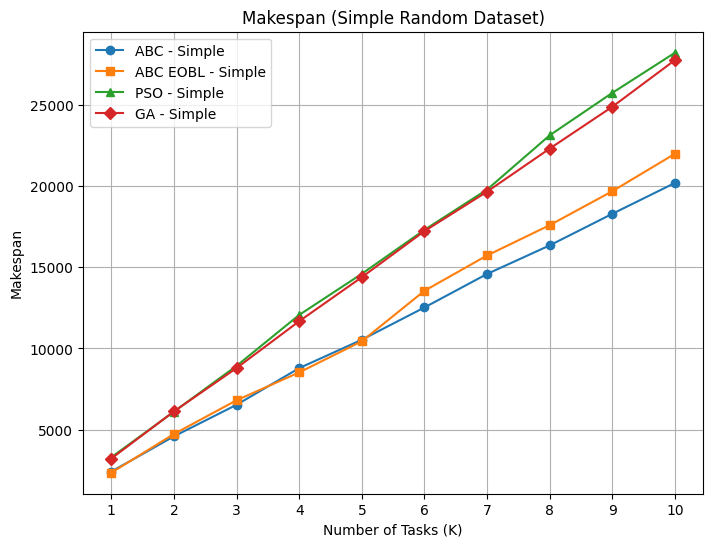
\includegraphics[width=0.75\linewidth]{gambar/Grafik Makespan Simple Random.png}
    \caption{Grafik \textit{makespan simple random}}
\end{figure}

\newpage

\begin{figure} [H]
    \centering
    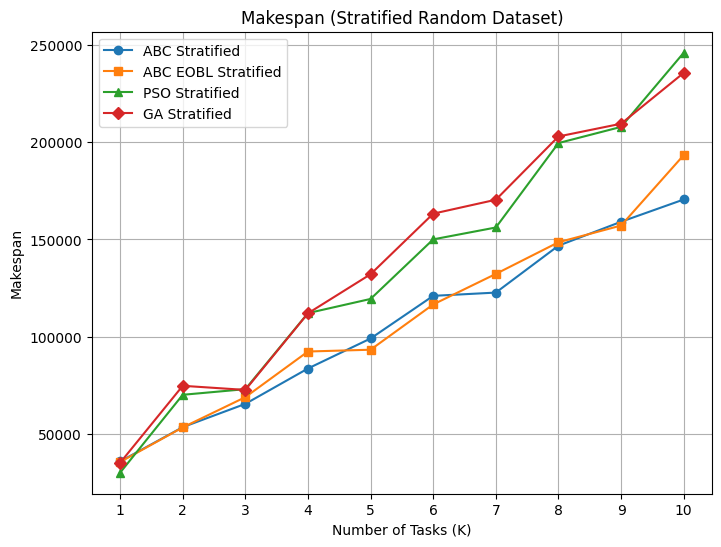
\includegraphics[width=0.75\linewidth]{gambar/Grafik Makespan Stratified Random.png}
    \caption{Grafik \textit{makespan stratified random}}
\end{figure}

\begin{figure} [H]
    \centering
    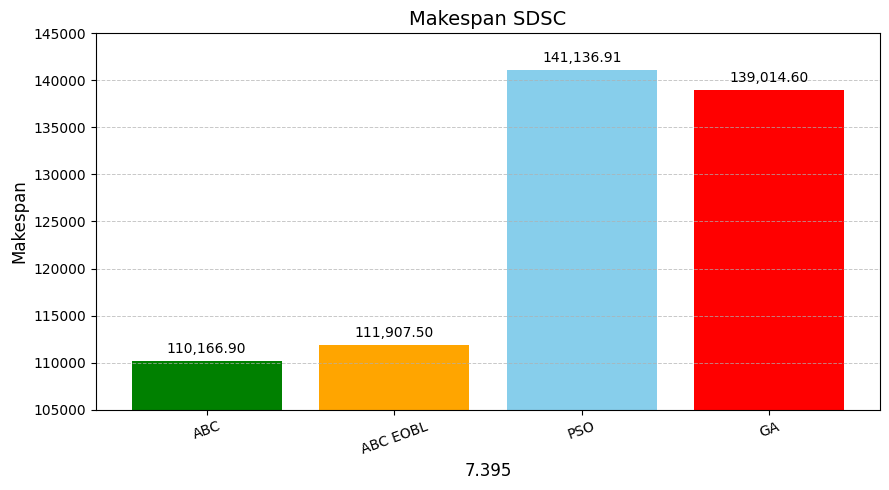
\includegraphics[width=0.75\linewidth]{gambar/Grafik Makespan SDSC.png}
    \caption{Grafik \textit{makespan} SDSC}
\end{figure}

\newpage

\begin{figure} [H]
    \centering
    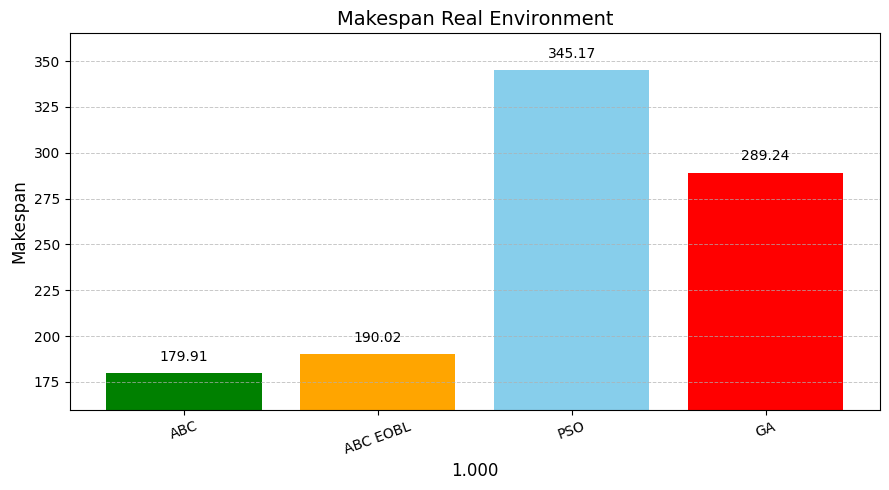
\includegraphics[width=0.75\linewidth]{gambar/Grafik Makespan Real Environment.png}
    \caption{Grafik \textit{makespan real environment}}
\end{figure}

\subsection{\textit{Average Start Time} (\textit{Lower Better})}
\textit{Average start time} mengacu pada waktu rata-rata yang diperlukan oleh algoritma untuk memulai eksekusi sebuah tugas pada lingkungan \textit{cloud}. Semakin rendah nilai \textit{average start time}, maka semakin baik kinerja algoritma tersebut dalam hal efisiensi waktu inisiasi tugas.

\begin{table} [H]
\centering
\caption{\textit{Average start time simple random}}
\begin{tabular}{|>{\raggedleft\arraybackslash}m{0.12\linewidth}|
                >{\raggedleft\arraybackslash}m{0.17\linewidth}|
                >{\raggedleft\arraybackslash}m{0.17\linewidth}|
                >{\raggedleft\arraybackslash}m{0.17\linewidth}|
                >{\raggedleft\arraybackslash}m{0.17\linewidth}|}
\rowcolor{blue!30}
\hline
\multicolumn{1}{|>{\centering\arraybackslash}m{0.12\linewidth}|}{\textbf{\textit{Cloudlets}}} & 
\multicolumn{1}{>{\centering\arraybackslash}m{0.17\linewidth}|}{\textbf{ABC \textit{Simple}}} & 
\multicolumn{1}{>{\centering\arraybackslash}m{0.17\linewidth}|}{\textbf{ABC EOBL \textit{Simple}}} & 
\multicolumn{1}{>{\centering\arraybackslash}m{0.17\linewidth}|}{\textbf{PSO \textit{Simple}}} & 
\multicolumn{1}{>{\centering\arraybackslash}m{0.17\linewidth}|}{\textbf{GA \textit{Simple}}} \\
\hline
1.000 & 738,30 & 732,27 & 1.008,53 & 1.097,42 \\
\hline
2.000 & 1.074,04 & 1.500,95 & 2.064,80 & 2.277,04 \\
\hline
3.000 & 2.246,88 & 2.245,16 & 3.056,15 & 3.380,23 \\
\hline
4.000 & 2.981,69 & 2.967,65 & 4.137,20 & 4.537,59 \\
\hline
5.000 & 3.700,48 & 3.676,07 & 5.142,45 & 5.597,77 \\
\hline
6.000 & 4.454,43 & 4.600,88 & 6.199,46 & 6.786,18 \\
\hline
7.000 & 5.200,75 & 5.380,87 & 7.153,93 & 7.863,54 \\
\hline
8.000 & 5.978,64 & 6.155,85 & 8.291,67 & 9.049,82 \\
\hline
9.000 & 6.714,10 & 6.910,13 & 9.288,67 & 10.157,47 \\
\hline
10.000 & 7.425,45 & 7.672,21 & 10.333,42 & 11.318,84 \\
\hline
\textbf{AVG} & \textcolor{green}{4.051,48} & 4.184,20 & 5.667,63 & 6.206,59 \\
\hline
\end{tabular}
\end{table}

\newpage

\begin{table} [H]
\centering
\caption{\textit{Average start time stratified random}}
\begin{tabular}{|>{\raggedleft\arraybackslash}m{0.12\linewidth}|
                >{\raggedleft\arraybackslash}m{0.17\linewidth}|
                >{\raggedleft\arraybackslash}m{0.17\linewidth}|
                >{\raggedleft\arraybackslash}m{0.17\linewidth}|
                >{\raggedleft\arraybackslash}m{0.17\linewidth}|}
\rowcolor{blue!30}
\hline
\multicolumn{1}{|>{\centering\arraybackslash}m{0.12\linewidth}|}{\textbf{\textit{Cloudlets}}} & 
\multicolumn{1}{>{\centering\arraybackslash}m{0.17\linewidth}|}{\textbf{ABC \textit{Stratified}}} & 
\multicolumn{1}{>{\centering\arraybackslash}m{0.17\linewidth}|}{\textbf{ABC EOBL \textit{Stratified}}} & 
\multicolumn{1}{>{\centering\arraybackslash}m{0.17\linewidth}|}{\textbf{PSO \textit{Stratified}}} & 
\multicolumn{1}{>{\centering\arraybackslash}m{0.17\linewidth}|}{\textbf{GA \textit{Stratified}}} \\
\hline
1.000 & 4.640,92 & 4.792,01 & 5.503,25 & 5.739,04 \\
\hline
2.000 & 10.177,47 & 10.785,78 & 14.849,58 & 16.087,73 \\
\hline
3.000 & 14.791,98 & 14.845,95 & 19.424,48 & 20.590,21 \\
\hline
4.000 & 20.742,34 & 21.314,79 & 28.380,60 & 32.214,32 \\
\hline
5.000 & 25.006,78 & 26.142,43 & 33.360,28 & 37.442,09 \\
\hline
6.000 & 31.639,72 & 31.604,86 & 43.449,62 & 48.034,96 \\
\hline
7.000 & 35.668,25 & 36.673,71 & 46.601,23 & 51.228,05 \\
\hline
8.000 & 41.471,38 & 43.314,06 & 58.719,59 & 63.714,31 \\
\hline
9.000 & 46.771,80 & 46.972,56 & 62.034,10 & 68.314,65 \\
\hline
10.000 & 51.402,64 & 54.759,20 & 72.289,93 & 79.753,82 \\
\hline
\textbf{AVG} & \textcolor{green}{28.231,33} & 29.120,54 & 38.461,27 & 42.311,92 \\
\hline
\end{tabular}
\end{table}

\begin{table} [H]
\centering
\caption{\textit{Average start time} SDSC}
\begin{tabular}{|>{\raggedleft\arraybackslash}m{0.12\linewidth}|
                >{\raggedleft\arraybackslash}m{0.15\linewidth}|
                >{\raggedleft\arraybackslash}m{0.25\linewidth}|
                >{\raggedleft\arraybackslash}m{0.15\linewidth}|
                >{\raggedleft\arraybackslash}m{0.15\linewidth}|}
\rowcolor{blue!30}
\hline
\multicolumn{1}{|>{\centering\arraybackslash}m{0.12\linewidth}|}{\textbf{\textit{Cloudlets}}} & 
\multicolumn{1}{>{\centering\arraybackslash}m{0.15\linewidth}|}{\textbf{ABC SDSC}} & 
\multicolumn{1}{>{\centering\arraybackslash}m{0.25\linewidth}|}{\textbf{ABC EOBL SDSC}} & 
\multicolumn{1}{>{\centering\arraybackslash}m{0.15\linewidth}|}{\textbf{PSO SDSC}} & 
\multicolumn{1}{>{\centering\arraybackslash}m{0.15\linewidth}|}{\textbf{GA SDSC}} \\
\hline
7.395 & \textcolor{green}{27.926,11} & 28.538,28 & 37.766,73 & 41.644,38\\
\hline
\end{tabular}
\end{table}

\begin{table} [H]
\centering
\caption{\textit{Average start time real environment}}
\begin{tabular}{|>{\raggedleft\arraybackslash}m{0.1\linewidth}|
                >{\raggedleft\arraybackslash}m{0.17\linewidth}|
                >{\raggedleft\arraybackslash}m{0.17\linewidth}|
                >{\raggedleft\arraybackslash}m{0.17\linewidth}|
                >{\raggedleft\arraybackslash}m{0.17\linewidth}|}
\rowcolor{blue!30}
\hline
\multicolumn{1}{|>{\centering\arraybackslash}m{0.1\linewidth}|}{\textbf{\textit{Task}}} & 
\multicolumn{1}{>{\centering\arraybackslash}m{0.17\linewidth}|}{\textbf{ABC RE}} & 
\multicolumn{1}{>{\centering\arraybackslash}m{0.17\linewidth}|}{\textbf{ABC EOBL RE}} & 
\multicolumn{1}{>{\centering\arraybackslash}m{0.17\linewidth}|}{\textbf{PSO RE}} & 
\multicolumn{1}{>{\centering\arraybackslash}m{0.17\linewidth}|}{\textbf{GA RE}} \\
\hline
1.000 & \textcolor{green}{89.620,01} & 92.554,11 & 196.952,51 & 144.562,97 \\
\hline
\end{tabular}
\end{table}

Berdasarkan hasil pengujian yang ditampilkan pada tabel dan grafik eksperimen, algoritma \textit{Artificial Bee Colony} (ABC) menunjukkan performa yang lebih baik dengan menghasilkan nilai \textit{average start time} paling rendah dibandingkan dengan algoritma ABC yang dikombinasikan dengan \textit{Elite Opposition-Based Learning} (ABC-EOBL). Hal ini konsisten terlihat pada \textit{dataset simple random}, \textit{stratified random}, maupun SDSC.

Penyebab utama meningkatnya nilai \textit{average start time} pada algoritma ABC-EOBL adalah kompleksitas tambahan yang dimiliki oleh pendekatan EOBL, terutama proses evaluasi solusi lawan yang secara signifikan menambah waktu komputasi. Kondisi ini menyebabkan waktu inisiasi eksekusi tugas menjadi lebih lama dibandingkan dengan algoritma ABC yang lebih sederhana, sehingga meningkatkan nilai \textit{average start time} pada ABC-EOBL.

\newpage

\begin{figure} [H]
    \centering
    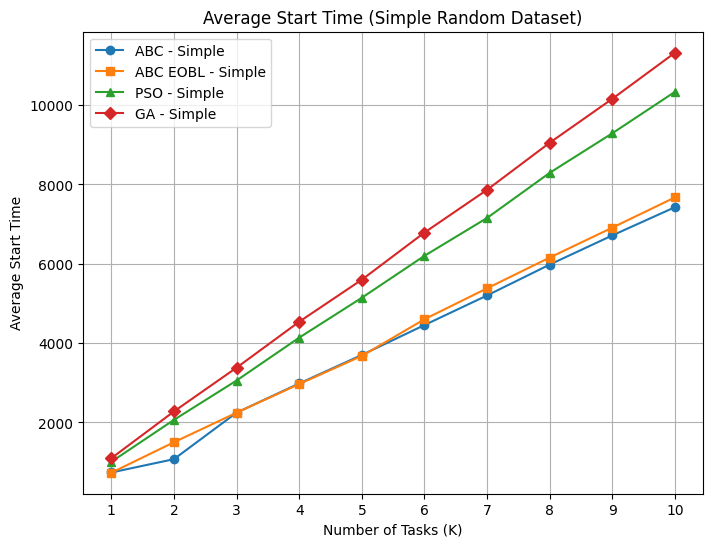
\includegraphics[width=0.75\linewidth]{gambar/Grafik Average Start Time Simple Random.png}
    \caption{Grafik \textit{average start time simple random}}
\end{figure}

\begin{figure} [H]
    \centering
    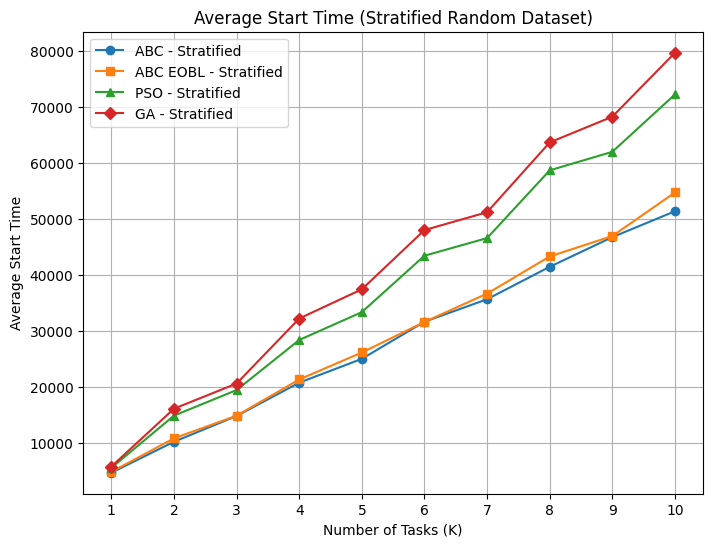
\includegraphics[width=0.75\linewidth]{gambar/Grafik Average Start Time Stratified Random.png}
    \caption{Grafik \textit{average start time stratified random}}
\end{figure}

\newpage

\begin{figure} [H]
    \centering
    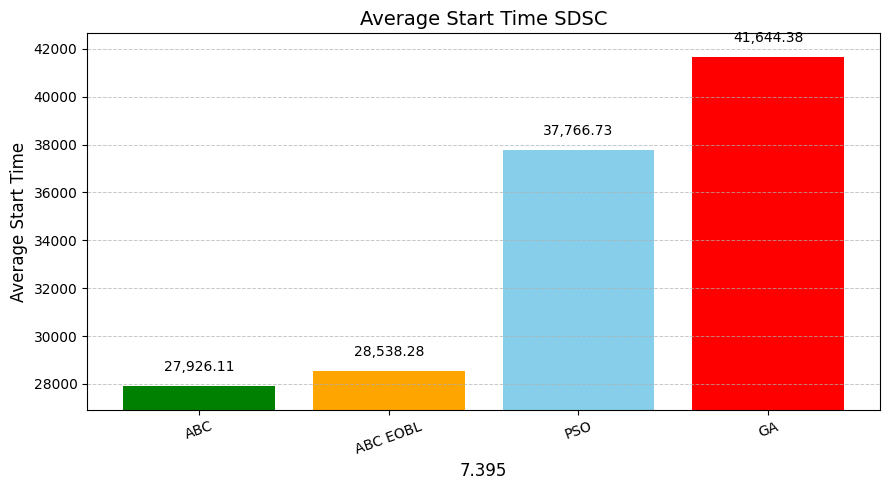
\includegraphics[width=0.75\linewidth]{gambar/Grafik Average Start Time SDSC.png}
    \caption{Grafik \textit{average start time} SDSC}
\end{figure}

\begin{figure} [H]
    \centering
    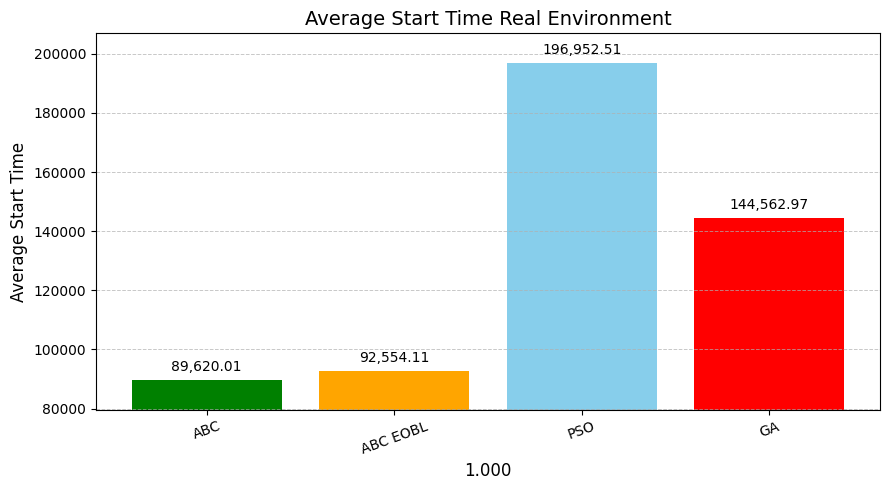
\includegraphics[width=0.75\linewidth]{gambar/Grafik Average Start Time Real Environment.png}
    \caption{Grafik \textit{average start time real environment}}
\end{figure}

\subsection{\textit{Average Finish Time} (\textit{Lower Better})}
\textit{Average finish time} adalah rata-rata waktu yang diperlukan oleh algoritma untuk menyelesaikan eksekusi suatu tugas pada lingkungan \textit{cloud}. Semakin rendah nilai \textit{average finish time}, semakin baik performa algoritma dalam hal efisiensi penyelesaian tugas.

\newpage

\begin{table} [H]
\centering
\caption{\textit{Average finish time simple random}}
\begin{tabular}{|>{\raggedleft\arraybackslash}m{0.12\linewidth}|
                >{\raggedleft\arraybackslash}m{0.17\linewidth}|
                >{\raggedleft\arraybackslash}m{0.17\linewidth}|
                >{\raggedleft\arraybackslash}m{0.17\linewidth}|
                >{\raggedleft\arraybackslash}m{0.17\linewidth}|}
\rowcolor{blue!30}
\hline
\multicolumn{1}{|>{\centering\arraybackslash}m{0.12\linewidth}|}{\textbf{\textit{Cloudlets}}} & 
\multicolumn{1}{>{\centering\arraybackslash}m{0.17\linewidth}|}{\textbf{ABC \textit{Simple}}} & 
\multicolumn{1}{>{\centering\arraybackslash}m{0.17\linewidth}|}{\textbf{ABC EOBL \textit{Simple}}} & 
\multicolumn{1}{>{\centering\arraybackslash}m{0.17\linewidth}|}{\textbf{PSO \textit{Simple}}} & 
\multicolumn{1}{>{\centering\arraybackslash}m{0.17\linewidth}|}{\textbf{GA \textit{Simple}}} \\
\hline
1.000 & 744,15 & 792,42 & 1.066,07 & 1.154,04 \\
\hline
2.000 & 1.155,26 & 1.560,74 & 2.121,92 & 2.333,22 \\
\hline
3.000 & 2.306,88 & 2.305,15 & 3.113,53 & 3.436,73 \\
\hline
4.000 & 3.041,32 & 3.027,39 & 4.194,14 & 4.593,67 \\
\hline
5.000 & 3.760,12 & 3.735,78 & 5.199,39 & 5.653,89 \\
\hline
6.000 & 4.514,15 & 4.660,33 & 6.256,46 & 6.842,31 \\
\hline
7.000 & 5.260,52 & 5.440,37 & 7.211,08 & 7.919,79 \\
\hline
8.000 & 6.038,45 & 6.215,45 & 8.348,82 & 9.106,11 \\
\hline
9.000 & 6.773,92 & 6.969,75 & 9.345,81 & 10.213,75 \\
\hline
10.000 & 7.485,23 & 7.731,69 & 10.390,46 & 11.375,02 \\
\hline
\textbf{AVG} & \textcolor{green}{4.108,00} & 4.243,91 & 5.724,77 & 6.262,85 \\
\hline
\end{tabular}
\end{table}

\begin{table} [H]
\centering
\caption{\textit{Average finish time stratified random}}
\begin{tabular}{|>{\raggedleft\arraybackslash}m{0.12\linewidth}|
                >{\raggedleft\arraybackslash}m{0.17\linewidth}|
                >{\raggedleft\arraybackslash}m{0.17\linewidth}|
                >{\raggedleft\arraybackslash}m{0.17\linewidth}|
                >{\raggedleft\arraybackslash}m{0.17\linewidth}|}
\rowcolor{blue!30}
\hline
\multicolumn{1}{|>{\centering\arraybackslash}m{0.12\linewidth}|}{\textbf{\textit{Cloudlets}}} & 
\multicolumn{1}{>{\centering\arraybackslash}m{0.17\linewidth}|}{\textbf{ABC \textit{Stratified}}} & 
\multicolumn{1}{>{\centering\arraybackslash}m{0.17\linewidth}|}{\textbf{ABC EOBL \textit{Stratified}}} & 
\multicolumn{1}{>{\centering\arraybackslash}m{0.17\linewidth}|}{\textbf{PSO \textit{Stratified}}} & 
\multicolumn{1}{>{\centering\arraybackslash}m{0.17\linewidth}|}{\textbf{GA \textit{Stratified}}} \\
\hline
1.000 & 5.129,75 & 5.269,51 & 5.973,21 & 6.209,89 \\
\hline
2.000 & 10.641,35 & 11.243,58 & 15.286,22 & 16.517,60 \\
\hline
3.000 & 15.266,41 & 15.322,64 & 19.881,74 & 21.040,78 \\
\hline
4.000 & 21.205,64 & 21.776,03 & 28.819,61 & 32.645,10 \\
\hline
5.000 & 25.477,13 & 26.611,62 & 33.812,72 & 37.883,78 \\
\hline
6.000 & 32.102,34 & 32.066,59 & 43.887,95 & 48.464,10 \\
\hline
7.000 & 36.135,94 & 37.140,14 & 47.049,03 & 51.667,85 \\
\hline
8.000 & 41.935,48 & 43.776,96 & 59.159,66 & 64.145,57 \\
\hline
9.000 & 47.237,64 & 47.440,02 & 62.480,53 & 68.752,49 \\
\hline
10.000 & 51.865,55 & 55.217,92 & 72.728,10 & 80.183,74 \\
\hline
\textbf{AVG} & \textcolor{green}{28.699,72} & 29.586,50 & 38.907,88 & 42.751,09 \\
\hline
\end{tabular}
\end{table}

\begin{table} [H]
\centering
\caption{\textit{Average finish time} SDSC}
\begin{tabular}{|>{\raggedleft\arraybackslash}m{0.12\linewidth}|
                >{\raggedleft\arraybackslash}m{0.15\linewidth}|
                >{\raggedleft\arraybackslash}m{0.25\linewidth}|
                >{\raggedleft\arraybackslash}m{0.15\linewidth}|
                >{\raggedleft\arraybackslash}m{0.15\linewidth}|}
\rowcolor{blue!30}
\hline
\multicolumn{1}{|>{\centering\arraybackslash}m{0.12\linewidth}|}{\textbf{\textit{Cloudlets}}} & 
\multicolumn{1}{>{\centering\arraybackslash}m{0.15\linewidth}|}{\textbf{ABC SDSC}} & 
\multicolumn{1}{>{\centering\arraybackslash}m{0.25\linewidth}|}{\textbf{ABC EOBL SDSC}} & 
\multicolumn{1}{>{\centering\arraybackslash}m{0.15\linewidth}|}{\textbf{PSO SDSC}} & 
\multicolumn{1}{>{\centering\arraybackslash}m{0.15\linewidth}|}{\textbf{GA SDSC}} \\
\hline
7.395 & \textcolor{green}{28.277,85} & 28.888,60 & 38.102,26 & 41.970,13 \\
\hline
\end{tabular}
\end{table}

\begin{table} [H]
\centering
\caption{\textit{Average finish time real environment}}
\begin{tabular}{|>{\raggedleft\arraybackslash}m{0.1\linewidth}|
                >{\raggedleft\arraybackslash}m{0.17\linewidth}|
                >{\raggedleft\arraybackslash}m{0.17\linewidth}|
                >{\raggedleft\arraybackslash}m{0.17\linewidth}|
                >{\raggedleft\arraybackslash}m{0.17\linewidth}|}
\rowcolor{blue!30}
\hline
\multicolumn{1}{|>{\centering\arraybackslash}m{0.1\linewidth}|}{\textbf{\textit{Task}}} & 
\multicolumn{1}{>{\centering\arraybackslash}m{0.17\linewidth}|}{\textbf{ABC RE}} & 
\multicolumn{1}{>{\centering\arraybackslash}m{0.17\linewidth}|}{\textbf{ABC EOBL RE}} & 
\multicolumn{1}{>{\centering\arraybackslash}m{0.17\linewidth}|}{\textbf{PSO RE}} & 
\multicolumn{1}{>{\centering\arraybackslash}m{0.17\linewidth}|}{\textbf{GA RE}} \\
\hline
1.000 & \textcolor{green}{89.783,92} & 92.722,07 & 197.276,29 & 144.789,12 \\
\hline
\end{tabular}
\end{table}

Berdasarkan hasil pengujian pada tabel dan grafik eksperimen, algoritma \textit{Artificial Bee Colony} (ABC) menunjukkan nilai \textit{average finish time} paling rendah secara konsisten dibandingkan dengan algoritma ABC yang dikombinasikan dengan \textit{Elite Opposition-Based Learning} (EOBL). Pada \textit{dataset simple random}, ABC secara jelas menunjukkan performa terbaik dengan waktu penyelesaian rata-rata yang lebih cepat dibandingkan ABC-EOBL. Kondisi serupa juga terlihat pada \textit{dataset stratified random}, di mana ABC tanpa modifikasi mampu menyelesaikan tugas lebih efisien dibandingkan dengan algoritma ABC-EOBL.

Penyebab utama nilai \textit{average finish time} yang lebih tinggi pada algoritma ABC-EOBL adalah kompleksitas tambahan dari metode \textit{Elite Opposition-Based Learning}. Metode ini memerlukan evaluasi tambahan terhadap solusi lawan, yang menyebabkan waktu komputasi lebih lama dan memperlambat konvergensi menuju solusi optimal. Akibatnya, algoritma membutuhkan waktu lebih lama untuk menyelesaikan eksekusi tugas.

\begin{figure} [H]
    \centering
    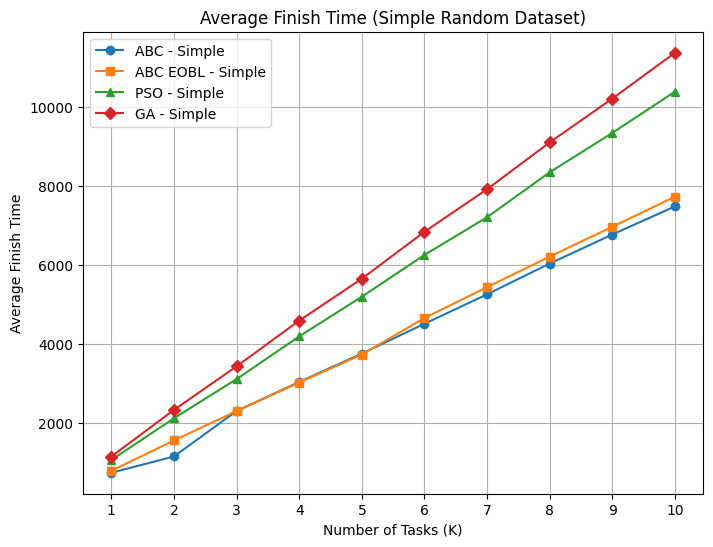
\includegraphics[width=0.75\linewidth]{gambar/Grafik Average Finish Time Simple Random.png}
    \caption{Grafik \textit{average finish time simple random}}
\end{figure}

\newpage

\begin{figure} [H]
    \centering
    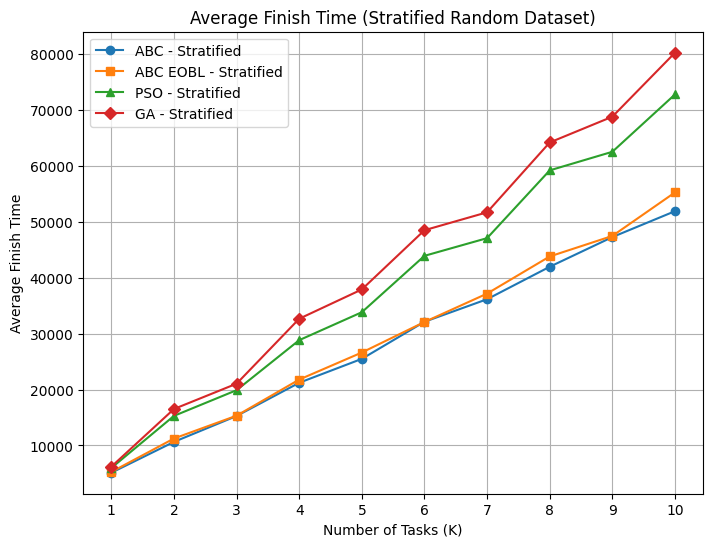
\includegraphics[width=0.75\linewidth]{gambar/Grafik Average Finish Time Stratified Random.png}
    \caption{Grafik \textit{average finish time stratified random}}
\end{figure}

\begin{figure} [H]
    \centering
    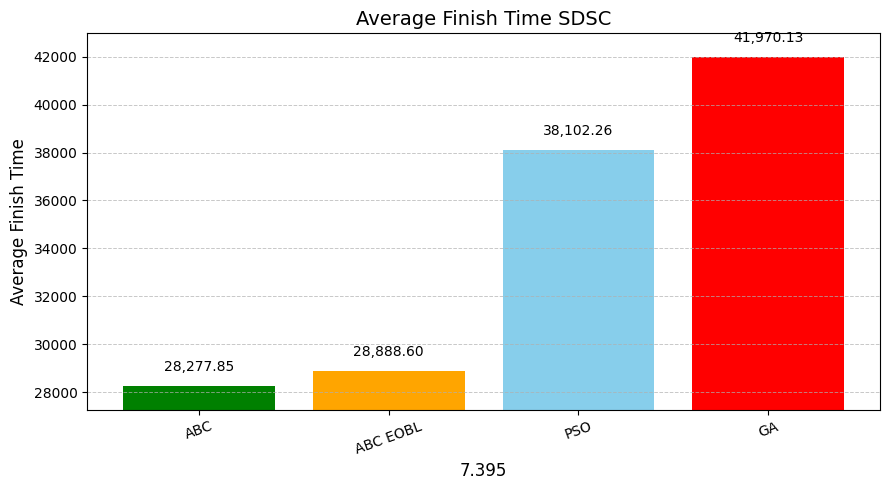
\includegraphics[width=0.75\linewidth]{gambar/Grafik Average Finish Time SDSC.png}
    \caption{Grafik \textit{average finish time} SDSC}
\end{figure}

\newpage

\begin{figure} [H]
    \centering
    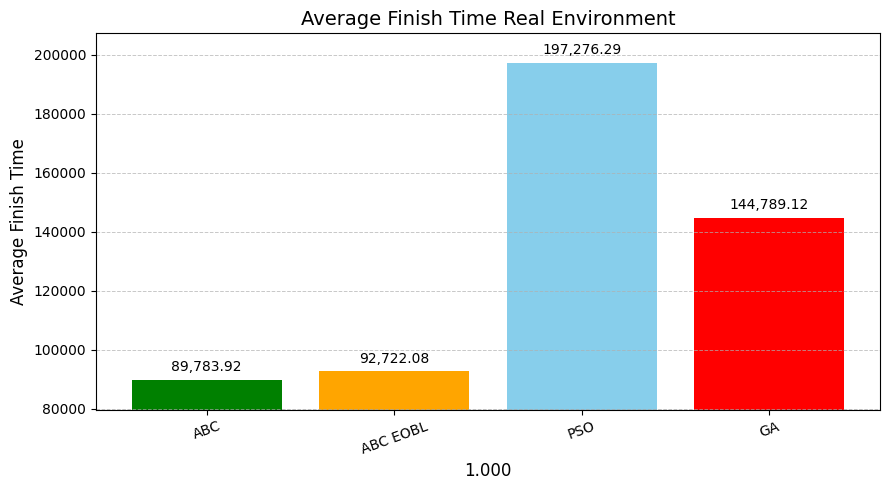
\includegraphics[width=0.75\linewidth]{gambar/Grafik Average Finish Time Real Environment.png}
    \caption{Grafik \textit{average finish time real environment}}
\end{figure}

\subsection{\textit{Average Execution Time} (\textit{Lower Better})}
\textit{Average execution time} merujuk pada waktu rata-rata yang dibutuhkan algoritma untuk menyelesaikan proses eksekusi sebuah tugas pada lingkungan \textit{cloud}. Semakin rendah nilai \textit{average execution time}, semakin baik efisiensi algoritma dalam menjalankan tugas-tugas tersebut.

\begin{table} [H]
\centering
\caption{\textit{Average execution time simple random}}
\begin{tabular}{|>{\raggedleft\arraybackslash}m{0.12\linewidth}|
                >{\raggedleft\arraybackslash}m{0.17\linewidth}|
                >{\raggedleft\arraybackslash}m{0.17\linewidth}|
                >{\raggedleft\arraybackslash}m{0.17\linewidth}|
                >{\raggedleft\arraybackslash}m{0.17\linewidth}|}
\rowcolor{blue!30}
\hline
\multicolumn{1}{|>{\centering\arraybackslash}m{0.12\linewidth}|}{\textbf{\textit{Cloudlets}}} & 
\multicolumn{1}{>{\centering\arraybackslash}m{0.17\linewidth}|}{\textbf{ABC \textit{Simple}}} & 
\multicolumn{1}{>{\centering\arraybackslash}m{0.17\linewidth}|}{\textbf{ABC EOBL \textit{Simple}}} & 
\multicolumn{1}{>{\centering\arraybackslash}m{0.17\linewidth}|}{\textbf{PSO \textit{Simple}}} & 
\multicolumn{1}{>{\centering\arraybackslash}m{0.17\linewidth}|}{\textbf{GA \textit{Simple}}} \\
\hline
1.000 & 59,90 & 60,15 & 57,54 & 56,62 \\
\hline
2.000 & 59,70 & 59,79 & 57,12 & 56,19 \\
\hline
3.000 & 60,00 & 59,99 & 57,38 & 56,49 \\
\hline
4.000 & 59,62 & 59,74 & 56,94 & 56,08 \\
\hline
5.000 & 59,64 & 59,71 & 56,94 & 56,12 \\
\hline
6.000 & 59,71 & 59,45 & 57,00 & 56,13 \\
\hline
7.000 & 59,78 & 59,50 & 57,15 & 56,25 \\
\hline
8.000 & 59,81 & 59,59 & 57,16 & 56,29 \\
\hline
9.000 & 59,82 & 59,61 & 57,15 & 56,28 \\
\hline
10.000 & 59,78 & 59,48 & 57,04 & 56,17 \\
\hline
\textbf{AVG} & 59,78 & 59,70 & 57,14 & \textcolor{green}{56,26} \\
\hline
\end{tabular}
\end{table}

\newpage

\begin{table} [H]
\centering
\caption{\textit{Average execution time stratified random}}
\begin{tabular}{|>{\raggedleft\arraybackslash}m{0.12\linewidth}|
                >{\raggedleft\arraybackslash}m{0.17\linewidth}|
                >{\raggedleft\arraybackslash}m{0.17\linewidth}|
                >{\raggedleft\arraybackslash}m{0.17\linewidth}|
                >{\raggedleft\arraybackslash}m{0.17\linewidth}|}
\rowcolor{blue!30}
\hline
\multicolumn{1}{|>{\centering\arraybackslash}m{0.12\linewidth}|}{\textbf{\textit{Cloudlets}}} & 
\multicolumn{1}{>{\centering\arraybackslash}m{0.17\linewidth}|}{\textbf{ABC \textit{Stratified}}} & 
\multicolumn{1}{>{\centering\arraybackslash}m{0.17\linewidth}|}{\textbf{ABC EOBL \textit{Stratified}}} & 
\multicolumn{1}{>{\centering\arraybackslash}m{0.17\linewidth}|}{\textbf{PSO \textit{Stratified}}} & 
\multicolumn{1}{>{\centering\arraybackslash}m{0.17\linewidth}|}{\textbf{GA \textit{Stratified}}} \\
\hline
1.000 & 488,83 & 477,50 & 469,97 & 470,85 \\
\hline
2.000 & 463,88 & 457,80 & 436,64 & 429,87 \\
\hline
3.000 & 474,44 & 476,69 & 457,27 & 450,56 \\
\hline
4.000 & 463,30 & 461,25 & 439,00 & 430,78 \\
\hline
5.000 & 470,35 & 469,19 & 452,44 & 441,69 \\
\hline
6.000 & 462,62 & 461,73 & 438,33 & 429,15 \\
\hline
7.000 & 467,69 & 466,43 & 447,79 & 439,80 \\
\hline
8.000 & 464,10 & 462,90 & 440,07 & 431,27 \\
\hline
9.000 & 465,85 & 467,46 & 446,43 & 437,84 \\
\hline
10.000 & 462,91 & 458,73 & 438,17 & 429,92 \\
\hline
\textbf{AVG} & 468,40 & 465,97 & 446,61 & \textcolor{green}{439,17} \\
\hline
\end{tabular}
\end{table}

\begin{table} [H]
\centering
\caption{\textit{Average execution time} SDSC}
\begin{tabular}{|>{\raggedleft\arraybackslash}m{0.12\linewidth}|
                >{\raggedleft\arraybackslash}m{0.15\linewidth}|
                >{\raggedleft\arraybackslash}m{0.25\linewidth}|
                >{\raggedleft\arraybackslash}m{0.15\linewidth}|
                >{\raggedleft\arraybackslash}m{0.15\linewidth}|}
\rowcolor{blue!30}
\hline
\multicolumn{1}{|>{\centering\arraybackslash}m{0.12\linewidth}|}{\textbf{Cloudlets}} & 
\multicolumn{1}{>{\centering\arraybackslash}m{0.15\linewidth}|}{\textbf{ABC SDSC}} & 
\multicolumn{1}{>{\centering\arraybackslash}m{0.25\linewidth}|}{\textbf{ABC EOBL SDSC}} & 
\multicolumn{1}{>{\centering\arraybackslash}m{0.15\linewidth}|}{\textbf{PSO SDSC}} & 
\multicolumn{1}{>{\centering\arraybackslash}m{0.15\linewidth}|}{\textbf{GA SDSC}} \\
\hline
7.395 & 351,73 & 350,31 & 335,53 & \textcolor{green}{325,75} \\
\hline
\end{tabular}
\end{table}

\begin{table} [H]
\centering
\caption{\textit{Average execution time real environment}}
\begin{tabular}{|>{\raggedleft\arraybackslash}m{0.1\linewidth}|
                >{\raggedleft\arraybackslash}m{0.17\linewidth}|
                >{\raggedleft\arraybackslash}m{0.17\linewidth}|
                >{\raggedleft\arraybackslash}m{0.17\linewidth}|
                >{\raggedleft\arraybackslash}m{0.17\linewidth}|}
\rowcolor{blue!30}
\hline
\multicolumn{1}{|>{\centering\arraybackslash}m{0.1\linewidth}|}{\textbf{\textit{Task}}} & 
\multicolumn{1}{>{\centering\arraybackslash}m{0.17\linewidth}|}{\textbf{ABC RE}} & 
\multicolumn{1}{>{\centering\arraybackslash}m{0.17\linewidth}|}{\textbf{ABC EOBL RE}} & 
\multicolumn{1}{>{\centering\arraybackslash}m{0.17\linewidth}|}{\textbf{PSO RE}} & 
\multicolumn{1}{>{\centering\arraybackslash}m{0.17\linewidth}|}{\textbf{GA RE}} \\
\hline
1.000 & \textcolor{green}{163,91} & 167,966 & 323,78 & 226.15 \\
\hline
\end{tabular}
\end{table}

Berdasarkan hasil eksperimen yang disajikan dalam tabel dan grafik, terlihat bahwa Genetic Algorithm (GA) secara konsisten menunjukkan nilai Average Execution Time terendah pada seluruh dataset yang diuji, mengindikasikan efisiensi eksekusi tugas yang paling tinggi dibandingkan algoritma lainnya. Kemudian, algoritma Artificial Bee Colony dengan Elite Opposition-Based Learning (ABC-EOBL) menempati posisi ketiga setelah Particle Swarm Optimization (PSO), dengan waktu eksekusi rata-rata yang sedikit lebih tinggi dibandingkan PSO namun lebih rendah daripada algoritma ABC.

Algoritma ABC memiliki nilai Average Execution Time tertinggi, menunjukkan bahwa algoritma ini membutuhkan waktu paling lama dalam menyelesaikan eksekusi tugas. Penyebab utama dari perbedaan ini adalah algoritma ABC yang tidak memiliki mekanisme pencarian adaptif seefisien GA dan PSO ataupun mekanisme diversifikasi solusi yang dimiliki ABC-EOBL, sehingga proses pencarian solusi optimal menjadi lebih lama.

\newpage

\begin{figure} [H]
    \centering
    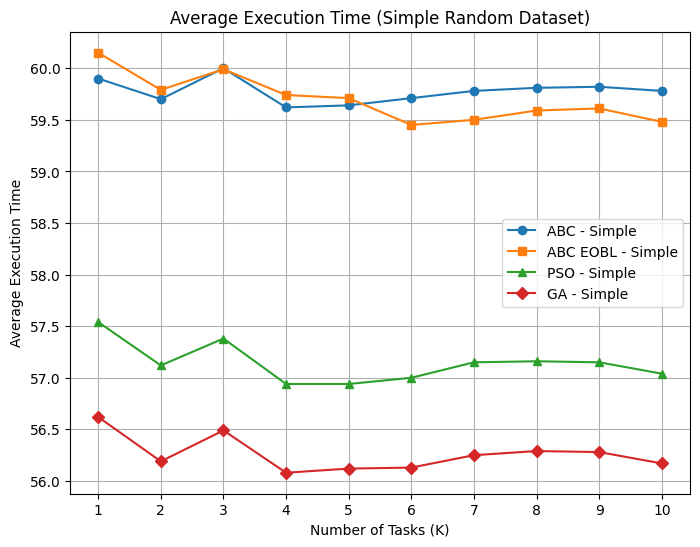
\includegraphics[width=0.75\linewidth]{gambar/Grafik Average Execution Time Simple Random.png}
    \caption{Grafik \textit{average execution time simple random}}
\end{figure}

\begin{figure} [H]
    \centering
    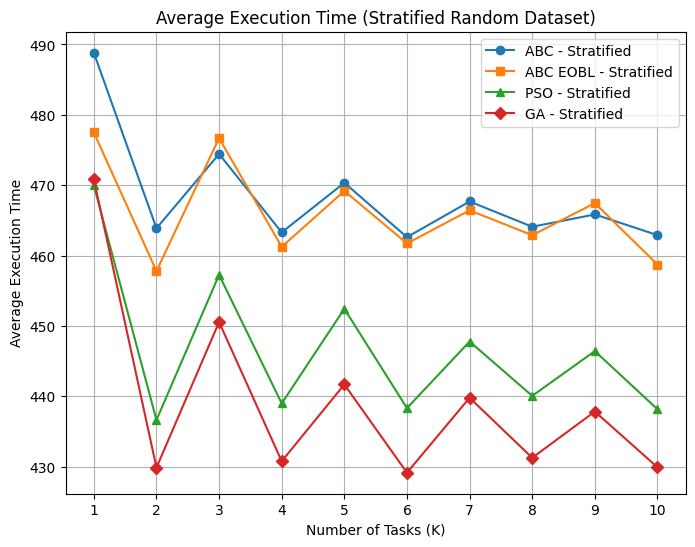
\includegraphics[width=0.75\linewidth]{gambar/Grafik Average Execution Time Stratified Random.png}
    \caption{Grafik \textit{average execution time stratified random}}
\end{figure}

\newpage

\begin{figure} [H]
    \centering
    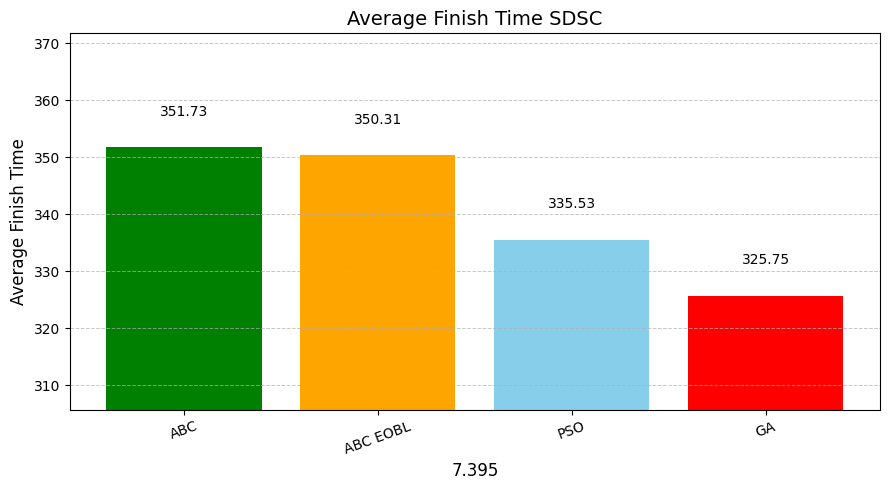
\includegraphics[width=0.75\linewidth]{gambar/Grafik Average Execution Time SDSC.png}
    \caption{Grafik \textit{average execution time} SDSC}
\end{figure}

\begin{figure} [H]
    \centering
    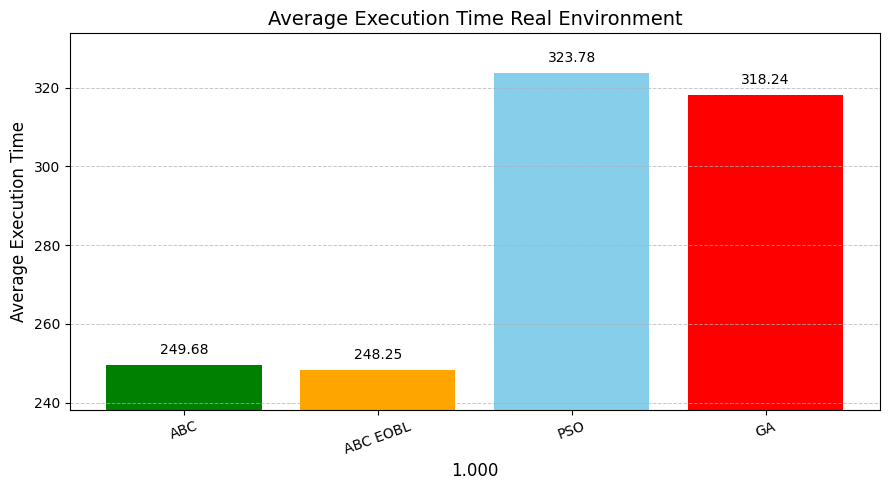
\includegraphics[width=0.75\linewidth]{gambar/Grafik Average Execution Time Real Environment.png}
    \caption{Grafik \textit{average execution time real environment}}
\end{figure}

\subsection{\textit{Average Waiting Time} (\textit{Lower Better})}
\textit{Average waiting time} mengacu pada waktu rata-rata yang dihabiskan oleh setiap tugas dalam antrian sebelum diproses oleh \textit{virtual machine}. Semakin rendah nilai \textit{average waiting time}, maka semakin efisien algoritma dalam mengatur dan mendistribusikan penjadwalan tugas.

\newpage

\begin{table} [H]
\centering
\caption{Average waiting time simple random}
\begin{tabular}{|>{\raggedleft\arraybackslash}m{0.12\linewidth}|
                >{\raggedleft\arraybackslash}m{0.17\linewidth}|
                >{\raggedleft\arraybackslash}m{0.17\linewidth}|
                >{\raggedleft\arraybackslash}m{0.17\linewidth}|
                >{\raggedleft\arraybackslash}m{0.17\linewidth}|}
\rowcolor{blue!30}
\hline
\multicolumn{1}{|>{\centering\arraybackslash}m{0.12\linewidth}|}{\textbf{\textit{Cloudlets}}} & 
\multicolumn{1}{>{\centering\arraybackslash}m{0.17\linewidth}|}{\textbf{ABC \textit{Simple}}} & 
\multicolumn{1}{>{\centering\arraybackslash}m{0.17\linewidth}|}{\textbf{ABC EOBL \textit{Simple}}} & 
\multicolumn{1}{>{\centering\arraybackslash}m{0.17\linewidth}|}{\textbf{PSO \textit{Simple}}} & 
\multicolumn{1}{>{\centering\arraybackslash}m{0.17\linewidth}|}{\textbf{GA \textit{Simple}}} \\
\hline
1.000 & 2,34 & 2,27 & 3,24 & 3,16 \\
\hline
2.000 & 2,26 & 2,34 & 3,02 & 3,03 \\
\hline
3.000 & 2,15 & 2,25 & 2,95 & 2,91 \\
\hline
4.000 & 2,18 & 2,12 & 3,00 & 2,91 \\
\hline
5.000 & 2,10 & 2,08 & 2,91 & 2,87 \\
\hline
6.000 & 2,08 & 2,25 & 2,87 & 2,86 \\
\hline
7.000 & 2,08 & 2,24 & 2,82 & 2,80 \\
\hline
8.000 & 2,04 & 2,19 & 2,88 & 2,78 \\
\hline
9.000 & 2,03 & 2,18 & 2,85 & 2,76 \\
\hline
10.000 & 2,02 & 2,19 & 2,82 & 2,77 \\
\hline
\textbf{AVG} & \textcolor{green}{2,13} & 2,21 & 2,94 & 2,89 \\
\hline
\end{tabular}
\end{table}

\begin{table} [H]
\centering
\caption{\textit{Average waiting time stratified random}}
\begin{tabular}{|>{\raggedleft\arraybackslash}m{0.12\linewidth}|
                >{\raggedleft\arraybackslash}m{0.17\linewidth}|
                >{\raggedleft\arraybackslash}m{0.17\linewidth}|
                >{\raggedleft\arraybackslash}m{0.17\linewidth}|
                >{\raggedleft\arraybackslash}m{0.17\linewidth}|}
\rowcolor{blue!30}
\hline
\multicolumn{1}{|>{\centering\arraybackslash}m{0.12\linewidth}|}{\textbf{\textit{Cloudlets}}} & 
\multicolumn{1}{>{\centering\arraybackslash}m{0.17\linewidth}|}{\textbf{ABC \textit{Stratified}}} & 
\multicolumn{1}{>{\centering\arraybackslash}m{0.17\linewidth}|}{\textbf{ABC EOBL \textit{Stratified}}} & 
\multicolumn{1}{>{\centering\arraybackslash}m{0.17\linewidth}|}{\textbf{PSO \textit{Stratified}}} & 
\multicolumn{1}{>{\centering\arraybackslash}m{0.17\linewidth}|}{\textbf{GA \textit{Stratified}}} \\
\hline
1.000 & 33,91 & 33,64 & 29,14 & 27,68 \\
\hline
2.000 & 26,73 & 26,02 & 34,98 & 37,38 \\
\hline
3.000 & 21,56 & 22,70 & 23,99 & 24,00 \\
\hline
4.000 & 20,79 & 22,95 & 28,01 & 28,00 \\
\hline
5.000 & 19,65 & 18,57 & 23,87 & 26,16 \\
\hline
6.000 & 20,16 & 19,27 & 24,99 & 27,07 \\
\hline
7.000 & 17,46 & 18,88 & 21,85 & 24,24 \\
\hline
8.000 & 18,34 & 18,56 & 24,91 & 25,28 \\
\hline
9.000 & 17,67 & 17,40 & 23,04 & 23,25 \\
\hline
10.000 & 17,01 & 19,30 & 24,58 & 23,53 \\
\hline
\textbf{AVG} & \textcolor{green}{21,33} & 21,73 & 25,94 & 26,66 \\
\hline
\end{tabular}
\end{table}

\begin{table} [H]
\centering
\caption{\textit{Average waiting time} SDSC}
\begin{tabular}{|>{\raggedleft\arraybackslash}m{0.12\linewidth}|
                >{\raggedleft\arraybackslash}m{0.15\linewidth}|
                >{\raggedleft\arraybackslash}m{0.25\linewidth}|
                >{\raggedleft\arraybackslash}m{0.15\linewidth}|
                >{\raggedleft\arraybackslash}m{0.15\linewidth}|}
\rowcolor{blue!30}
\hline
\multicolumn{1}{|>{\centering\arraybackslash}m{0.12\linewidth}|}{\textbf{\textit{Cloudlets}}} & 
\multicolumn{1}{>{\centering\arraybackslash}m{0.15\linewidth}|}{\textbf{ABC SDSC}} & 
\multicolumn{1}{>{\centering\arraybackslash}m{0.25\linewidth}|}{\textbf{ABC EOBL SDSC}} & 
\multicolumn{1}{>{\centering\arraybackslash}m{0.15\linewidth}|}{\textbf{PSO SDSC}} & 
\multicolumn{1}{>{\centering\arraybackslash}m{0.15\linewidth}|}{\textbf{GA SDSC}} \\
\hline
7.395 & \textcolor{green}{14,81} & 15,12 & 19,05 & 18,65 \\
\hline
\end{tabular}
\end{table}

\begin{table} [H]
\centering
\caption{\textit{Average waiting time real environment}}
\begin{tabular}{|>{\raggedleft\arraybackslash}m{0.1\linewidth}|
                >{\raggedleft\arraybackslash}m{0.17\linewidth}|
                >{\raggedleft\arraybackslash}m{0.17\linewidth}|
                >{\raggedleft\arraybackslash}m{0.17\linewidth}|
                >{\raggedleft\arraybackslash}m{0.17\linewidth}|}
\rowcolor{blue!30}
\hline
\multicolumn{1}{|>{\centering\arraybackslash}m{0.1\linewidth}|}{\textbf{\textit{Task}}} & 
\multicolumn{1}{>{\centering\arraybackslash}m{0.17\linewidth}|}{\textbf{ABC RE}} & 
\multicolumn{1}{>{\centering\arraybackslash}m{0.17\linewidth}|}{\textbf{ABC EOBL RE}} & 
\multicolumn{1}{>{\centering\arraybackslash}m{0.17\linewidth}|}{\textbf{PSO RE}} & 
\multicolumn{1}{>{\centering\arraybackslash}m{0.17\linewidth}|}{\textbf{GA RE}} \\
\hline
1.000 & \textcolor{green}{89.604,01} & 92.532,06 & 196.931,12 & 144.499,88 \\
\hline
\end{tabular}
\end{table}

Berdasarkan hasil eksperimen yang disajikan pada tabel dan grafik, algoritma \textit{Artificial Bee Colony} (ABC) secara konsisten menunjukkan nilai \textit{average waiting time} paling rendah pada seluruh \textit{dataset} yang diuji, baik pada \textit{simple random}, \textit{stratified random}, maupun SDSC. Hal ini menunjukkan bahwa ABC memiliki efisiensi tertinggi dalam mengurangi waktu tunggu rata-rata setiap tugas sebelum diproses.

Algoritma ABC dengan \textit{Elite Opposition-Based Learning} (EOBL) menempati posisi kedua, dengan nilai \textit{average waiting time} yang sedikit lebih tinggi dibandingkan ABC, namun tetap lebih baik dibandingkan dengan \textit{Particle Swarm Optimization} (PSO) maupun \textit{Genetic Algorithm} (GA). PSO justru memiliki nilai \textit{average waiting time} tertinggi, diikuti oleh GA pada \textit{dataset} SDSC, sedangkan GA memiliki nilai \textit{average waiting time} tertinggi pada \textit{dataset simple random} dan \textit{stratified random}.

Penyebab utama rendahnya \textit{average waiting time} pada ABC adalah kesederhanaan proses penjadwalan dan kecenderungan algoritma ini untuk langsung mendistribusikan tugas secara optimal tanpa tambahan proses komputasi yang kompleks. Sementara itu, tambahan mekanisme pada ABC-EOBL, dapat menambah beban komputasi, yang menyebabkan akumulasi waktu tunggu yang lebih tinggi.

\begin{figure} [H]
    \centering
    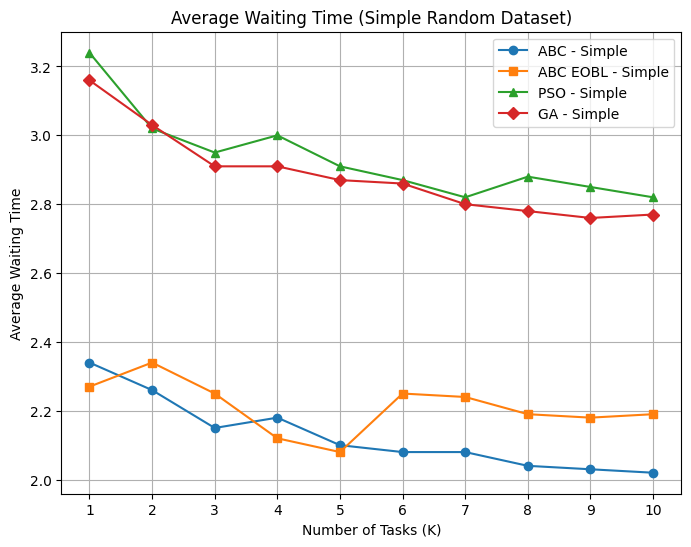
\includegraphics[width=0.75\linewidth]{gambar/Grafik Average Waiting Time Simple Random.png}
    \caption{Grafik \textit{average waiting time simple random}}
\end{figure}

\newpage

\begin{figure} [H]
    \centering
    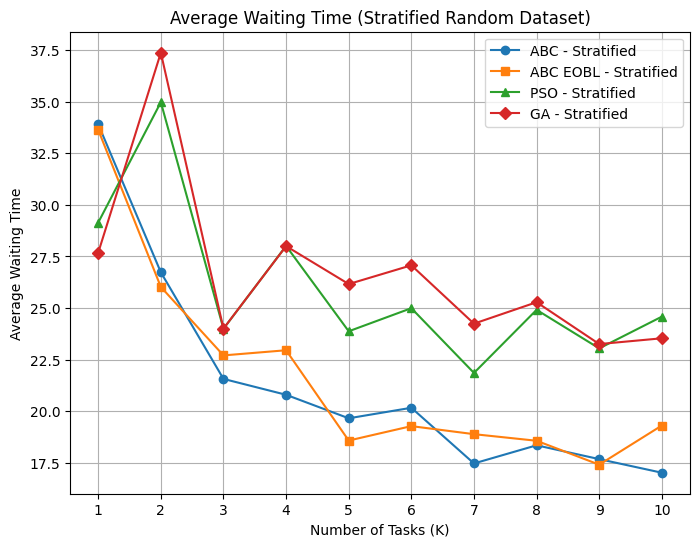
\includegraphics[width=0.75\linewidth]{gambar/Grafik Average Waiting Time Stratified Random.png}
    \caption{Grafik \textit{average waiting time stratified random}}
\end{figure}

\begin{figure} [H]
    \centering
    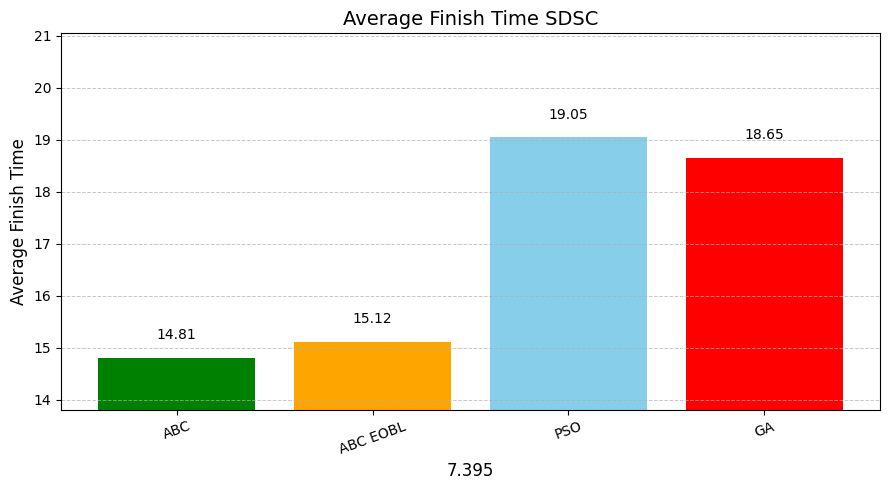
\includegraphics[width=0.75\linewidth]{gambar/Grafik Average Waiting Time SDSC.png}
    \caption{Grafik \textit{average waiting time} SDSC}
\end{figure}

\newpage

\begin{figure} [H]
    \centering
    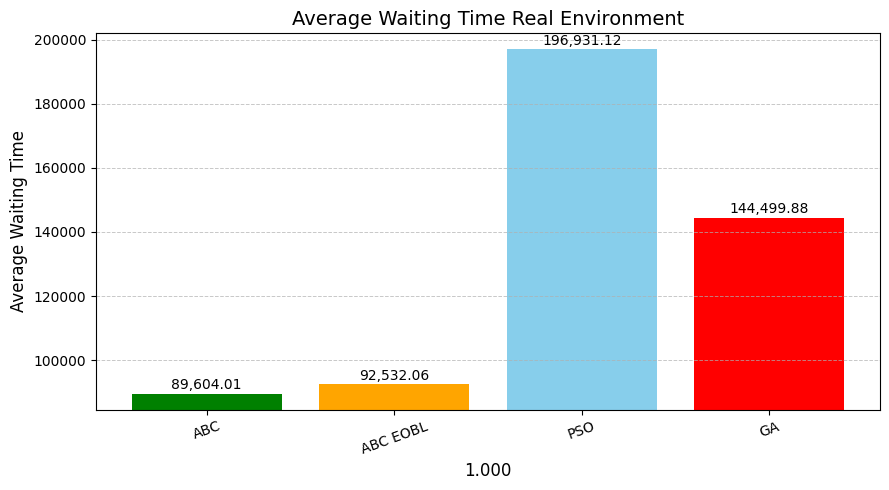
\includegraphics[width=0.75\linewidth]{gambar/Grafik Average Waiting Time Real Environment.png}
    \caption{Grafik \textit{average waiting rime real environment}}
\end{figure}

\subsection{\textit{Scheduling Length} (\textit{Lower Better})}
\textit{Scheduling length} adalah waktu keseluruhan yang diperlukan untuk menyelesaikan seluruh proses penjadwalan dan simulasi \textit{cloud} dari awal hingga akhir. Semakin rendah nilai \textit{scheduling length}, semakin efisien algoritma dalam menyelesaikan seluruh rangkaian tugas yang dijadwalkan.

\begin{table} [H]
\centering
\caption{\textit{Scheduling length simple random}}
\begin{tabular}{|>{\raggedleft\arraybackslash}m{0.12\linewidth}|
                >{\raggedleft\arraybackslash}m{0.17\linewidth}|
                >{\raggedleft\arraybackslash}m{0.17\linewidth}|
                >{\raggedleft\arraybackslash}m{0.17\linewidth}|
                >{\raggedleft\arraybackslash}m{0.17\linewidth}|}
\rowcolor{blue!30}
\hline
\multicolumn{1}{|>{\centering\arraybackslash}m{0.12\linewidth}|}{\textbf{\textit{Cloudlets}}} & 
\multicolumn{1}{>{\centering\arraybackslash}m{0.17\linewidth}|}{\textbf{ABC \textit{Simple}}} & 
\multicolumn{1}{>{\centering\arraybackslash}m{0.17\linewidth}|}{\textbf{ABC EOBL \textit{Simple}}} & 
\multicolumn{1}{>{\centering\arraybackslash}m{0.17\linewidth}|}{\textbf{PSO \textit{Simple}}} & 
\multicolumn{1}{>{\centering\arraybackslash}m{0.17\linewidth}|}{\textbf{GA \textit{Simple}}} \\
\hline
1.000 & 743.400,60 & 734.004,60 & 1.011.223,50 & 1.100.030,10 \\
\hline
2.000 & 2.989.205,70 & 3.005.431,80 & 4.134.511,50 & 4.558.990,20 \\
\hline
3.000 & 6.745.376,40 & 6.740.484,00 & 9.175.560,90 & 10.147.693,20 \\
\hline
4.000 & 11.933.167,20 & 11.876.727,30 & 16.558.460,70 & 18.159.654,30 \\
\hline
5.000 & 18.509.958,60 & 18.387.784,50 & 25.723.842,00 & 28.000.251,60 \\
\hline
6.000 & 26.735.547,30 & 27.615.263,10 & 37.210.486,20 & 40.730.730,90 \\
\hline
7.000 & 36.415.642,20 & 37.677.615,00 & 50.093.097,90 & 55.060.249,20 \\
\hline
8.000 & 47.840.731,80 & 49.259.633,10 & 66.351.669,00 & 72.416.049,00 \\
\hline
9.000 & 60.439.857,00 & 62.205.504,00 & 83.618.349,00 & 91.436.716,50 \\
\hline
10.000 & 74.268.742,20 & 76.738.122,60 & 103.356.471,30 & 113.210.187,00 \\
\hline
\textbf{AVG} & \textcolor{green}{28.662.162,90} & 29.424.057,00 & 39.723.367,20 & 43.482.055,20 \\
\hline
\end{tabular}
\end{table}

\newpage

\begin{table} [H]
\centering
\caption{\textit{Scheduling length stratified random}}
\begin{tabular}{|>{\raggedleft\arraybackslash}m{0.12\linewidth}|
                >{\raggedleft\arraybackslash}m{0.17\linewidth}|
                >{\raggedleft\arraybackslash}m{0.17\linewidth}|
                >{\raggedleft\arraybackslash}m{0.17\linewidth}|
                >{\raggedleft\arraybackslash}m{0.17\linewidth}|}
\rowcolor{blue!30}
\hline
\multicolumn{1}{|>{\centering\arraybackslash}m{0.12\linewidth}|}{\textbf{\textit{Cloudlets}}} & 
\multicolumn{1}{>{\centering\arraybackslash}m{0.17\linewidth}|}{\textbf{ABC \textit{Stratified}}} & 
\multicolumn{1}{>{\centering\arraybackslash}m{0.17\linewidth}|}{\textbf{ABC EOBL \textit{Stratified}}} & 
\multicolumn{1}{>{\centering\arraybackslash}m{0.17\linewidth}|}{\textbf{PSO \textit{Stratified}}} & 
\multicolumn{1}{>{\centering\arraybackslash}m{0.17\linewidth}|}{\textbf{GA \textit{Stratified}}} \\
\hline
1.000 & 4.676.353,80 & 4.827.151,00 & 5.532.900,90 & 5.773.783,20 \\
\hline
2.000 & 20.407.372,80 & 21.623.870,00 & 29.768.208,00 & 32.249.119,20 \\
\hline
3.000 & 44.439.721,80 & 44.605.081,00 & 58.344.773,10 & 61.841.587,20 \\
\hline
4.000 & 83.050.715,40 & 85.349.216,00 & 113.632.170,90 & 128.966.949,60 \\
\hline
5.000 & 125.130.030,00 & 130.802.522,00 & 166.917.843,60 & 187.339.596,00 \\
\hline
6.000 & 189.955.734,00 & 189.742.191,00 & 260.844.148,50 & 288.369.367,80 \\
\hline
7.000 & 249.796.277,70 & 256.844.061,00 & 326.360.551,20 & 358.762.533,00 \\
\hline
8.000 & 331.913.006,70 & 346.656.235,00 & 469.951.368,90 & 509.912.484,00 \\
\hline
9.000 & 421.099.836,00 & 422.904.804,00 & 558.509.244,90 & 615.035.871,60 \\
\hline
10.000 & 514.190.867,10 & 547.779.267,00 & 723.139.092,60 & 797.767.736,10 \\
\hline
\textbf{AVG} & \textcolor{green}{198.465.991,53} & 205.113.440,00 & 271.300.030,26 & 298.601.902,77 \\
\hline
\end{tabular}
\end{table}

\begin{table} [H]
\centering
\caption{\textit{Scheduling length} SDSC}
\begin{tabular}{|>{\raggedleft\arraybackslash}m{0.12\linewidth}|
                >{\raggedleft\arraybackslash}m{0.17\linewidth}|
                >{\raggedleft\arraybackslash}m{0.17\linewidth}|
                >{\raggedleft\arraybackslash}m{0.17\linewidth}|
                >{\raggedleft\arraybackslash}m{0.17\linewidth}|}
\rowcolor{blue!30}
\hline
\multicolumn{1}{|>{\centering\arraybackslash}m{0.12\linewidth}|}{\textbf{\textit{Cloudlets}}} & 
\multicolumn{1}{>{\centering\arraybackslash}m{0.17\linewidth}|}{\textbf{ABC SDSC}} & 
\multicolumn{1}{>{\centering\arraybackslash}m{0.17\linewidth}|}{\textbf{ABC EOBL SDSC}} & 
\multicolumn{1}{>{\centering\arraybackslash}m{0.17\linewidth}|}{\textbf{PSO SDSC}} & 
\multicolumn{1}{>{\centering\arraybackslash}m{0.17\linewidth}|}{\textbf{GA SDSC}} \\
\hline
7.395 & \textcolor{green}{206.619.378,00} & 211.418.069,10 & 279.421.667,03 & 308.094.796,50 \\
\hline
\end{tabular}
\end{table}

\begin{table} [H]
\centering
\caption{\textit{Scheduling length real environment}}
\begin{tabular}{|>{\raggedleft\arraybackslash}m{0.1\linewidth}|
                >{\raggedleft\arraybackslash}m{0.17\linewidth}|
                >{\raggedleft\arraybackslash}m{0.17\linewidth}|
                >{\raggedleft\arraybackslash}m{0.17\linewidth}|
                >{\raggedleft\arraybackslash}m{0.17\linewidth}|}
\rowcolor{blue!30}
\hline
\multicolumn{1}{|>{\centering\arraybackslash}m{0.1\linewidth}|}{\textbf{\textit{Task}}} & 
\multicolumn{1}{>{\centering\arraybackslash}m{0.17\linewidth}|}{\textbf{ABC RE}} & 
\multicolumn{1}{>{\centering\arraybackslash}m{0.17\linewidth}|}{\textbf{ABC EOBL RE}} & 
\multicolumn{1}{>{\centering\arraybackslash}m{0.17\linewidth}|}{\textbf{PSO RE}} & 
\multicolumn{1}{>{\centering\arraybackslash}m{0.17\linewidth}|}{\textbf{GA RE}} \\
\hline
1.000 & \textcolor{green}{89.783.921,80} & 101.247.810,46 & 197.276.296,00 & 144.789.121,00 \\
\hline
\end{tabular}
\end{table}

Berdasarkan hasil pengujian yang disajikan pada tabel dan grafik, algoritma \textit{Artificial Bee Colony} (ABC) secara konsisten menunjukkan nilai \textit{scheduling length} paling rendah pada seluruh \textit{dataset} yang diuji, baik pada \textit{simple random}, \textit{stratified random}, maupun SDSC. Hal ini menunjukkan bahwa ABC memiliki efisiensi tertinggi dalam menyelesaikan seluruh proses penjadwalan dengan waktu yang paling singkat.

Algoritma ABC dengan \textit{Elite Opposition-Based Learning} (EOBL) menempati posisi kedua, dengan nilai \textit{scheduling length} yang sedikit lebih tinggi dibandingkan ABC, namun tetap lebih baik dibandingkan dengan algoritma lain, seperti \textit{Particle Swarm Optimization} (PSO) dan \textit{Genetic Algorithm} (GA).

Penyebab utama rendahnya \textit{scheduling length} pada ABC adalah kesederhanaan dan efektivitas mekanisme penjadwalan yang digunakan, tanpa menambah kompleksitas komputasi seperti pada metode ABC-EOBL. Sementara itu, tambahan mekanisme adaptasi dan diversifikasi solusi pada ABC-EOBL memang meningkatkan kemampuan pencarian solusi, namun menimbulkan \textit{overhead} yang menyebabkan total waktu penjadwalan menjadi lebih panjang dibandingkan dengan ABC saja.

\newpage

\begin{figure} [H]
    \centering
    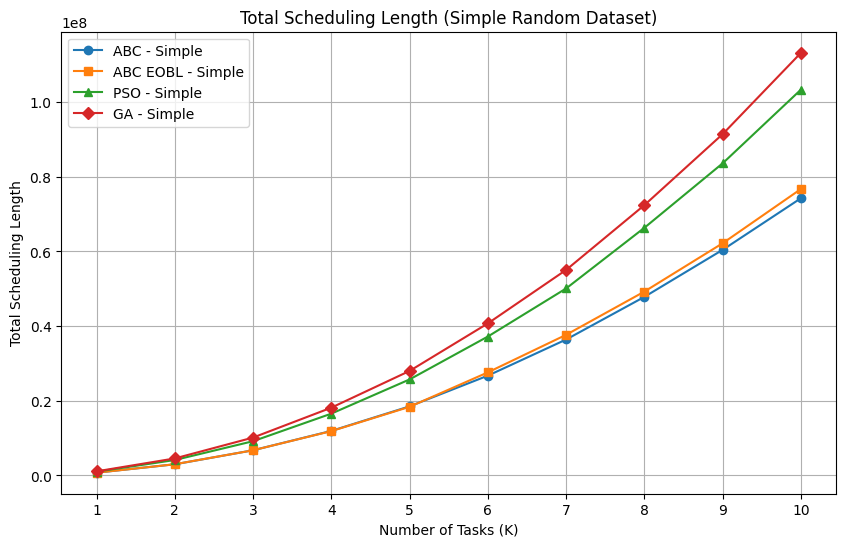
\includegraphics[width=0.75\linewidth]{gambar/Grafik Scheduling Length Simple Random.png}
    \caption{Grafik \textit{scheduling length simple random}}
\end{figure}

\begin{figure} [H]
    \centering
    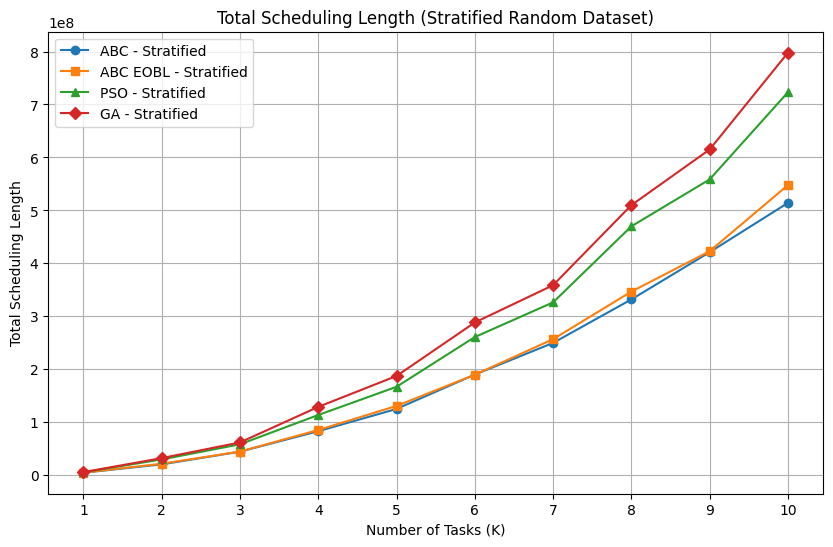
\includegraphics[width=0.75\linewidth]{gambar/Grafik Scheduling Length Stratified Random.png}
    \caption{Grafik \textit{scheduling length stratified random}}
\end{figure}

\newpage

\begin{figure} [H]
    \centering
    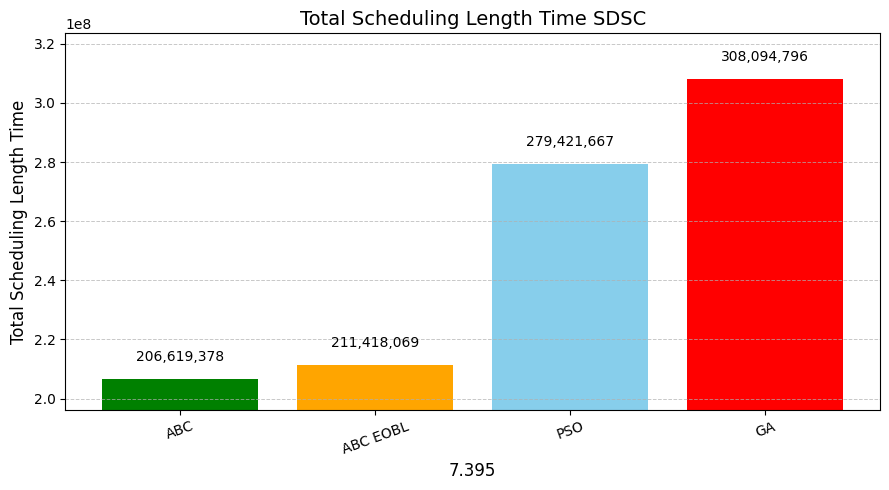
\includegraphics[width=0.75\linewidth]{gambar/Grafik Scheduling Length SDSC.png}
    \caption{Grafik \textit{scheduling length} SDSC}
\end{figure}

\begin{figure} [H]
    \centering
    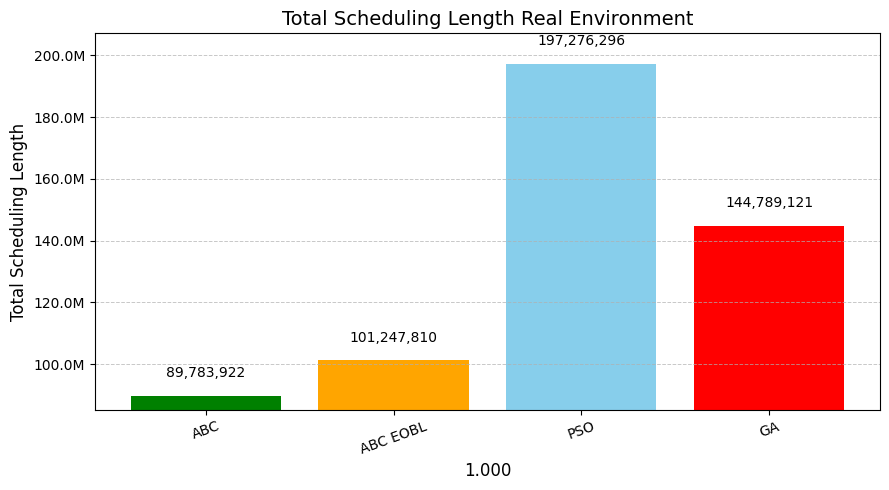
\includegraphics[width=0.75\linewidth]{gambar/Grafik Scheduling Length Real Environment.png}
    \caption{Grafik \textit{scheduling length real environment}}
\end{figure}

\subsection{\textit{Throughput} (\textit{Higher Better})}
\textit{Throughput} adalah jumlah tugas yang berhasil diselesaikan dalam satu unit waktu. Semakin tinggi nilai \textit{throughput}, semakin baik kinerja algoritma dalam menyelesaikan tugas secara efisien.

\newpage

\begin{table} [H]
\centering
\caption{\textit{Throughput simple random}}
\begin{tabular}{|>{\raggedleft\arraybackslash}m{0.12\linewidth}|
                >{\raggedleft\arraybackslash}m{0.17\linewidth}|
                >{\raggedleft\arraybackslash}m{0.17\linewidth}|
                >{\raggedleft\arraybackslash}m{0.17\linewidth}|
                >{\raggedleft\arraybackslash}m{0.17\linewidth}|}
\rowcolor{blue!30}
\hline
\multicolumn{1}{|>{\centering\arraybackslash}m{0.12\linewidth}|}{\textbf{\textit{Cloudlets}}} & 
\multicolumn{1}{>{\centering\arraybackslash}m{0.17\linewidth}|}{\textbf{ABC \textit{Simple}}} & 
\multicolumn{1}{>{\centering\arraybackslash}m{0.17\linewidth}|}{\textbf{ABC EOBL \textit{Simple}}} & 
\multicolumn{1}{>{\centering\arraybackslash}m{0.17\linewidth}|}{\textbf{PSO \textit{Simple}}} & 
\multicolumn{1}{>{\centering\arraybackslash}m{0.17\linewidth}|}{\textbf{GA \textit{Simple}}} \\
\hline
1.000 & 0,4164 & 0,4281 & 0,3060 & 0,3124 \\
\hline
2.000 & 0,4380 & 0,4249 & 0,3280 & 0,3272 \\
\hline
3.000 & 0,4603 & 0,4419 & 0,3370 & 0,3418 \\
\hline
4.000 & 0,4564 & 0,4698 & 0,3330 & 0,3426 \\
\hline
5.000 & 0,4753 & 0,4792 & 0,3430 & 0,3476 \\
\hline
6.000 & 0,4792 & 0,4435 & 0,3470 & 0,3483 \\
\hline
7.000 & 0,4803 & 0,4452 & 0,3540 & 0,3564 \\
\hline
8.000 & 0,4893 & 0,4548 & 0,3460 & 0,3587 \\
\hline
9.000 & 0,4920 & 0,4574 & 0,3500 & 0,3616 \\
\hline
10.000 & 0,4952 & 0,4547 & 0,3550 & 0,3601 \\
\hline
\textbf{AVG} & \textcolor{green}{0,4682} & 0,4500 & 0,3399 & 0,3457 \\
\hline
\end{tabular}
\end{table}

\begin{table} [H]
\centering
\caption{\textit{Throughput stratified random}}
\begin{tabular}{|>{\raggedleft\arraybackslash}m{0.12\linewidth}|
                >{\raggedleft\arraybackslash}m{0.17\linewidth}|
                >{\raggedleft\arraybackslash}m{0.17\linewidth}|
                >{\raggedleft\arraybackslash}m{0.17\linewidth}|
                >{\raggedleft\arraybackslash}m{0.17\linewidth}|}
\rowcolor{blue!30}
\hline
\multicolumn{1}{|>{\centering\arraybackslash}m{0.12\linewidth}|}{\textbf{\textit{Cloudlets}}} & 
\multicolumn{1}{>{\centering\arraybackslash}m{0.17\linewidth}|}{\textbf{ABC \textit{Stratified}}} & 
\multicolumn{1}{>{\centering\arraybackslash}m{0.17\linewidth}|}{\textbf{ABC EOBL \textit{Stratified}}} & 
\multicolumn{1}{>{\centering\arraybackslash}m{0.17\linewidth}|}{\textbf{PSO \textit{Stratified}}} & 
\multicolumn{1}{>{\centering\arraybackslash}m{0.17\linewidth}|}{\textbf{GA \textit{Stratified}}} \\
\hline
1.000 & 0,0282 & 0,0286 & 0,0336 & 0,0296 \\
\hline
2.000 & 0,0380 & 0,0379 & 0,0289 & 0,0271 \\
\hline
3.000 & 0,0466 & 0,0449 & 0,0421 & 0,0418 \\
\hline
4.000 & 0,0486 & 0,0442 & 0,0363 & 0,0361 \\
\hline
5.000 & 0,0518 & 0,0543 & 0,0423 & 0,0381 \\
\hline
6.000 & 0,0500 & 0,0517 & 0,0403 & 0,0369 \\
\hline
7.000 & 0,0575 & 0,0534 & 0,0450 & 0,0418 \\
\hline
8.000 & 0,0552 & 0,0544 & 0,0404 & 0,0395 \\
\hline
9.000 & 0,0570 & 0,0577 & 0,0435 & 0,0431 \\
\hline
10.000 & 0,0588 & 0,0523 & 0,0415 & 0,0426 \\
\hline
\textbf{AVG} & \textcolor{green}{0,0492} & 0,0479 & 0,0394 & 0,0377 \\
\hline
\end{tabular}
\end{table}

\begin{table} [H]
\centering
\caption{\textit{Throughput} SDSC}
\begin{tabular}{|>{\raggedleft\arraybackslash}m{0.12\linewidth}|
                >{\raggedleft\arraybackslash}m{0.15\linewidth}|
                >{\raggedleft\arraybackslash}m{0.25\linewidth}|
                >{\raggedleft\arraybackslash}m{0.15\linewidth}|
                >{\raggedleft\arraybackslash}m{0.15\linewidth}|}
\rowcolor{blue!30}
\hline
\multicolumn{1}{|>{\centering\arraybackslash}m{0.12\linewidth}|}{\textbf{\textit{Cloudlets}}} & 
\multicolumn{1}{>{\centering\arraybackslash}m{0.15\linewidth}|}{\textbf{ABC SDSC}} & 
\multicolumn{1}{>{\centering\arraybackslash}m{0.25\linewidth}|}{\textbf{ABC EOBL SDSC}} & 
\multicolumn{1}{>{\centering\arraybackslash}m{0.15\linewidth}|}{\textbf{PSO SDSC}} & 
\multicolumn{1}{>{\centering\arraybackslash}m{0.15\linewidth}|}{\textbf{GA SDSC}} \\
\hline
7.395 & \textcolor{green}{0,0674} & 0,0666 & 0,0526 & 0,0534 \\
\hline
\end{tabular}
\end{table}

\begin{table} [H]
\centering
\caption{\textit{Throughput real environment}}
\begin{tabular}{|>{\raggedleft\arraybackslash}m{0.1\linewidth}|
                >{\raggedleft\arraybackslash}m{0.17\linewidth}|
                >{\raggedleft\arraybackslash}m{0.17\linewidth}|
                >{\raggedleft\arraybackslash}m{0.17\linewidth}|
                >{\raggedleft\arraybackslash}m{0.17\linewidth}|}
\rowcolor{blue!30}
\hline
\multicolumn{1}{|>{\centering\arraybackslash}m{0.1\linewidth}|}{\textbf{\textit{Task}}} & 
\multicolumn{1}{>{\centering\arraybackslash}m{0.17\linewidth}|}{\textbf{ABC RE}} & 
\multicolumn{1}{>{\centering\arraybackslash}m{0.17\linewidth}|}{\textbf{ABC EOBL RE}} & 
\multicolumn{1}{>{\centering\arraybackslash}m{0.17\linewidth}|}{\textbf{PSO RE}} & 
\multicolumn{1}{>{\centering\arraybackslash}m{0.17\linewidth}|}{\textbf{GA RE}} \\
\hline
1.000 & \textcolor{green}{5,55} & 5,31 & 2,90 & 3,49 \\
\hline
\end{tabular}
\end{table}

Berdasarkan hasil pengujian yang disajikan pada tabel dan grafik, algoritma \textit{Artificial Bee Colony} (ABC) secara konsisten menunjukkan nilai \textit{throughput} tertinggi pada seluruh \textit{dataset} yang diuji, baik pada \textit{simple random}, \textit{stratified random}, maupun SDSC. Hal ini mengindikasikan bahwa ABC memiliki kapasitas penyelesaian tugas per satuan waktu yang paling optimal dibandingkan dengan algoritma lainnya.

Algoritma ABC dengan \textit{Elite Opposition-Based Learning} (EOBL) menempati posisi kedua, dengan nilai \textit{throughput} yang sedikit lebih rendah dibandingkan ABC, tetapi masih lebih tinggi daripada algoritma \textit{Particle Swarm Optimization} (PSO) dan \textit{Genetic Algorithm} (GA).

Keunggulan \textit{throughput} ABC ini disebabkan oleh mekanisme pencarian solusi yang efisien dan distribusi tugas yang optimal, memungkinkan penyelesaian lebih banyak tugas dalam waktu yang lebih singkat. Meskipun ABC-EOBL dirancang untuk memperbaiki pencarian solusi dengan menghindari jebakan lokal dan meningkatkan eksplorasi, proses ini mengarah pada evaluasi solusi lawan yang lebih banyak, yang berpotensi mengurangi efisiensi pencarian dan alokasi tugas dalam waktu singkat. Dengan kata lain, meskipun ABC-EOBL dapat memperbaiki kualitas solusi dengan memperluas ruang pencarian, proses pencarian yang lebih kompleks ini mengurangi kemampuan algoritma untuk menyelesaikan lebih banyak tugas dalam satuan waktu yang terbatas, sehingga menyebabkan penurunan nilai \textit{throughput} jika dibandingkan dengan ABC yang lebih efisien dalam distribusi tugas dan konvergensi solusi.

\begin{figure} [H]
    \centering
    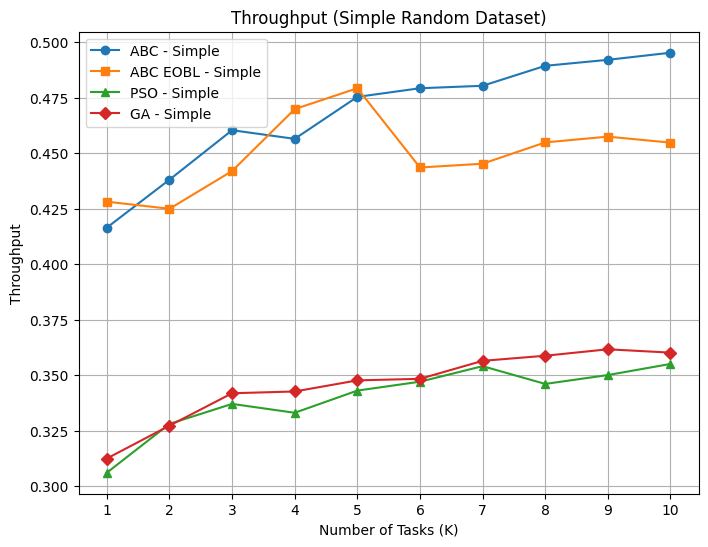
\includegraphics[width=0.75\linewidth]{gambar/Grafik Throughput Simple Random.png}
    \caption{Grafik \textit{throughput simple random}}
\end{figure}

\newpage

\begin{figure} [H]
    \centering
    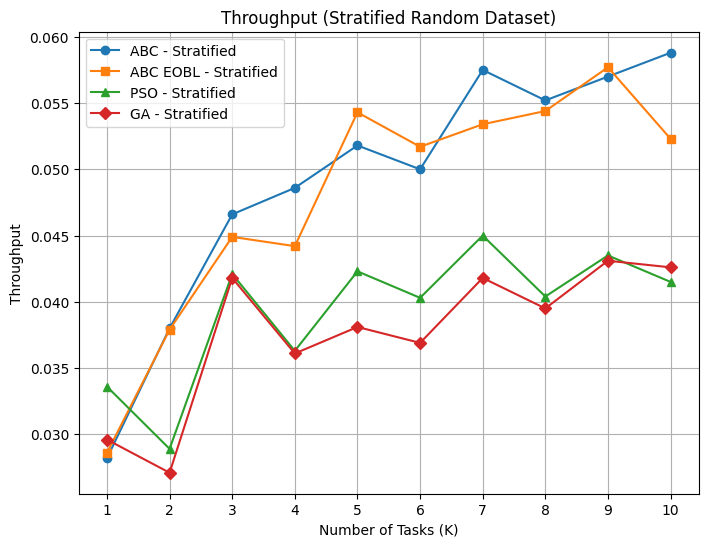
\includegraphics[width=0.75\linewidth]{gambar/Grafik Throughput Stratified Random.png}
    \caption{Grafik \textit{throughput stratified random}}
\end{figure}

\begin{figure} [H]
    \centering
    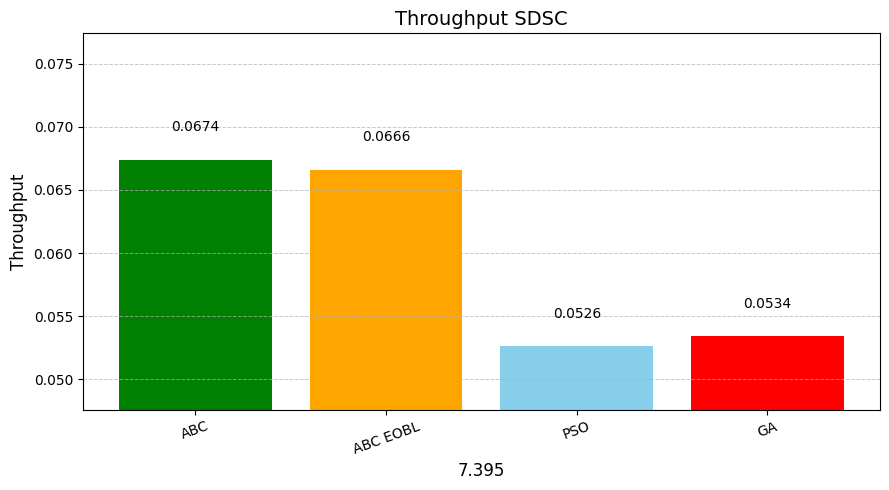
\includegraphics[width=0.75\linewidth]{gambar/Grafik Throughput SDSC.png}
    \caption{Grafik \textit{throughput} SDSC}
\end{figure}

\newpage

\begin{figure} [H]
    \centering
    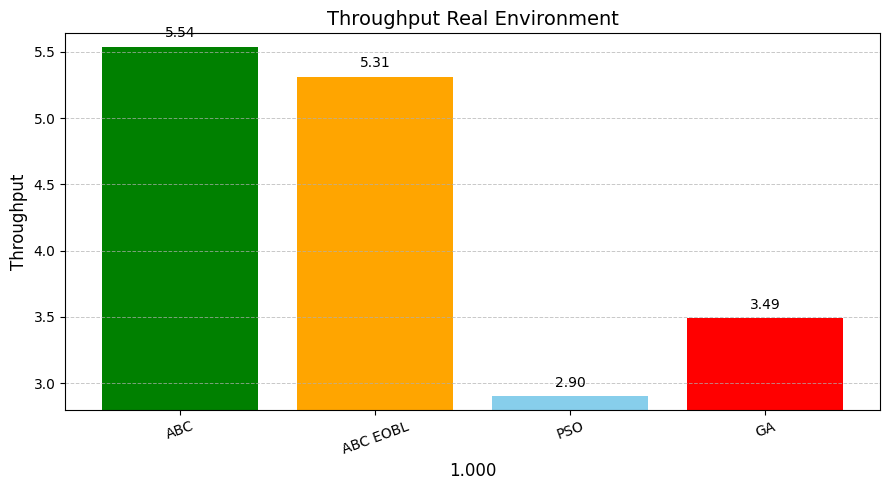
\includegraphics[width=0.75\linewidth]{gambar/Grafik Throughput Real Environment.png}
    \caption{Grafik \textit{throughput real environment}}
\end{figure}

\subsection{\textit{Resource Utilization} (\textit{Higher Better})}
\textit{Resource utilization} mengukur seberapa optimal sumber daya \textit{cloud} digunakan oleh algoritma dalam penjadwalan tugas. Semakin tinggi nilai \textit{resource utilization}, semakin efisien algoritma dalam memanfaatkan sumber daya yang tersedia.

\begin{table} [H]
\centering
\caption{\textit{Resource utilization simple random}}
\begin{tabular}{|>{\raggedleft\arraybackslash}m{0.12\linewidth}|
                >{\raggedleft\arraybackslash}m{0.17\linewidth}|
                >{\raggedleft\arraybackslash}m{0.17\linewidth}|
                >{\raggedleft\arraybackslash}m{0.17\linewidth}|
                >{\raggedleft\arraybackslash}m{0.17\linewidth}|}
\rowcolor{blue!30}
\hline
\multicolumn{1}{|>{\centering\arraybackslash}m{0.12\linewidth}|}{\textbf{\textit{Cloudlets}}} & 
\multicolumn{1}{>{\centering\arraybackslash}m{0.17\linewidth}|}{\textbf{ABC \textit{Simple}}} & 
\multicolumn{1}{>{\centering\arraybackslash}m{0.17\linewidth}|}{\textbf{ABC EOBL \textit{Simple}}} & 
\multicolumn{1}{>{\centering\arraybackslash}m{0.17\linewidth}|}{\textbf{PSO \textit{Simple}}} & 
\multicolumn{1}{>{\centering\arraybackslash}m{0.17\linewidth}|}{\textbf{GA \textit{Simple}}} \\
\hline
1.000 & 46,19 & 47,69 & 32,58 & 32,76 \\
\hline
2.000 & 48,42 & 47,05 & 34,73 & 34,05 \\
\hline
3.000 & 51,14 & 49,10 & 35,76 & 35,76 \\
\hline
4.000 & 50,39 & 51,98 & 35,14 & 35,58 \\
\hline
5.000 & 52,50 & 52,99 & 36,20 & 36,13 \\
\hline
6.000 & 52,99 & 48,83 & 36,61 & 36,20 \\
\hline
7.000 & 53,17 & 49,06 & 37,45 & 37,13 \\
\hline
8.000 & 54,20 & 50,19 & 36,63 & 37,39 \\
\hline
9.000 & 54,50 & 50,50 & 37,00 & 37,69 \\
\hline
10.000 & 54,82 & 50,09 & 37,45 & 37,46 \\
\hline
\textbf{AVG} & \textcolor{green}{51,83} & 49,75 & 35,96 & 36,02 \\
\hline
\end{tabular}
\end{table}

\newpage

\begin{table} [H]
\centering
\caption{\textit{Resource utilization stratified random}}
\begin{tabular}{|>{\raggedleft\arraybackslash}m{0.12\linewidth}|
                >{\raggedleft\arraybackslash}m{0.17\linewidth}|
                >{\raggedleft\arraybackslash}m{0.17\linewidth}|
                >{\raggedleft\arraybackslash}m{0.17\linewidth}|
                >{\raggedleft\arraybackslash}m{0.17\linewidth}|}
\rowcolor{blue!30}
\hline
\multicolumn{1}{|>{\centering\arraybackslash}m{0.12\linewidth}|}{\textbf{\textit{Cloudlets}}} & 
\multicolumn{1}{>{\centering\arraybackslash}m{0.17\linewidth}|}{\textbf{ABC \textit{Stratified}}} & 
\multicolumn{1}{>{\centering\arraybackslash}m{0.17\linewidth}|}{\textbf{ABC EOBL \textit{Stratified}}} & 
\multicolumn{1}{>{\centering\arraybackslash}m{0.17\linewidth}|}{\textbf{PSO \textit{Stratified}}} & 
\multicolumn{1}{>{\centering\arraybackslash}m{0.17\linewidth}|}{\textbf{GA \textit{Stratified}}} \\
\hline
1.000 & 25,51 & 25,32 & 29,23 & 25,84 \\
\hline
2.000 & 32,64 & 32,12 & 23,36 & 21,60 \\
\hline
3.000 & 40,93 & 39,73 & 35,71 & 34,94 \\
\hline
4.000 & 41,69 & 37,76 & 29,48 & 28,77 \\
\hline
5.000 & 45,15 & 47,15 & 35,42 & 31,18 \\
\hline
6.000 & 42,85 & 44,19 & 32,76 & 29,36 \\
\hline
7.000 & 49,82 & 46,13 & 37,36 & 34,04 \\
\hline
8.000 & 47,43 & 46,69 & 32,92 & 31,55 \\
\hline
9.000 & 49,16 & 49,94 & 35,97 & 34,98 \\
\hline
10.000 & 50,40 & 44,47 & 33,68 & 33,91 \\
\hline
\textbf{AVG} & \textcolor{green}{42,56} & 41,35 & 32,59 & 30,62 \\
\hline
\end{tabular}
\end{table}

\begin{table} [H]
\centering
\caption{\textit{Resource utilization} SDSC}
\begin{tabular}{|>{\raggedleft\arraybackslash}m{0.12\linewidth}|
                >{\raggedleft\arraybackslash}m{0.15\linewidth}|
                >{\raggedleft\arraybackslash}m{0.25\linewidth}|
                >{\raggedleft\arraybackslash}m{0.15\linewidth}|
                >{\raggedleft\arraybackslash}m{0.15\linewidth}|}
\rowcolor{blue!30}
\hline
\multicolumn{1}{|>{\centering\arraybackslash}m{0.12\linewidth}|}{\textbf{\textit{Cloudlets}}} & 
\multicolumn{1}{>{\centering\arraybackslash}m{0.15\linewidth}|}{\textbf{ABC SDSC}} & 
\multicolumn{1}{>{\centering\arraybackslash}m{0.25\linewidth}|}{\textbf{ABC EOBL SDSC}} & 
\multicolumn{1}{>{\centering\arraybackslash}m{0.15\linewidth}|}{\textbf{PSO SDSC}} & 
\multicolumn{1}{>{\centering\arraybackslash}m{0.15\linewidth}|}{\textbf{GA SDSC}} \\
\hline
7.395 & \textcolor{green}{43,94} & 43,27 & 32,69 & 32,19 \\
\hline
\end{tabular}
\end{table}

\begin{table} [H]
\centering
\caption{\textit{Resource utilization real environment}}
\begin{tabular}{|>{\raggedleft\arraybackslash}m{0.1\linewidth}|
                >{\raggedleft\arraybackslash}m{0.17\linewidth}|
                >{\raggedleft\arraybackslash}m{0.17\linewidth}|
                >{\raggedleft\arraybackslash}m{0.17\linewidth}|
                >{\raggedleft\arraybackslash}m{0.17\linewidth}|}
\rowcolor{blue!30}
\hline
\multicolumn{1}{|>{\centering\arraybackslash}m{0.1\linewidth}|}{\textbf{\textit{Task}}} & 
\multicolumn{1}{>{\centering\arraybackslash}m{0.17\linewidth}|}{\textbf{ABC RE}} & 
\multicolumn{1}{>{\centering\arraybackslash}m{0.17\linewidth}|}{\textbf{ABC EOBL RE}} & 
\multicolumn{1}{>{\centering\arraybackslash}m{0.17\linewidth}|}{\textbf{PSO RE}} & 
\multicolumn{1}{>{\centering\arraybackslash}m{0.17\linewidth}|}{\textbf{GA RE}} \\
\hline
1.000 & \textcolor{green}{16,97} & 16,59 & 15,94 & 15,31 \\
\hline
\end{tabular}
\end{table}

Berdasarkan hasil pengujian yang disajikan pada tabel dan grafik, algoritma \textit{Artificial Bee Colony} (ABC) menunjukkan pemanfaatan sumber daya tertinggi pada seluruh \textit{dataset} yang diuji, baik pada \textit{simple random}, \textit{stratified random}, maupun SDSC. Hal ini menunjukkan bahwa ABC mampu mengalokasikan sumber daya secara lebih optimal dibandingkan dengan algoritma lainnya.

Algoritma ABC dengan \textit{Elite Opposition-Based Learning} (EOBL) menempati posisi kedua, dengan pemanfaatan yang sedikit lebih rendah dibandingkan ABC, namun masih lebih tinggi daripada \textit{Particle Swarm Optimization} (PSO) dan \textit{Genetic Algorithm} (GA).

Penurunan pemanfaatan sumber daya pada ABC-EOBL disebabkan oleh kompleksitas tambahan dari mekanisme EOBL, yang melibatkan evaluasi solusi lawan yang lebih banyak. Meskipun EOBL bertujuan untuk memperbaiki pencarian solusi dan menghindari jebakan lokal, proses ini membutuhkan lebih banyak waktu komputasi untuk memproses dan mengevaluasi solusi yang lebih banyak. Dengan meningkatnya jumlah solusi yang harus dievaluasi, waktu komputasi yang dibutuhkan menjadi lebih lama, sehingga menyebabkan alokasi sumber daya yang lebih banyak terbuang pada proses evaluasi dan seleksi, bukan pada penyelesaian tugas yang efektif. Akibatnya, alokasi sumber daya menjadi kurang optimal dibandingkan dengan algoritma ABC yang lebih sederhana dan efisien dalam distribusi tugas.

\newpage

\begin{figure} [H]
    \centering
    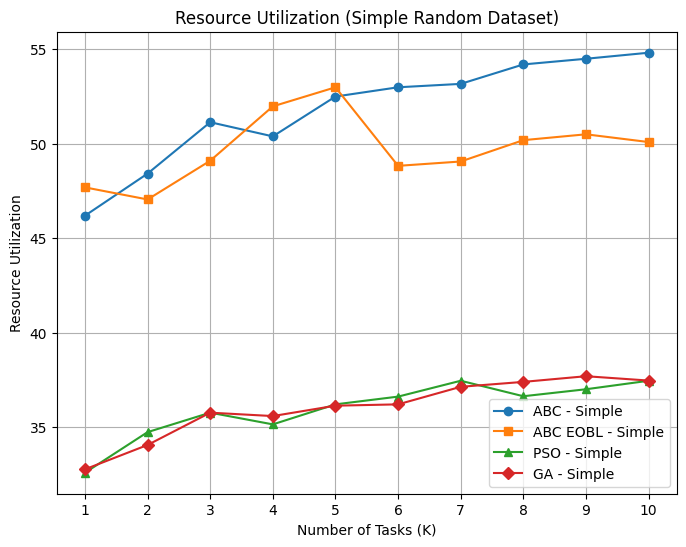
\includegraphics[width=0.75\linewidth]{gambar/Grafik Resource Utilization Simple Random.png}
    \caption{Grafik \textit{resource utilization simple random}}
\end{figure}

\begin{figure} [H]
    \centering
    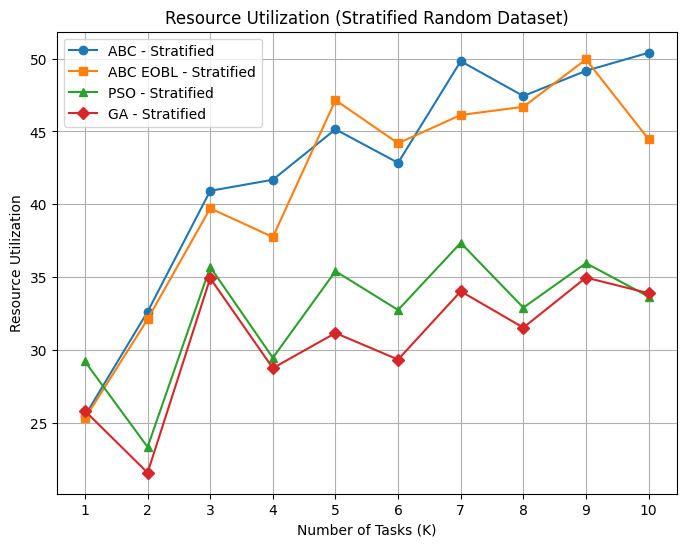
\includegraphics[width=0.75\linewidth]{gambar/Grafik Resource Utilization Stratified Random.png}
    \caption{Grafik \textit{resource utilization stratified random}}
\end{figure}

\newpage

\begin{figure} [H]
    \centering
    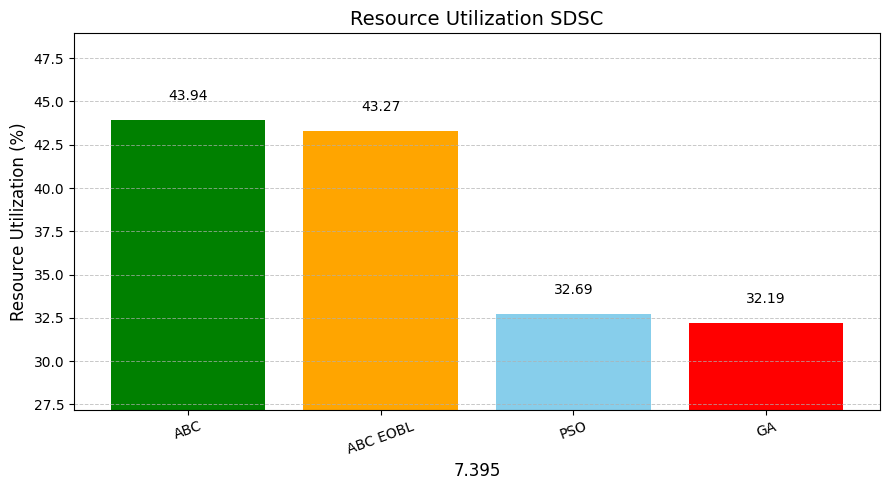
\includegraphics[width=0.75\linewidth]{gambar/Grafik Resource Utilization SDSC.png}
    \caption{Grafik \textit{resource utilization} SDSC}
\end{figure}

\begin{figure} [H]
    \centering
    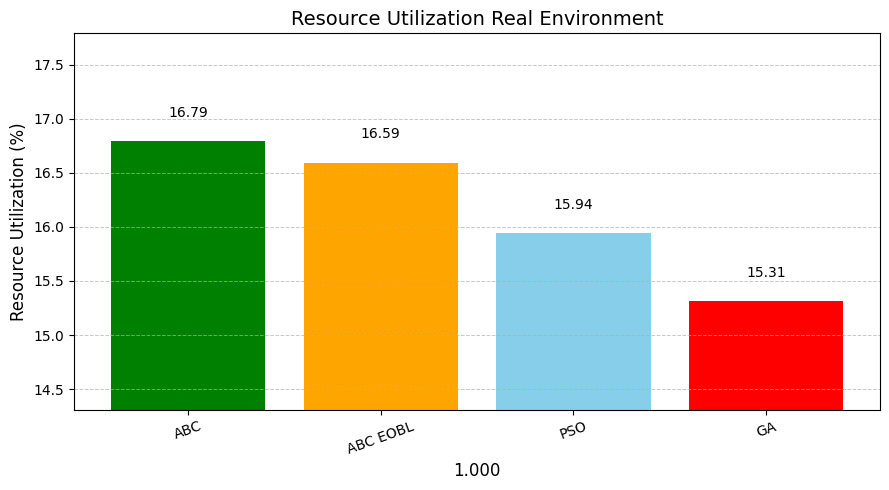
\includegraphics[width=0.75\linewidth]{gambar/Grafik Resource Utilization Real Environment.png}
    \caption{Grafik \textit{resource utilization real environment}}
\end{figure}

\subsection{\textit{Total Energy Consumption} (\textit{Lower Better})}
\textit{Total energy consumption} mengukur tingkat penggunaan energi yang dibutuhkan oleh semua sumber daya \textit{cloud}. Semakin rendah nilai dari parameter ini, semakin efisien algoritma dalam memanfaatkan energi, yang menunjukkan kinerja yang lebih baik.

\newpage

\begin{table} [H]
\centering
\caption{\textit{Total energy consumption simple random}}
\begin{tabular}{|>{\raggedleft\arraybackslash}m{0.12\linewidth}|
                >{\raggedleft\arraybackslash}m{0.17\linewidth}|
                >{\raggedleft\arraybackslash}m{0.17\linewidth}|
                >{\raggedleft\arraybackslash}m{0.17\linewidth}|
                >{\raggedleft\arraybackslash}m{0.17\linewidth}|}
\rowcolor{blue!30}
\hline
\multicolumn{1}{|>{\centering\arraybackslash}m{0.12\linewidth}|}{\textbf{\textit{Cloudlets}}} & 
\multicolumn{1}{>{\centering\arraybackslash}m{0.17\linewidth}|}{\textbf{ABC \textit{Simple}}} & 
\multicolumn{1}{>{\centering\arraybackslash}m{0.17\linewidth}|}{\textbf{ABC EOBL \textit{Simple}}} & 
\multicolumn{1}{>{\centering\arraybackslash}m{0.17\linewidth}|}{\textbf{PSO \textit{Simple}}} & 
\multicolumn{1}{>{\centering\arraybackslash}m{0.17\linewidth}|}{\textbf{GA \textit{Simple}}} \\
\hline
1.000 & 12,52 & 11,48 & 15,33 & 15,73 \\
\hline
2.000 & 20,45 & 23,04 & 30,07 & 30,88 \\
\hline
3.000 & 27,87 & 33,64 & 43,81 & 45,20 \\
\hline
4.000 & 38,33 & 43,61 & 59,17 & 60,46 \\
\hline
5.000 & 42,13 & 53,47 & 73,21 & 73,89 \\
\hline
6.000 & 53,22 & 68,83 & 88,15 & 89,40 \\
\hline
7.000 & 59,62 & 80,70 & 101,62 & 102,90 \\
\hline
8.000 & 68,75 & 91,68 & 118,04 & 117,50 \\
\hline
9.000 & 73,15 & 102,68 & 132,60 & 131,59 \\
\hline
10.000 & 90,62 & 114,18 & 145,75 & 146,19 \\
\hline
\textbf{AVG} & \textcolor{green}{48,67} & 62,33 & 80,78 & 81,37 \\
\hline
\end{tabular}
\end{table}

\begin{table} [H]
\centering
\caption{\textit{Total energy consumption stratified random}}
\begin{tabular}{|>{\raggedleft\arraybackslash}m{0.12\linewidth}|
                >{\raggedleft\arraybackslash}m{0.17\linewidth}|
                >{\raggedleft\arraybackslash}m{0.17\linewidth}|
                >{\raggedleft\arraybackslash}m{0.17\linewidth}|
                >{\raggedleft\arraybackslash}m{0.17\linewidth}|}
\rowcolor{blue!30}
\hline
\multicolumn{1}{|>{\centering\arraybackslash}m{0.12\linewidth}|}{\textbf{\textit{Cloudlets}}} & 
\multicolumn{1}{>{\centering\arraybackslash}m{0.17\linewidth}|}{\textbf{ABC \textit{Stratified}}} & 
\multicolumn{1}{>{\centering\arraybackslash}m{0.17\linewidth}|}{\textbf{ABC EOBL \textit{Stratified}}} & 
\multicolumn{1}{>{\centering\arraybackslash}m{0.17\linewidth}|}{\textbf{PSO \textit{Stratified}}} & 
\multicolumn{1}{>{\centering\arraybackslash}m{0.17\linewidth}|}{\textbf{GA \textit{Stratified}}} \\
\hline
1.000 & 130,93 & 125,19 & 125,80 & 122,14 \\
\hline
2.000 & 195,26 & 204,49 & 260,78 & 269,33 \\
\hline
3.000 & 279,38 & 278,69 & 315,51 & 315,64 \\
\hline
4.000 & 362,91 & 383,29 & 479,57 & 479,46 \\
\hline
5.000 & 420,67 & 421,32 & 535,27 & 560,04 \\
\hline
6.000 & 527,21 & 532,18 & 696,44 & 722,26 \\
\hline
7.000 & 563,93 & 596,23 & 711,64 & 758,35 \\
\hline
8.000 & 675,69 & 687,52 & 907,06 & 949,97 \\
\hline
9.000 & 739,10 & 731,50 & 952,50 & 993,14 \\
\hline
10.000 & 809,38 & 906,22 & 1.108,87 & 1.143,16 \\
\hline
\textbf{AVG} & \textcolor{green}{470,45} & 486,66 & 609,34 & 631,35 \\
\hline
\end{tabular}
\end{table}

\begin{table} [H]
\centering
\caption{\textit{Total energy consumption} SDSC}
\begin{tabular}{|>{\raggedleft\arraybackslash}m{0.12\linewidth}|
                >{\raggedleft\arraybackslash}m{0.15\linewidth}|
                >{\raggedleft\arraybackslash}m{0.25\linewidth}|
                >{\raggedleft\arraybackslash}m{0.15\linewidth}|
                >{\raggedleft\arraybackslash}m{0.15\linewidth}|}
\rowcolor{blue!30}
\hline
\multicolumn{1}{|>{\centering\arraybackslash}m{0.12\linewidth}|}{\textbf{\textit{Cloudlets}}} & 
\multicolumn{1}{>{\centering\arraybackslash}m{0.15\linewidth}|}{\textbf{ABC SDSC}} & 
\multicolumn{1}{>{\centering\arraybackslash}m{0.25\linewidth}|}{\textbf{ABC EOBL SDSC}} & 
\multicolumn{1}{>{\centering\arraybackslash}m{0.15\linewidth}|}{\textbf{PSO SDSC}} & 
\multicolumn{1}{>{\centering\arraybackslash}m{0.15\linewidth}|}{\textbf{GA SDSC}} \\
\hline
7.395 & \textcolor{green}{497,37} & 498,76 & 613,34 & 656,95 \\
\hline
\end{tabular}
\end{table}

Berdasarkan hasil pengujian yang disajikan pada tabel dan grafik, algoritma ABC menunjukkan konsumsi energi paling rendah pada seluruh \textit{dataset} yang diuji, baik pada \textit{simple random}, \textit{stratified random}, maupun SDSC. Ini menunjukkan bahwa ABC sangat efisien dalam memanfaatkan energi dibandingkan dengan algoritma lainnya.

Algoritma ABC dengan \textit{Elite Opposition-Based Learning} (EOBL) menempati posisi kedua, dengan konsumsi energi yang sedikit lebih tinggi dibandingkan ABC, namun tetap lebih baik dibandingkan dengan \textit{Particle Swarm Optimization} (PSO) dan \textit{Genetic Algorithm} (GA). Pada \textit{dataset} SDSC, selisih konsumsi energi antara ABC dan ABC-EOBL sangat kecil, yang menunjukkan bahwa meskipun penambahan strategi EOBL pada ABC memberikan sedikit peningkatan dalam efisiensi, ABC tetap menjadi pilihan terbaik dalam hal penghematan energi.

Peningkatan konsumsi energi pada algoritma ABC-EOBL disebabkan oleh tambahan kompleksitas dari proses evaluasi solusi lawan yang dilakukan oleh metode EOBL. Setiap evaluasi solusi lawan memerlukan lebih banyak perhitungan dan proses komputasi, yang berimbas pada penggunaan daya yang lebih tinggi. Meskipun EOBL bertujuan untuk memperbaiki pencarian solusi dan menghindari jebakan lokal, kompleksitas tambahan ini menyebabkan peningkatan waktu komputasi dan konsumsi energi yang lebih besar dibandingkan dengan algoritma ABC yang lebih sederhana dan langsung dalam alokasi tugas.

\begin{figure} [H]
    \centering
    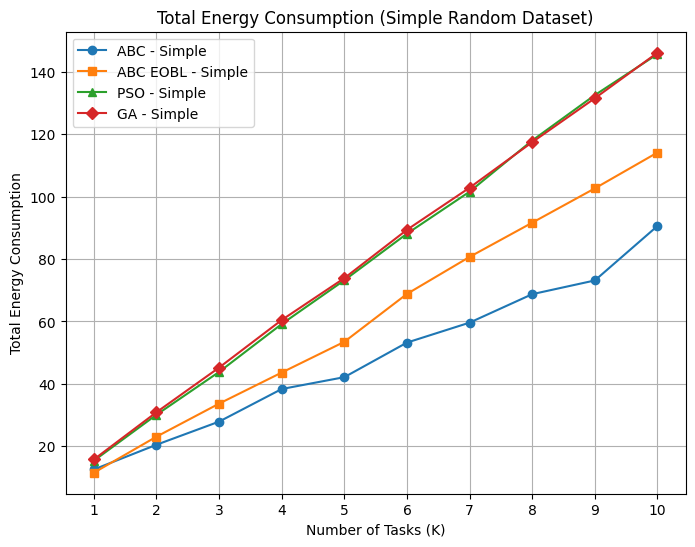
\includegraphics[width=0.75\linewidth]{gambar/Grafik Total Energy Consumption Simple Random.png}
    \caption{Grafik \textit{total energy consumption simple random}}
\end{figure}

\newpage

\begin{figure} [H]
    \centering
    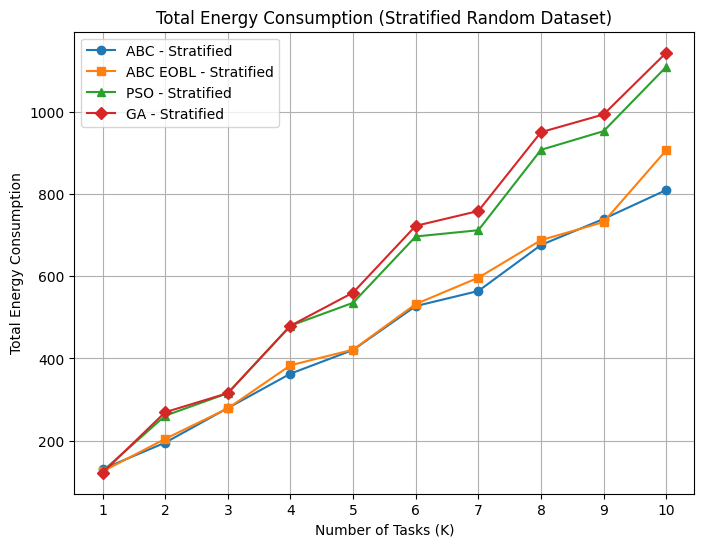
\includegraphics[width=0.75\linewidth]{gambar/Grafik Total Energy Consumption Stratified Random.png}
    \caption{Grafik \textit{total energy consumption stratified random}}
\end{figure}

\begin{figure} [H]
    \centering
    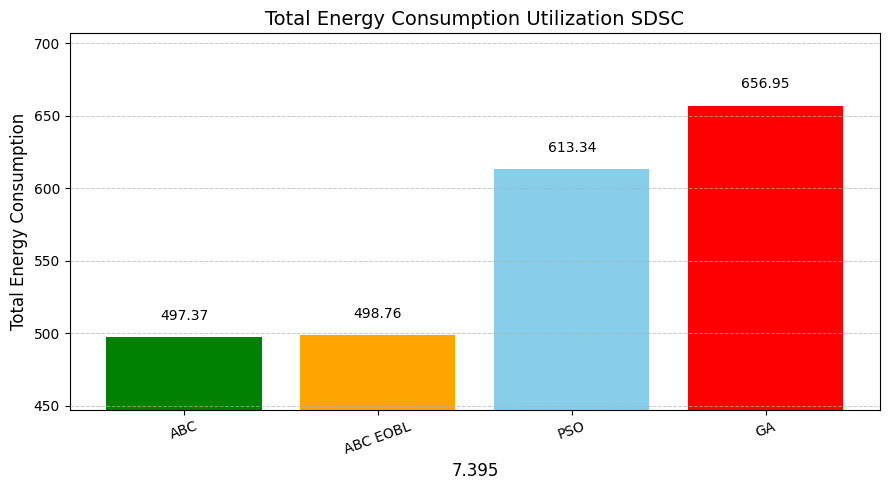
\includegraphics[width=0.75\linewidth]{gambar/Grafik Total Energy Consumption SDSC.png}
    \caption{Grafik \textit{total energy consumption} SDSC}
\end{figure}

\subsection{\textit{Imbalance Degree} (\textit{Lower Better})}
\textit{Imbalance degree} mengukur ketidakseimbangan dalam durasi pemrosesan tugas. Semakin rendah nilai \textit{imbalance degree}, semakin baik kinerja algoritma dalam mendistribusikan beban tugas secara merata, yang berarti durasi pemrosesan antar tugas lebih seimbang.

\newpage

\begin{table} [H]
\centering
\caption{\textit{Imbalance degree simple random}}
\begin{tabular}{|>{\raggedleft\arraybackslash}m{0.12\linewidth}|
                >{\raggedleft\arraybackslash}m{0.17\linewidth}|
                >{\raggedleft\arraybackslash}m{0.17\linewidth}|
                >{\raggedleft\arraybackslash}m{0.17\linewidth}|
                >{\raggedleft\arraybackslash}m{0.17\linewidth}|}
\rowcolor{blue!30}
\hline
\multicolumn{1}{|>{\centering\arraybackslash}m{0.12\linewidth}|}{\textbf{\textit{Cloudlets}}} & 
\multicolumn{1}{>{\centering\arraybackslash}m{0.17\linewidth}|}{\textbf{ABC \textit{Simple}}} & 
\multicolumn{1}{>{\centering\arraybackslash}m{0.17\linewidth}|}{\textbf{ABC EOBL \textit{Simple}}} & 
\multicolumn{1}{>{\centering\arraybackslash}m{0.17\linewidth}|}{\textbf{PSO \textit{Simple}}} & 
\multicolumn{1}{>{\centering\arraybackslash}m{0.17\linewidth}|}{\textbf{GA \textit{Simple}}} \\
\hline
1.000 & 1,80 & 1,80 & 1,88 & 1,89 \\
\hline
2.000 & 1,81 & 1,80 & 1,89 & 1,86 \\
\hline
3.000 & 1,80 & 1,80 & 1,88 & 1,91 \\
\hline
4.000 & 1,81 & 1,80 & 1,90 & 1,91 \\
\hline
5.000 & 1,81 & 1,80 & 1,90 & 1,92 \\
\hline
6.000 & 1,81 & 1,81 & 1,90 & 1,92 \\
\hline
7.000 & 1,81 & 1,81 & 1,89 & 1,92 \\
\hline
8.000 & 1,81 & 1,81 & 1,89 & 1,92 \\
\hline
9.000 & 1,81 & 1,81 & 1,89 & 1,92 \\
\hline
10.000 & 1,81 & 1,81 & 1,89 & 1,92 \\
\hline
\textbf{AVG} & 1,808 & \textcolor{green}{1,805} & 1,891 & 1,909 \\
\hline
\end{tabular}
\end{table}

\begin{table} [H]
\centering
\caption{\textit{Imbalance degree stratified random}}
\begin{tabular}{|>{\raggedleft\arraybackslash}m{0.12\linewidth}|
                >{\raggedleft\arraybackslash}m{0.17\linewidth}|
                >{\raggedleft\arraybackslash}m{0.17\linewidth}|
                >{\raggedleft\arraybackslash}m{0.17\linewidth}|
                >{\raggedleft\arraybackslash}m{0.17\linewidth}|}
\rowcolor{blue!30}
\hline
\multicolumn{1}{|>{\centering\arraybackslash}m{0.12\linewidth}|}{\textbf{\textit{Cloudlets}}} & 
\multicolumn{1}{>{\centering\arraybackslash}m{0.17\linewidth}|}{\textbf{ABC \textit{Stratified}}} & 
\multicolumn{1}{>{\centering\arraybackslash}m{0.17\linewidth}|}{\textbf{ABC EOBL \textit{Stratified}}} & 
\multicolumn{1}{>{\centering\arraybackslash}m{0.17\linewidth}|}{\textbf{PSO \textit{Stratified}}} & 
\multicolumn{1}{>{\centering\arraybackslash}m{0.17\linewidth}|}{\textbf{GA \textit{Stratified}}} \\
\hline
1.000 & 41,25 & 35,91 & 42,12 & 43,40 \\
\hline
2.000 & 44,90 & 42,23 & 49,72 & 48,72 \\
\hline
3.000 & 45,47 & 44,18 & 47,53 & 47,02 \\
\hline
4.000 & 46,14 & 43,13 & 48,75 & 49,94 \\
\hline
5.000 & 46,41 & 45,99 & 48,47 & 49,68 \\
\hline
6.000 & 47,01 & 46,90 & 48,80 & 50,67 \\
\hline
7.000 & 46,86 & 46,46 & 48,94 & 49,34 \\
\hline
8.000 & 47,23 & 47,03 & 49,77 & 50,78 \\
\hline
9.000 & 46,74 & 46,60 & 48,87 & 50,08 \\
\hline
10.000 & 47,43 & 47,01 & 50,08 & 51,01 \\
\hline
\textbf{AVG} & 45,94 & \textcolor{green}{44,54} & 48,31 & 49,06 \\
\hline
\end{tabular}
\end{table}

\begin{table} [H]
\centering
\caption{\textit{Imbalance degree} SDSC}
\begin{tabular}{|>{\raggedleft\arraybackslash}m{0.12\linewidth}|
                >{\raggedleft\arraybackslash}m{0.15\linewidth}|
                >{\raggedleft\arraybackslash}m{0.25\linewidth}|
                >{\raggedleft\arraybackslash}m{0.15\linewidth}|
                >{\raggedleft\arraybackslash}m{0.15\linewidth}|}
\rowcolor{blue!30}
\hline
\multicolumn{1}{|>{\centering\arraybackslash}m{0.12\linewidth}|}{\textbf{\textit{Cloudlets}}} & 
\multicolumn{1}{>{\centering\arraybackslash}m{0.15\linewidth}|}{\textbf{ABC SDSC}} & 
\multicolumn{1}{>{\centering\arraybackslash}m{0.25\linewidth}|}{\textbf{ABC EOBL SDSC}} & 
\multicolumn{1}{>{\centering\arraybackslash}m{0.15\linewidth}|}{\textbf{PSO SDSC}} & 
\multicolumn{1}{>{\centering\arraybackslash}m{0.15\linewidth}|}{\textbf{GA SDSC}} \\
\hline
7.395 & 56,01 & \textcolor{green}{54,78} & 56,88 & 56,83 \\
\hline
\end{tabular}
\end{table}

\begin{table} [H]
\centering
\caption{\textit{Imbalance degree real environment}}
\begin{tabular}{|>{\raggedleft\arraybackslash}m{0.1\linewidth}|
                >{\raggedleft\arraybackslash}m{0.17\linewidth}|
                >{\raggedleft\arraybackslash}m{0.17\linewidth}|
                >{\raggedleft\arraybackslash}m{0.17\linewidth}|
                >{\raggedleft\arraybackslash}m{0.17\linewidth}|}
\rowcolor{blue!30}
\hline
\multicolumn{1}{|>{\centering\arraybackslash}m{0.1\linewidth}|}{\textbf{\textit{Task}}} & 
\multicolumn{1}{>{\centering\arraybackslash}m{0.17\linewidth}|}{\textbf{ABC RE}} & 
\multicolumn{1}{>{\centering\arraybackslash}m{0.17\linewidth}|}{\textbf{ABC EOBL RE}} & 
\multicolumn{1}{>{\centering\arraybackslash}m{0.17\linewidth}|}{\textbf{PSO RE}} & 
\multicolumn{1}{>{\centering\arraybackslash}m{0.17\linewidth}|}{\textbf{GA RE}} \\
\hline
1.000 & 0,334 & \textcolor{green}{0,246} & 1,395 & 0,861 \\
\hline
\end{tabular}
\end{table}

\newpage

Berdasarkan hasil pengujian yang disajikan pada tabel dan grafik eksperimen, algoritma \textit{Artificial Bee Colony} (ABC) yang diintegrasikan dengan \textit{Elite Opposition-Based Learning} menunjukkan \textit{imbalance degree} terendah dibandingkan dengan ABC, PSO, dan GA. Hal ini menunjukkan bahwa integrasi EOBL memungkinkan distribusi tugas yang lebih merata dan seimbang, karena mekanisme EOBL membantu menghindari jebakan lokal dan memperluas eksplorasi solusi yang lebih optimal.

Pada \textit{dataset simple random} dan \textit{stratified random}, ABC-EOBL juga menunjukkan nilai \textit{imbalance degree} yang lebih rendah dibandingkan dengan algoritma lainnya. Ini menandakan bahwa algoritma ABC-EOBL lebih efektif dalam distribusi beban tugas, berkat kemampuan EOBL dalam menjaga keseimbangan durasi pemrosesan tugas. Pendekatan ini mencegah ketidakseimbangan beban kerja antar tugas, mengoptimalkan pemanfaatan sumber daya, dan meningkatkan efisiensi secara keseluruhan.

Secara keseluruhan, integrasi EOBL pada ABC meningkatkan kemampuan algoritma untuk mengeksplorasi solusi lebih luas, yang dimana menghasilkan distribusi beban tugas yang lebih seimbang dan menghasilkan \textit{imbalance degree} yang lebih rendah. Hal ini menjadikan ABC-EOBL lebih efektif dalam mengoptimalkan alokasi sumber daya dan meningkatkan keseimbangan dalam penyelesaian tugas.

\begin{figure} [H]
    \centering
    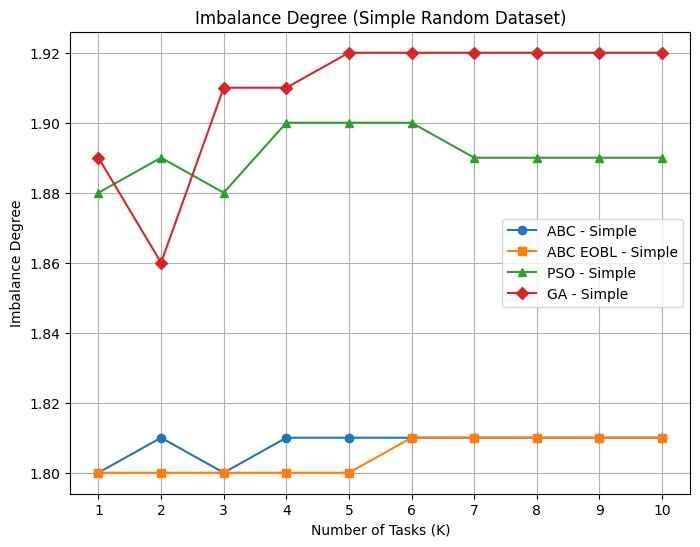
\includegraphics[width=0.75\linewidth]{gambar/Grafik Imbalance Degree Simple Random.png}
    \caption{Grafik \textit{imbalance degree simple random}}
\end{figure}

\newpage

\begin{figure} [H]
    \centering
    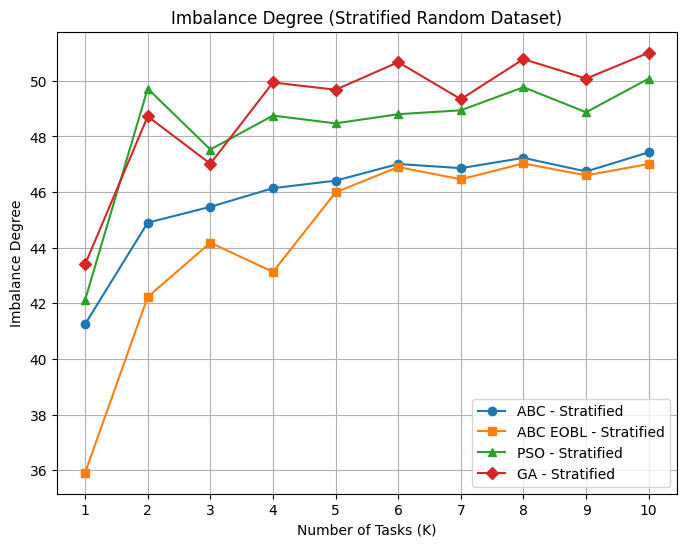
\includegraphics[width=0.75\linewidth]{gambar/Grafik Imbalance Degree Stratified Random.png}
    \caption{Grafik \textit{imbalance degree stratified random}}
\end{figure}

\begin{figure} [H]
    \centering
    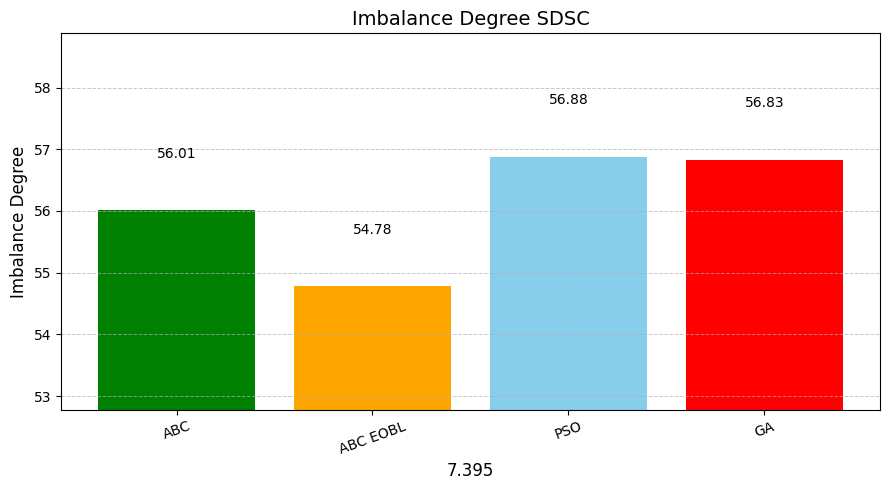
\includegraphics[width=0.75\linewidth]{gambar/Grafik Imbalance Degree SDSC.png}
    \caption{Grafik \textit{imbalance degree} SDSC}
\end{figure}

\newpage

\begin{figure} [H]
    \centering
    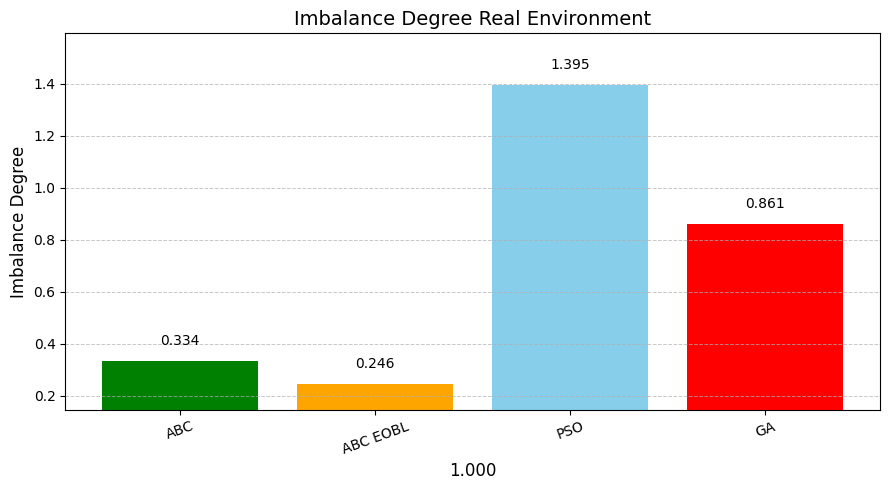
\includegraphics[width=0.75\linewidth]{gambar/Grafik Imbalance Degree Real Environment.png}
    \caption{Grafik \textit{imbalance degree real environment}}
\end{figure}

\subsection{Analisis Performa}
Analisis performa algoritma pada tiga \textit{dataset} yang berbeda, yaitu \textit{simple random}, \textit{stratified random}, dan SDSC menunjukkan perbedaan dalam kinerja masing-masing algoritma berdasarkan berbagai parameter evaluasi. Tabel \ref{tabel:Perbandingan Algoritma22} merangkum algoritma terbaik yang diidentifikasi berdasarkan performa terbaik pada setiap parameter.

\begin{table} [H]
\label{tabel:Perbandingan Algoritma22}
\centering
\caption{Perbandingan algoritma pada berbagai parameter di lingkungan nyata}
\begin{tabular}{|>{\raggedright\arraybackslash}m{0.15\linewidth}|
                >{\centering\arraybackslash}m{0.15\linewidth}|
                >{\centering\arraybackslash}m{0.2\linewidth}|
                >{\centering\arraybackslash}m{0.15\linewidth}|
                >{\centering\arraybackslash}m{0.15\linewidth}|}
\rowcolor{blue!30}
\hline
\multicolumn{1}{|>{\centering\arraybackslash}m{0.15\linewidth}|}{\textbf{Parameter}} & 
\multicolumn{1}{>{\centering\arraybackslash}m{0.15\linewidth}|}{\textbf{\textit{Simple Random}}} & 
\multicolumn{1}{>{\centering\arraybackslash}m{0.2\linewidth}|}{\textbf{\textit{Stratified Random}}} & 
\multicolumn{1}{>{\centering\arraybackslash}m{0.15\linewidth}|}{\textbf{SDSC}} &
\multicolumn{1}{>{\centering\arraybackslash}m{0.15\linewidth}|}{\textbf{\textit{Real Environment}}} \\
\hline
\textit{Makespan} & \cellcolor{green!30} ABC & \cellcolor{green!30} ABC & \cellcolor{green!30} ABC & \cellcolor{green!30} ABC \\
\hline
\textit{Average Start Time} & \cellcolor{green!30} ABC & \cellcolor{green!30} ABC & \cellcolor{green!30} ABC & \cellcolor{green!30} ABC \\
\hline
\textit{Average Finish Time} & \cellcolor{green!30} ABC & \cellcolor{green!30} ABC & \cellcolor{green!30} ABC & \cellcolor{green!30} ABC \\
\hline
\textit{Average Execution Time} & GA & GA & GA & \cellcolor{green!30} ABC \\
\hline
\textit{Average Waiting Time} & \cellcolor{green!30} ABC & \cellcolor{green!30} ABC & \cellcolor{green!30} ABC & \cellcolor{green!30} ABC \\
\hline
\textit{Scheduling Length} & \cellcolor{green!30} ABC & \cellcolor{green!30} ABC & \cellcolor{green!30} ABC & \cellcolor{green!30} ABC \\
\hline
\textit{Throughput} & \cellcolor{green!30} ABC & \cellcolor{green!30} ABC & \cellcolor{green!30} ABC & \cellcolor{green!30} ABC \\
\hline
\textit{Resource Utilization} & \cellcolor{green!30} ABC & \cellcolor{green!30} ABC & \cellcolor{green!30} ABC & \cellcolor{green!30} ABC \\
\hline
\textit{Total Energy Consumption} & \cellcolor{green!30} ABC & \cellcolor{green!30} ABC & \cellcolor{green!30} ABC & - \\
\hline
\textit{Imbalance Degree} & \cellcolor{green!30} ABC - EOBL & \cellcolor{green!30} ABC - EOBL & \cellcolor{green!30} ABC - EOBL & \cellcolor{green!30} ABC - EOBL \\
\hline
\end{tabular}
\end{table}

Pada \textit{dataset simple random}, ABC unggul dalam \textit{makespan} (\textit{lower better}) dengan nilai 11.480,73, yang lebih baik ($\approx 19,91\%$), \textit{average start time} (\textit{lower better}) dengan nilai 4.051,48, yang lebih baik ($\approx 22,13\%$), \textit{average finish time} (\textit{lower better}) dengan nilai 4.108,00, yang lebih baik ($\approx 21,95\%$), \textit{average waiting time} (\textit{lower better}) dengan nilai 2,13, yang lebih baik ($\approx 19,15\%$), \textit{scheduling length} (\textit{lower better}) dengan nilai 28.662.162,90, yang lebih baik ($\approx 21,51\%$), \textit{throughput} (\textit{higher better}) dengan nilai 0,4682, yang lebih baik ($\approx 16,54\%$), \textit{resource utilization} (\textit{higher better}) dengan nilai 51,83, yang lebih baik ($\approx 19,03\%$), \textit{total energy consumption} (\textit{lower better}) dengan nilai 48,67, yang lebih baik ($\approx 33,94\%$) dibandingkan ketiga algoritma lain. Namun, ABC EOBL menunjukkan keunggulan dalam hal \textit{imbalance degree} (\textit{lower better}), dengan nilai 1,808, yang lebih rendah ($\approx 3,39\%$).

Pada \textit{dataset stratified random}, ABC dominan dalam \textit{makespan} (\textit{lower better}) dengan nilai 105.823,95, yang lebih baik ($\approx 16,81\%$), \textit{average start time} (\textit{lower better}) dengan nilai 28.231,33, yang lebih baik ($\approx 20,96\%$), \textit{average finish time} (\textit{lower better}) dengan nilai 28.699,72, yang lebih baik ($\approx 20,69\%$), \textit{average waiting time} (\textit{lower better}) dengan nilai 21,33, yang lebih baik ($\approx 13,21\%$), \textit{scheduling length} (\textit{lower better}) dengan nilai 198.465.991,53, yang lebih baik ($\approx 21,23\%$), \textit{throughput} (\textit{higher better}) dengan nilai 0,0492, yang lebih baik ($\approx 13,56\%$), \textit{resource utilization} (\textit{higher better}) dengan nilai 42,56, yang lebih baik ($\approx 16,21\%$), \textit{total energy consumption} (\textit{lower better)} dengan nilai 470,45, yang lebih baik ($\approx 17,20\%$) dibandingkan ketiga algoritma lain. Namun, ABC EOBL menunjukkan keunggulan dalam hal \textit{imbalance degree} (\textit{lower better}), dengan nilai 44,54, yang lebih rendah ($\approx 6,69\%$).

Pada \textit{dataset} SDSC, ABC mendominasi dalam \textit{makespan} (\textit{lower better}) dengan nilai 110. 166,90, yang lebih baik ($\approx 14,76\%$), \textit{average start time} (\textit{lower better}) dengan nilai 27.926,11, yang lebih baik ($\approx 20,38\%$), \textit{average finish time} (\textit{lower better}) dengan nilai 28.277,85, yang lebih baik ($\approx 20,18\%$), \textit{average waiting time} (\textit{lower better}) dengan nilai 14,81, yang lebih baik ($\approx 14,98\%$), \textit{scheduling length} (\textit{lower better}) dengan nilai 206.619.378,00, yang lebih baik ($\approx 20,42\%$), \textit{throughput} (\textit{higher better}) dengan nilai 0,0674, yang lebih baik ($\approx 13,85\%$), \textit{resource utilization} (\textit{higher better}) dengan nilai 43,94, yang lebih baik ($\approx 16,94\%$), \textit{total energy consumption} (\textit{lower better}) dengan nilai 497,37, yang lebih baik ($\approx 14,49\%$) dibandingkan ketiga algoritma lain. Namun, ABC EOBL menunjukkan keunggulan dalam hal \textit{imbalance degree} (\textit{lower better}), dengan nilai 54,78, yang lebih rendah ($\approx 3,17\%$).